\documentclass[twoside]{book}

% Packages required by doxygen
\usepackage{calc}
\usepackage{doxygen}
\usepackage{graphicx}
\usepackage[utf8]{inputenc}
\usepackage{makeidx}
\usepackage{multicol}
\usepackage{multirow}
\usepackage{textcomp}
\usepackage[table]{xcolor}

% Font selection
\usepackage[T1]{fontenc}
\usepackage{mathptmx}
\usepackage[scaled=.90]{helvet}
\usepackage{courier}
\usepackage{amssymb}
\usepackage{sectsty}
\renewcommand{\familydefault}{\sfdefault}
\allsectionsfont{%
  \fontseries{bc}\selectfont%
  \color{darkgray}%
}
\renewcommand{\DoxyLabelFont}{%
  \fontseries{bc}\selectfont%
  \color{darkgray}%
}

% Page & text layout
\usepackage{geometry}
\geometry{%
  a4paper,%
  top=2.5cm,%
  bottom=2.5cm,%
  left=2.5cm,%
  right=2.5cm%
}
\tolerance=750
\hfuzz=15pt
\hbadness=750
\setlength{\emergencystretch}{15pt}
\setlength{\parindent}{0cm}
\setlength{\parskip}{0.2cm}
\makeatletter
\renewcommand{\paragraph}{%
  \@startsection{paragraph}{4}{0ex}{-1.0ex}{1.0ex}{%
    \normalfont\normalsize\bfseries\SS@parafont%
  }%
}
\renewcommand{\subparagraph}{%
  \@startsection{subparagraph}{5}{0ex}{-1.0ex}{1.0ex}{%
    \normalfont\normalsize\bfseries\SS@subparafont%
  }%
}
\makeatother

% Headers & footers
\usepackage{fancyhdr}
\pagestyle{fancyplain}
\fancyhead[LE]{\fancyplain{}{\bfseries\thepage}}
\fancyhead[CE]{\fancyplain{}{}}
\fancyhead[RE]{\fancyplain{}{\bfseries\leftmark}}
\fancyhead[LO]{\fancyplain{}{\bfseries\rightmark}}
\fancyhead[CO]{\fancyplain{}{}}
\fancyhead[RO]{\fancyplain{}{\bfseries\thepage}}
\fancyfoot[LE]{\fancyplain{}{}}
\fancyfoot[CE]{\fancyplain{}{}}
\fancyfoot[RE]{\fancyplain{}{\bfseries\scriptsize Generated on Fri Mar 24 2017 20\-:39\-:00 for Ruby\-Ray by Doxygen }}
\fancyfoot[LO]{\fancyplain{}{\bfseries\scriptsize Generated on Fri Mar 24 2017 20\-:39\-:00 for Ruby\-Ray by Doxygen }}
\fancyfoot[CO]{\fancyplain{}{}}
\fancyfoot[RO]{\fancyplain{}{}}
\renewcommand{\footrulewidth}{0.4pt}
\renewcommand{\chaptermark}[1]{%
  \markboth{#1}{}%
}
\renewcommand{\sectionmark}[1]{%
  \markright{\thesection\ #1}%
}

% Indices & bibliography
\usepackage{natbib}
\usepackage[titles]{tocloft}
\setcounter{tocdepth}{3}
\setcounter{secnumdepth}{5}
\makeindex

% Hyperlinks (required, but should be loaded last)
\usepackage{ifpdf}
\ifpdf
  \usepackage[pdftex,pagebackref=true]{hyperref}
\else
  \usepackage[ps2pdf,pagebackref=true]{hyperref}
\fi
\hypersetup{%
  colorlinks=true,%
  linkcolor=blue,%
  citecolor=blue,%
  unicode%
}

% Custom commands
\newcommand{\clearemptydoublepage}{%
  \newpage{\pagestyle{empty}\cleardoublepage}%
}


%===== C O N T E N T S =====

\begin{document}

% Titlepage & ToC
\hypersetup{pageanchor=false}
\pagenumbering{roman}
\begin{titlepage}
\vspace*{7cm}
\begin{center}%
{\Large Ruby\-Ray }\\
\vspace*{1cm}
{\large Generated by Doxygen 1.8.6}\\
\vspace*{0.5cm}
{\small Fri Mar 24 2017 20:39:00}\\
\end{center}
\end{titlepage}
\clearemptydoublepage
\tableofcontents
\clearemptydoublepage
\pagenumbering{arabic}
\hypersetup{pageanchor=true}

%--- Begin generated contents ---
\chapter{Namespace Index}
\section{Namespace List}
Here is a list of all namespaces with brief descriptions\-:\begin{DoxyCompactList}
\item\contentsline{section}{\hyperlink{namespaceQuickCG}{Quick\-C\-G} }{\pageref{namespaceQuickCG}}{}
\end{DoxyCompactList}

\chapter{Hierarchical Index}
\section{Class Hierarchy}
This inheritance list is sorted roughly, but not completely, alphabetically\-:\begin{DoxyCompactList}
\item \contentsline{section}{Camera}{\pageref{classCamera}}{}
\item \contentsline{section}{Quick\-C\-G\-:\-:Color\-H\-S\-L}{\pageref{structQuickCG_1_1ColorHSL}}{}
\item \contentsline{section}{Quick\-C\-G\-:\-:Color\-H\-S\-V}{\pageref{structQuickCG_1_1ColorHSV}}{}
\item \contentsline{section}{Quick\-C\-G\-:\-:Color\-R\-G\-B}{\pageref{structQuickCG_1_1ColorRGB}}{}
\item \contentsline{section}{Quick\-C\-G\-:\-:Color\-R\-G\-B8bit}{\pageref{structQuickCG_1_1ColorRGB8bit}}{}
\item \contentsline{section}{Component}{\pageref{classComponent}}{}
\item \contentsline{section}{Config\-File\-Parser}{\pageref{classConfigFileParser}}{}
\item \contentsline{section}{Game}{\pageref{classGame}}{}
\item \contentsline{section}{Game\-Object}{\pageref{classGameObject}}{}
\begin{DoxyCompactList}
\item \contentsline{section}{Barrel}{\pageref{classBarrel}}{}
\item \contentsline{section}{Enemy}{\pageref{classEnemy}}{}
\end{DoxyCompactList}
\item \contentsline{section}{Quick\-C\-G\-:\-:Generate\-Font}{\pageref{structQuickCG_1_1GenerateFont}}{}
\item \contentsline{section}{Key\-Board\-Input\-Component}{\pageref{classKeyBoardInputComponent}}{}
\item \contentsline{section}{Level}{\pageref{classLevel}}{}
\item \contentsline{section}{Quick\-C\-G\-:\-:Mutex}{\pageref{structQuickCG_1_1Mutex}}{}
\item \contentsline{section}{Quick\-C\-G\-:\-:Mutex\-Factory}{\pageref{structQuickCG_1_1MutexFactory}}{}
\item \contentsline{section}{Player}{\pageref{classPlayer}}{}
\end{DoxyCompactList}

\chapter{Class Index}
\section{Class List}
Here are the classes, structs, unions and interfaces with brief descriptions\-:\begin{DoxyCompactList}
\item\contentsline{section}{\hyperlink{classBarrel}{Barrel} }{\pageref{classBarrel}}{}
\item\contentsline{section}{\hyperlink{classCamera}{Camera} }{\pageref{classCamera}}{}
\item\contentsline{section}{\hyperlink{structQuickCG_1_1ColorHSL}{Quick\-C\-G\-::\-Color\-H\-S\-L} }{\pageref{structQuickCG_1_1ColorHSL}}{}
\item\contentsline{section}{\hyperlink{structQuickCG_1_1ColorHSV}{Quick\-C\-G\-::\-Color\-H\-S\-V} }{\pageref{structQuickCG_1_1ColorHSV}}{}
\item\contentsline{section}{\hyperlink{structQuickCG_1_1ColorRGB}{Quick\-C\-G\-::\-Color\-R\-G\-B} }{\pageref{structQuickCG_1_1ColorRGB}}{}
\item\contentsline{section}{\hyperlink{structQuickCG_1_1ColorRGB8bit}{Quick\-C\-G\-::\-Color\-R\-G\-B8bit} }{\pageref{structQuickCG_1_1ColorRGB8bit}}{}
\item\contentsline{section}{\hyperlink{classComponent}{Component} }{\pageref{classComponent}}{}
\item\contentsline{section}{\hyperlink{classConfigFileParser}{Config\-File\-Parser} }{\pageref{classConfigFileParser}}{}
\item\contentsline{section}{\hyperlink{classEnemy}{Enemy} }{\pageref{classEnemy}}{}
\item\contentsline{section}{\hyperlink{classGame}{Game} }{\pageref{classGame}}{}
\item\contentsline{section}{\hyperlink{classGameObject}{Game\-Object} \\*This is the base class for any interactable object in the game }{\pageref{classGameObject}}{}
\item\contentsline{section}{\hyperlink{structQuickCG_1_1GenerateFont}{Quick\-C\-G\-::\-Generate\-Font} }{\pageref{structQuickCG_1_1GenerateFont}}{}
\item\contentsline{section}{\hyperlink{classKeyBoardInputComponent}{Key\-Board\-Input\-Component} }{\pageref{classKeyBoardInputComponent}}{}
\item\contentsline{section}{\hyperlink{classLevel}{Level} }{\pageref{classLevel}}{}
\item\contentsline{section}{\hyperlink{structQuickCG_1_1Mutex}{Quick\-C\-G\-::\-Mutex} }{\pageref{structQuickCG_1_1Mutex}}{}
\item\contentsline{section}{\hyperlink{structQuickCG_1_1MutexFactory}{Quick\-C\-G\-::\-Mutex\-Factory} }{\pageref{structQuickCG_1_1MutexFactory}}{}
\item\contentsline{section}{\hyperlink{classPlayer}{Player} }{\pageref{classPlayer}}{}
\end{DoxyCompactList}

\chapter{File Index}
\section{File List}
Here is a list of all files with brief descriptions\-:\begin{DoxyCompactList}
\item\contentsline{section}{\hyperlink{main_8cpp}{main.\-cpp} }{\pageref{main_8cpp}}{}
\item\contentsline{section}{Classes/\hyperlink{Barrel_8cpp}{Barrel.\-cpp} }{\pageref{Barrel_8cpp}}{}
\item\contentsline{section}{Classes/\hyperlink{Barrel_8h}{Barrel.\-h} }{\pageref{Barrel_8h}}{}
\item\contentsline{section}{Classes/\hyperlink{Component_8h}{Component.\-h} }{\pageref{Component_8h}}{}
\item\contentsline{section}{Classes/\hyperlink{Enemy_8cpp}{Enemy.\-cpp} }{\pageref{Enemy_8cpp}}{}
\item\contentsline{section}{Classes/\hyperlink{Enemy_8h}{Enemy.\-h} }{\pageref{Enemy_8h}}{}
\item\contentsline{section}{Classes/\hyperlink{GameObject_8cpp}{Game\-Object.\-cpp} }{\pageref{GameObject_8cpp}}{}
\item\contentsline{section}{Classes/\hyperlink{GameObject_8h}{Game\-Object.\-h} }{\pageref{GameObject_8h}}{}
\item\contentsline{section}{Classes/\hyperlink{Player_8cpp}{Player.\-cpp} }{\pageref{Player_8cpp}}{}
\item\contentsline{section}{Classes/\hyperlink{Player_8h}{Player.\-h} }{\pageref{Player_8h}}{}
\item\contentsline{section}{Classes/\hyperlink{RubyRay_8cpp}{Ruby\-Ray.\-cpp} }{\pageref{RubyRay_8cpp}}{}
\item\contentsline{section}{Classes/\hyperlink{RubyRay_8h}{Ruby\-Ray.\-h} }{\pageref{RubyRay_8h}}{}
\item\contentsline{section}{Components/\hyperlink{KeyBoardInputComponent_8cpp}{Key\-Board\-Input\-Component.\-cpp} }{\pageref{KeyBoardInputComponent_8cpp}}{}
\item\contentsline{section}{Components/\hyperlink{KeyBoardInputComponent_8h}{Key\-Board\-Input\-Component.\-h} }{\pageref{KeyBoardInputComponent_8h}}{}
\item\contentsline{section}{Utils/\hyperlink{Camera_8cpp}{Camera.\-cpp} }{\pageref{Camera_8cpp}}{}
\item\contentsline{section}{Utils/\hyperlink{Camera_8h}{Camera.\-h} }{\pageref{Camera_8h}}{}
\item\contentsline{section}{Utils/\hyperlink{ConfigFileParser_8cpp}{Config\-File\-Parser.\-cpp} }{\pageref{ConfigFileParser_8cpp}}{}
\item\contentsline{section}{Utils/\hyperlink{ConfigFileParser_8h}{Config\-File\-Parser.\-h} }{\pageref{ConfigFileParser_8h}}{}
\item\contentsline{section}{Utils/\hyperlink{Level_8h}{Level.\-h} }{\pageref{Level_8h}}{}
\item\contentsline{section}{Utils/\hyperlink{quickcg_8cpp}{quickcg.\-cpp} }{\pageref{quickcg_8cpp}}{}
\item\contentsline{section}{Utils/\hyperlink{quickcg_8h}{quickcg.\-h} }{\pageref{quickcg_8h}}{}
\end{DoxyCompactList}

\chapter{Namespace Documentation}
\hypertarget{namespaceQuickCG}{\section{Quick\-C\-G Namespace Reference}
\label{namespaceQuickCG}\index{Quick\-C\-G@{Quick\-C\-G}}
}
\subsection*{Classes}
\begin{DoxyCompactItemize}
\item 
struct \hyperlink{structQuickCG_1_1GenerateFont}{Generate\-Font}
\item 
struct \hyperlink{structQuickCG_1_1MutexFactory}{Mutex\-Factory}
\item 
struct \hyperlink{structQuickCG_1_1Mutex}{Mutex}
\item 
struct \hyperlink{structQuickCG_1_1ColorRGB}{Color\-R\-G\-B}
\item 
struct \hyperlink{structQuickCG_1_1ColorRGB8bit}{Color\-R\-G\-B8bit}
\item 
struct \hyperlink{structQuickCG_1_1ColorHSL}{Color\-H\-S\-L}
\item 
struct \hyperlink{structQuickCG_1_1ColorHSV}{Color\-H\-S\-V}
\end{DoxyCompactItemize}
\subsection*{Functions}
\begin{DoxyCompactItemize}
\item 
bool \hyperlink{namespaceQuickCG_a3329a7af20dfe853cb5aa4476e12a6fc}{key\-Down} (int key)
\item 
bool \hyperlink{namespaceQuickCG_af364edceae6d91568589973b352f418e}{key\-Pressed} (int key)
\item 
void \hyperlink{namespaceQuickCG_ab709f7bbf43f41108128b0e82b88ac8e}{screen} (int width, int height, bool fullscreen, const std\-::string \&text)
\item 
void \hyperlink{namespaceQuickCG_a647150b9ad0e184c2db64880f02f9165}{lock} ()
\item 
void \hyperlink{namespaceQuickCG_ab9196e3f3753545b5bee982b4c589966}{unlock} ()
\item 
void \hyperlink{namespaceQuickCG_a5cb5ee8eac050ffb902ac96942cebc9f}{redraw} ()
\item 
void \hyperlink{namespaceQuickCG_aecc5906ca7d961e3a399af585c6573fc}{cls} (const \hyperlink{structQuickCG_1_1ColorRGB}{Color\-R\-G\-B} \&color)
\item 
void \hyperlink{namespaceQuickCG_a547bd88946eb65c1b9e1c8ddbd531e7f}{pset} (int x, int y, const \hyperlink{structQuickCG_1_1ColorRGB}{Color\-R\-G\-B} \&color)
\item 
\hyperlink{structQuickCG_1_1ColorRGB}{Color\-R\-G\-B} \hyperlink{namespaceQuickCG_ad609e260b8ddad24e1c4c5ac4d7b28b5}{pget} (int x, int y)
\item 
void \hyperlink{namespaceQuickCG_af12d4c92530c77cae9950bc293a6c605}{draw\-Buffer} (Uint32 $\ast$buffer)
\item 
void \hyperlink{namespaceQuickCG_a0e35a53fcdf7b29b3754645b84bc6df7}{get\-Screen\-Buffer} (std\-::vector$<$ Uint32 $>$ \&buffer)
\item 
bool \hyperlink{namespaceQuickCG_ac55d9505ff5750289d64a6986e8277a1}{on\-Screen} (int x, int y)
\item 
void \hyperlink{namespaceQuickCG_a5270b33c0975788752bf72ebbe72f812}{sleep} ()
\item 
void \hyperlink{namespaceQuickCG_a6d02c6302052c17f6edd76371d4ea56c}{sleep} (double seconds)
\item 
void \hyperlink{namespaceQuickCG_a414c0c6537c4f468aac581f513ff8773}{wait\-Frame} (double old\-Time, double frame\-Duration)
\item 
bool \hyperlink{namespaceQuickCG_aa67a7a5cf114a4cdd48b9d76645aedbb}{done} (bool quit\-\_\-if\-\_\-esc, bool delay)
\item 
void \hyperlink{namespaceQuickCG_a3f2f6f46ae7da8905177080c7a6697bb}{end} ()
\item 
void \hyperlink{namespaceQuickCG_a9c9bf2da1e2577f8143f828525be7de1}{read\-Keys} ()
\item 
void \hyperlink{namespaceQuickCG_a5ea3f31f493e54c0640735580000787f}{get\-Mouse\-State} (int \&mouse\-X, int \&mouse\-Y)
\item 
void \hyperlink{namespaceQuickCG_a5ebca8699dfd7a607931e4d648534a2b}{get\-Mouse\-State} (int \&mouse\-X, int \&mouse\-Y, bool \&L\-M\-B, bool \&R\-M\-B)
\item 
unsigned long \hyperlink{namespaceQuickCG_a83e125bfed1df906c2e65690780c02f9}{get\-Ticks} ()
\item 
bool \hyperlink{namespaceQuickCG_a49f1bead8769fec578f753ee9484a4a7}{hor\-Line} (int y, int x1, int x2, const \hyperlink{structQuickCG_1_1ColorRGB}{Color\-R\-G\-B} \&color)
\item 
bool \hyperlink{namespaceQuickCG_a90e37f3314b8241e48379258ddae7870}{ver\-Line} (int x, int y1, int y2, const \hyperlink{structQuickCG_1_1ColorRGB}{Color\-R\-G\-B} \&color)
\item 
bool \hyperlink{namespaceQuickCG_a1d0cad1b7d56d0e72be33e60f1ca35d3}{draw\-Line} (int x1, int y1, int x2, int y2, const \hyperlink{structQuickCG_1_1ColorRGB}{Color\-R\-G\-B} \&color)
\item 
bool \hyperlink{namespaceQuickCG_a208916a2a9a13b0ecd23d0d0056ceb90}{draw\-Circle} (int xc, int yc, int radius, const \hyperlink{structQuickCG_1_1ColorRGB}{Color\-R\-G\-B} \&color)
\item 
bool \hyperlink{namespaceQuickCG_a586900f2d3ea8ed8a6d7e96f53ecdb1d}{draw\-Disk} (int xc, int yc, int radius, const \hyperlink{structQuickCG_1_1ColorRGB}{Color\-R\-G\-B} \&color)
\item 
bool \hyperlink{namespaceQuickCG_ab38d4ebc9445ace135d23e70bedd84a0}{draw\-Rect} (int x1, int y1, int x2, int y2, const \hyperlink{structQuickCG_1_1ColorRGB}{Color\-R\-G\-B} \&color)
\item 
int \hyperlink{namespaceQuickCG_a746be355c06de9c0984428821c354c62}{find\-Region} (int x, int y)
\item 
bool \hyperlink{namespaceQuickCG_afe23902e64e75a0d1219145fb5d9b76c}{clip\-Line} (int x1, int y1, int x2, int y2, int \&x3, int \&y3, int \&x4, int \&y4)
\item 
\hyperlink{structQuickCG_1_1ColorRGB}{Color\-R\-G\-B} \hyperlink{namespaceQuickCG_a910a9f0a870972575c3627e141e01a68}{operator+} (const \hyperlink{structQuickCG_1_1ColorRGB}{Color\-R\-G\-B} \&color, const \hyperlink{structQuickCG_1_1ColorRGB}{Color\-R\-G\-B} \&color2)
\item 
\hyperlink{structQuickCG_1_1ColorRGB}{Color\-R\-G\-B} \hyperlink{namespaceQuickCG_ab46d60da5dd5ec38e88a2676cc5a2825}{operator-\/} (const \hyperlink{structQuickCG_1_1ColorRGB}{Color\-R\-G\-B} \&color, const \hyperlink{structQuickCG_1_1ColorRGB}{Color\-R\-G\-B} \&color2)
\item 
\hyperlink{structQuickCG_1_1ColorRGB}{Color\-R\-G\-B} \hyperlink{namespaceQuickCG_a5ae0f52520fe1606bb9c9de7adb321ed}{operator$\ast$} (const \hyperlink{structQuickCG_1_1ColorRGB}{Color\-R\-G\-B} \&color, int a)
\item 
\hyperlink{structQuickCG_1_1ColorRGB}{Color\-R\-G\-B} \hyperlink{namespaceQuickCG_a46f3904adc4c12e4e4586784e03c35cc}{operator$\ast$} (int a, const \hyperlink{structQuickCG_1_1ColorRGB}{Color\-R\-G\-B} \&color)
\item 
\hyperlink{structQuickCG_1_1ColorRGB}{Color\-R\-G\-B} \hyperlink{namespaceQuickCG_af6948c5888f2777b73f5e9af0adb0000}{operator/} (const \hyperlink{structQuickCG_1_1ColorRGB}{Color\-R\-G\-B} \&color, int a)
\item 
bool \hyperlink{namespaceQuickCG_a4d855b23bc84fe6621a224404843738d}{operator==} (const \hyperlink{structQuickCG_1_1ColorRGB}{Color\-R\-G\-B} \&color, const \hyperlink{structQuickCG_1_1ColorRGB}{Color\-R\-G\-B} \&color2)
\item 
bool \hyperlink{namespaceQuickCG_acda02e6695432056866eef615f73ee75}{operator!=} (const \hyperlink{structQuickCG_1_1ColorRGB}{Color\-R\-G\-B} \&color, const \hyperlink{structQuickCG_1_1ColorRGB}{Color\-R\-G\-B} \&color2)
\item 
\hyperlink{structQuickCG_1_1ColorHSL}{Color\-H\-S\-L} \hyperlink{namespaceQuickCG_a7f5e5aa8098d7678eef30a2c611b2059}{R\-G\-Bto\-H\-S\-L} (const \hyperlink{structQuickCG_1_1ColorRGB}{Color\-R\-G\-B} \&color\-R\-G\-B)
\item 
\hyperlink{structQuickCG_1_1ColorRGB}{Color\-R\-G\-B} \hyperlink{namespaceQuickCG_a0630eff24e04496bad465837297f6881}{H\-S\-Lto\-R\-G\-B} (const \hyperlink{structQuickCG_1_1ColorHSL}{Color\-H\-S\-L} \&color\-H\-S\-L)
\item 
\hyperlink{structQuickCG_1_1ColorHSV}{Color\-H\-S\-V} \hyperlink{namespaceQuickCG_a8c175a9cd1517065dffdf5e8def8ca5e}{R\-G\-Bto\-H\-S\-V} (const \hyperlink{structQuickCG_1_1ColorRGB}{Color\-R\-G\-B} \&color\-R\-G\-B)
\item 
\hyperlink{structQuickCG_1_1ColorRGB}{Color\-R\-G\-B} \hyperlink{namespaceQuickCG_ae04752d2d91945cedd08ed0819c7c601}{H\-S\-Vto\-R\-G\-B} (const \hyperlink{structQuickCG_1_1ColorHSV}{Color\-H\-S\-V} \&color\-H\-S\-V)
\item 
Uint32 \hyperlink{namespaceQuickCG_aed6c6f3c85a31c02ecc08a9c45a93b55}{R\-G\-Bto\-I\-N\-T} (const \hyperlink{structQuickCG_1_1ColorRGB}{Color\-R\-G\-B} \&color\-R\-G\-B)
\item 
\hyperlink{structQuickCG_1_1ColorRGB}{Color\-R\-G\-B} \hyperlink{namespaceQuickCG_aea7f7dab16942a019049d07b66bfadd5}{I\-N\-Tto\-R\-G\-B} (Uint32 color\-I\-N\-T)
\item 
void \hyperlink{namespaceQuickCG_a07d193f2bfde52cf679bb98281f2918c}{load\-File} (std\-::vector$<$ unsigned char $>$ \&buffer, const std\-::string \&filename)
\item 
void \hyperlink{namespaceQuickCG_a90d00feaf86f1886e3a4696851b88078}{save\-File} (const std\-::vector$<$ unsigned char $>$ \&buffer, const std\-::string \&filename)
\item 
int \hyperlink{namespaceQuickCG_a4631b7b1384ebab6765068ab1289e43d}{load\-Image} (std\-::vector$<$ \hyperlink{structQuickCG_1_1ColorRGB}{Color\-R\-G\-B} $>$ \&out, unsigned long \&\hyperlink{namespaceQuickCG_aee0a81fa45305d0058f5270e1acd6356}{w}, unsigned long \&\hyperlink{namespaceQuickCG_ae460032287c9d51b4883aa9a6d7906ab}{h}, const std\-::string \&filename)
\item 
int \hyperlink{namespaceQuickCG_aeb1d2c3be8339130a5e3746bdc4650f4}{load\-Image} (std\-::vector$<$ Uint32 $>$ \&out, unsigned long \&\hyperlink{namespaceQuickCG_aee0a81fa45305d0058f5270e1acd6356}{w}, unsigned long \&\hyperlink{namespaceQuickCG_ae460032287c9d51b4883aa9a6d7906ab}{h}, const std\-::string \&filename)
\item 
void \hyperlink{namespaceQuickCG_a60e0daa6a95f2a5766788557ff11ed34}{draw\-Letter} (unsigned char n, int x, int y, const \hyperlink{structQuickCG_1_1ColorRGB}{Color\-R\-G\-B} \&color, bool bg, const \hyperlink{structQuickCG_1_1ColorRGB}{Color\-R\-G\-B} \&color2)
\item 
int \hyperlink{namespaceQuickCG_a06e4ce5924754ec94c89be69ed2b8806}{print\-String} (const std\-::string \&text, int x, int y, const \hyperlink{structQuickCG_1_1ColorRGB}{Color\-R\-G\-B} \&color, bool bg, const \hyperlink{structQuickCG_1_1ColorRGB}{Color\-R\-G\-B} \&color2, int force\-Length)
\item 
Uint8 \hyperlink{namespaceQuickCG_ac6c5d61da454168eb90504f525e9c038}{get\-Input\-Character} ()
\item 
void \hyperlink{namespaceQuickCG_a48166a7d3d6279491fbc869928b50416}{get\-Input\-String} (std\-::string \&text, const std\-::string \&message, bool clear, int x, int y, const \hyperlink{structQuickCG_1_1ColorRGB}{Color\-R\-G\-B} \&color, bool bg, const \hyperlink{structQuickCG_1_1ColorRGB}{Color\-R\-G\-B} \&color2)
\item 
void \hyperlink{namespaceQuickCG_a47a098aae8382e561e2f41c3cab13aae}{encode\-Base64} (const std\-::vector$<$ unsigned char $>$ \&in, std\-::string \&out)
\item 
void \hyperlink{namespaceQuickCG_a92ab4bdbd0a3c996ec65424ed385710f}{decode\-Base64} (std\-::vector$<$ unsigned char $>$ \&out, const std\-::string \&in)
\item 
int \hyperlink{namespaceQuickCG_a5c2363e8d760153fd27022d870a2ac38}{decode\-P\-N\-G} (std\-::vector$<$ unsigned char $>$ \&out\-\_\-image, unsigned long \&image\-\_\-width, unsigned long \&image\-\_\-height, const unsigned char $\ast$in\-\_\-png, size\-\_\-t in\-\_\-size, bool convert\-\_\-to\-\_\-rgba32)
\item 
int \hyperlink{namespaceQuickCG_a04e7c604481711a0a3904607e4f82c9e}{decode\-P\-N\-G} (std\-::vector$<$ unsigned char $>$ \&out\-\_\-image\-\_\-32bit, unsigned long \&image\-\_\-width, unsigned long \&image\-\_\-height, const std\-::vector$<$ unsigned char $>$ \&in\-\_\-png)
\item 
void \hyperlink{namespaceQuickCG_af653bab27b0d113307c7bf0e0d9168ad}{audio\-Set\-Buffer\-Samples\-Range} (size\-\_\-t min\-\_\-samples, size\-\_\-t max\-\_\-samples)
\item 
void \hyperlink{namespaceQuickCG_a173f56daf3d8be71fea4164db2b49638}{audio\-Set\-Mode} (int mode)
\item 
void \hyperlink{namespaceQuickCG_a0c553a6b56b23a8c880f0e4717b4040c}{audio\-Set\-Volume} (double volume)
\item 
std\-::vector$<$ double $>$ \hyperlink{namespaceQuickCG_a77f091287a743507c7ed336fa1727361}{audio\-\_\-data} (\hyperlink{namespaceQuickCG_aff1dcb3d84732f1501f618bae7a211d3}{audio\-\_\-min\-\_\-samples}, 0)
\item 
size\-\_\-t \hyperlink{namespaceQuickCG_ab3f49f0d65cf44604dc58bdaf2142a37}{audio\-Samples\-Shortage} ()
\item 
size\-\_\-t \hyperlink{namespaceQuickCG_aa3009029d7a860f0b889ed6c11b9385b}{audio\-Samples\-Overflow} ()
\item 
void \hyperlink{namespaceQuickCG_a16f75e263e20fd38624e968afd791d19}{audio\-Callback} (void $\ast$, Uint8 $\ast$stream, int len)
\item 
int \hyperlink{namespaceQuickCG_ae5966f7415b22412d861e47958d4f5db}{audio\-Open} (int samplerate, int framesize)
\item 
void \hyperlink{namespaceQuickCG_a7553e7725f3705b87a391dbca2cfe236}{audio\-Close} ()
\item 
int \hyperlink{namespaceQuickCG_a201d151e8bc1ec58ba4378dc7cfdf5f2}{audio\-Re\-Open} ()
\item 
void \hyperlink{namespaceQuickCG_a90c3e59d89a886ab6603c2ca1a44dd29}{audio\-Push\-Samples} (const std\-::vector$<$ double $>$ \&samples, size\-\_\-t pos, size\-\_\-t \hyperlink{namespaceQuickCG_a3f2f6f46ae7da8905177080c7a6697bb}{end})
\item 
void \hyperlink{namespaceQuickCG_afa7b6514ece0f5f331ee8ff11f741d38}{audio\-Play} (const std\-::vector$<$ double $>$ \&samples)
\item 
{\footnotesize template$<$typename T $>$ }\\const T \hyperlink{namespaceQuickCG_ac1a231e2857d21dae271a40e9832512a}{template\-\_\-abs} (const T \&a)
\item 
{\footnotesize template$<$typename T $>$ }\\std\-::string \hyperlink{namespaceQuickCG_a636cd1485648787aabf790a0f479bf4a}{valtostr} (const T \&val)
\item 
{\footnotesize template$<$typename T $>$ }\\T \hyperlink{namespaceQuickCG_aa5e87cb12327ca23aaa732a3aa8386aa}{strtoval} (const std\-::string \&s)
\item 
{\footnotesize template$<$typename T $>$ }\\std\-::string \hyperlink{namespaceQuickCG_a09e2d278caef33b316b15830f70ce1bd}{valtostr} (const T \&val, int length, bool fixed=true)
\item 
double \hyperlink{namespaceQuickCG_a484df0e7cbe743fcb4ef2ee2b663cd33}{get\-Time} ()
\item 
{\footnotesize template$<$typename T $>$ }\\int \hyperlink{namespaceQuickCG_a1712cf129e6bce7fa7b21edc32b49026}{print} (const T \&val, int x=0, int y=0, const \hyperlink{structQuickCG_1_1ColorRGB}{Color\-R\-G\-B} \&color=R\-G\-B\-\_\-\-White, bool bg=0, const \hyperlink{structQuickCG_1_1ColorRGB}{Color\-R\-G\-B} \&color2=R\-G\-B\-\_\-\-Black, int force\-Length=0)
\item 
{\footnotesize template$<$typename T $>$ }\\int \hyperlink{namespaceQuickCG_ad7d6143c1d4e0c1851290912bac33d69}{fprint} (const T \&val, int length, int x=0, int y=0, const \hyperlink{structQuickCG_1_1ColorRGB}{Color\-R\-G\-B} \&color=R\-G\-B\-\_\-\-White, bool bg=0, const \hyperlink{structQuickCG_1_1ColorRGB}{Color\-R\-G\-B} \&color2=R\-G\-B\-\_\-\-Black, int force\-Length=0)
\item 
{\footnotesize template$<$typename T $>$ }\\T \hyperlink{namespaceQuickCG_a060284f149586fc828dc3b69b4ed192e}{get\-Input} (const std\-::string \&message=\char`\"{}\char`\"{}, bool clear=false, int x=0, int y=0, const \hyperlink{structQuickCG_1_1ColorRGB}{Color\-R\-G\-B} \&color=R\-G\-B\-\_\-\-White, bool bg=0, const \hyperlink{structQuickCG_1_1ColorRGB}{Color\-R\-G\-B} \&color2=R\-G\-B\-\_\-\-Black)
\end{DoxyCompactItemize}
\subsection*{Variables}
\begin{DoxyCompactItemize}
\item 
int \hyperlink{namespaceQuickCG_aee0a81fa45305d0058f5270e1acd6356}{w}
\item 
int \hyperlink{namespaceQuickCG_ae460032287c9d51b4883aa9a6d7906ab}{h}
\item 
std\-::map$<$ int, bool $>$ \hyperlink{namespaceQuickCG_afeaf9bfd3381e8615f172e026420afee}{keypressed}
\item 
S\-D\-L\-\_\-\-Surface $\ast$ \hyperlink{namespaceQuickCG_a69ab27a13de5285d506fab8d5cf51f86}{scr}
\item 
Uint8 $\ast$ \hyperlink{namespaceQuickCG_ad8b8e937433a800f9bd0bf81faff4312}{inkeys}
\item 
S\-D\-L\-\_\-\-Event \hyperlink{namespaceQuickCG_a11407295e1307c55e0db667e09055365}{event} = \{0\}
\item 
const int \hyperlink{namespaceQuickCG_a653347727493ee70ad64734222449ab6}{A\-S\-C\-I\-I\-\_\-\-E\-N\-T\-E\-R} = 13
\item 
const int \hyperlink{namespaceQuickCG_a1471d38830e46d9549694c38f89f2a33}{A\-S\-C\-I\-I\-\_\-\-B\-A\-C\-K\-S\-P\-A\-C\-E} = 8
\item 
const int \hyperlink{namespaceQuickCG_ab7680b1029dfc3e65d17e184d26698c5}{A\-S\-C\-I\-I\-\_\-\-S\-P\-A\-C\-E} = 32
\item 
bool \hyperlink{namespaceQuickCG_a82a95aabb0ab79dafa6c2409d0718434}{font} \mbox{[}256\mbox{]}\mbox{[}8\mbox{]}\mbox{[}8\mbox{]}
\item 
\hyperlink{structQuickCG_1_1GenerateFont}{Generate\-Font} \hyperlink{namespaceQuickCG_a6d5d49731a3a613a4940d2f0b22a2c55}{generate\-Font}
\item 
\hyperlink{structQuickCG_1_1MutexFactory}{Mutex\-Factory} \hyperlink{namespaceQuickCG_aeaff2ca660279a53258f4868679c69f8}{mutex\-Factory}
\item 
size\-\_\-t \hyperlink{namespaceQuickCG_aff1dcb3d84732f1501f618bae7a211d3}{audio\-\_\-min\-\_\-samples} = 4096
\item 
size\-\_\-t \hyperlink{namespaceQuickCG_af934d17a78d6c65e321e148158f63421}{audio\-\_\-max\-\_\-samples} = 8192
\item 
double \hyperlink{namespaceQuickCG_ad6ea0eb1c2ae4140c72859770e194eba}{audio\-\_\-volume} = 1.\-0
\item 
int \hyperlink{namespaceQuickCG_a26db757b0d9a686d14c1f271d91d4d34}{audio\-\_\-mode} = 2
\item 
S\-D\-L\-\_\-mutex $\ast$ \hyperlink{namespaceQuickCG_aebfd1d5f928c98978dd58d6a640356b3}{audio\-\_\-lock} = mutex\-Factory.\-create\-Mutex()
\item 
S\-D\-L\-\_\-\-Audio\-Spec \hyperlink{namespaceQuickCG_a65b3a8aa3b5ceec9c5bbcee730765075}{audiospec\-\_\-wanted}
\item 
S\-D\-L\-\_\-\-Audio\-Spec \hyperlink{namespaceQuickCG_ab1c0f30c0e3fc0863cfb58d665c4bdd4}{audiospec\-\_\-obtained}
\end{DoxyCompactItemize}


\subsection{Function Documentation}
\hypertarget{namespaceQuickCG_a77f091287a743507c7ed336fa1727361}{\index{Quick\-C\-G@{Quick\-C\-G}!audio\-\_\-data@{audio\-\_\-data}}
\index{audio\-\_\-data@{audio\-\_\-data}!QuickCG@{Quick\-C\-G}}
\subsubsection[{audio\-\_\-data}]{\setlength{\rightskip}{0pt plus 5cm}std\-::vector$<$double$>$ Quick\-C\-G\-::audio\-\_\-data (
\begin{DoxyParamCaption}
\item[{audio\-\_\-min\-\_\-samples}]{, }
\item[{0}]{}
\end{DoxyParamCaption}
)}}\label{namespaceQuickCG_a77f091287a743507c7ed336fa1727361}
\hypertarget{namespaceQuickCG_a16f75e263e20fd38624e968afd791d19}{\index{Quick\-C\-G@{Quick\-C\-G}!audio\-Callback@{audio\-Callback}}
\index{audio\-Callback@{audio\-Callback}!QuickCG@{Quick\-C\-G}}
\subsubsection[{audio\-Callback}]{\setlength{\rightskip}{0pt plus 5cm}void Quick\-C\-G\-::audio\-Callback (
\begin{DoxyParamCaption}
\item[{void $\ast$}]{, }
\item[{Uint8 $\ast$}]{stream, }
\item[{int}]{len}
\end{DoxyParamCaption}
)}}\label{namespaceQuickCG_a16f75e263e20fd38624e968afd791d19}
\hypertarget{namespaceQuickCG_a7553e7725f3705b87a391dbca2cfe236}{\index{Quick\-C\-G@{Quick\-C\-G}!audio\-Close@{audio\-Close}}
\index{audio\-Close@{audio\-Close}!QuickCG@{Quick\-C\-G}}
\subsubsection[{audio\-Close}]{\setlength{\rightskip}{0pt plus 5cm}void Quick\-C\-G\-::audio\-Close (
\begin{DoxyParamCaption}
{}
\end{DoxyParamCaption}
)}}\label{namespaceQuickCG_a7553e7725f3705b87a391dbca2cfe236}
\hypertarget{namespaceQuickCG_ae5966f7415b22412d861e47958d4f5db}{\index{Quick\-C\-G@{Quick\-C\-G}!audio\-Open@{audio\-Open}}
\index{audio\-Open@{audio\-Open}!QuickCG@{Quick\-C\-G}}
\subsubsection[{audio\-Open}]{\setlength{\rightskip}{0pt plus 5cm}int Quick\-C\-G\-::audio\-Open (
\begin{DoxyParamCaption}
\item[{int}]{samplerate, }
\item[{int}]{framesize}
\end{DoxyParamCaption}
)}}\label{namespaceQuickCG_ae5966f7415b22412d861e47958d4f5db}
\hypertarget{namespaceQuickCG_afa7b6514ece0f5f331ee8ff11f741d38}{\index{Quick\-C\-G@{Quick\-C\-G}!audio\-Play@{audio\-Play}}
\index{audio\-Play@{audio\-Play}!QuickCG@{Quick\-C\-G}}
\subsubsection[{audio\-Play}]{\setlength{\rightskip}{0pt plus 5cm}void Quick\-C\-G\-::audio\-Play (
\begin{DoxyParamCaption}
\item[{const std\-::vector$<$ double $>$ \&}]{samples}
\end{DoxyParamCaption}
)}}\label{namespaceQuickCG_afa7b6514ece0f5f331ee8ff11f741d38}
\hypertarget{namespaceQuickCG_a90c3e59d89a886ab6603c2ca1a44dd29}{\index{Quick\-C\-G@{Quick\-C\-G}!audio\-Push\-Samples@{audio\-Push\-Samples}}
\index{audio\-Push\-Samples@{audio\-Push\-Samples}!QuickCG@{Quick\-C\-G}}
\subsubsection[{audio\-Push\-Samples}]{\setlength{\rightskip}{0pt plus 5cm}void Quick\-C\-G\-::audio\-Push\-Samples (
\begin{DoxyParamCaption}
\item[{const std\-::vector$<$ double $>$ \&}]{samples, }
\item[{size\-\_\-t}]{pos, }
\item[{size\-\_\-t}]{end}
\end{DoxyParamCaption}
)}}\label{namespaceQuickCG_a90c3e59d89a886ab6603c2ca1a44dd29}
\hypertarget{namespaceQuickCG_a201d151e8bc1ec58ba4378dc7cfdf5f2}{\index{Quick\-C\-G@{Quick\-C\-G}!audio\-Re\-Open@{audio\-Re\-Open}}
\index{audio\-Re\-Open@{audio\-Re\-Open}!QuickCG@{Quick\-C\-G}}
\subsubsection[{audio\-Re\-Open}]{\setlength{\rightskip}{0pt plus 5cm}int Quick\-C\-G\-::audio\-Re\-Open (
\begin{DoxyParamCaption}
{}
\end{DoxyParamCaption}
)}}\label{namespaceQuickCG_a201d151e8bc1ec58ba4378dc7cfdf5f2}
\hypertarget{namespaceQuickCG_aa3009029d7a860f0b889ed6c11b9385b}{\index{Quick\-C\-G@{Quick\-C\-G}!audio\-Samples\-Overflow@{audio\-Samples\-Overflow}}
\index{audio\-Samples\-Overflow@{audio\-Samples\-Overflow}!QuickCG@{Quick\-C\-G}}
\subsubsection[{audio\-Samples\-Overflow}]{\setlength{\rightskip}{0pt plus 5cm}size\-\_\-t Quick\-C\-G\-::audio\-Samples\-Overflow (
\begin{DoxyParamCaption}
{}
\end{DoxyParamCaption}
)}}\label{namespaceQuickCG_aa3009029d7a860f0b889ed6c11b9385b}
\hypertarget{namespaceQuickCG_ab3f49f0d65cf44604dc58bdaf2142a37}{\index{Quick\-C\-G@{Quick\-C\-G}!audio\-Samples\-Shortage@{audio\-Samples\-Shortage}}
\index{audio\-Samples\-Shortage@{audio\-Samples\-Shortage}!QuickCG@{Quick\-C\-G}}
\subsubsection[{audio\-Samples\-Shortage}]{\setlength{\rightskip}{0pt plus 5cm}size\-\_\-t Quick\-C\-G\-::audio\-Samples\-Shortage (
\begin{DoxyParamCaption}
{}
\end{DoxyParamCaption}
)}}\label{namespaceQuickCG_ab3f49f0d65cf44604dc58bdaf2142a37}
\hypertarget{namespaceQuickCG_af653bab27b0d113307c7bf0e0d9168ad}{\index{Quick\-C\-G@{Quick\-C\-G}!audio\-Set\-Buffer\-Samples\-Range@{audio\-Set\-Buffer\-Samples\-Range}}
\index{audio\-Set\-Buffer\-Samples\-Range@{audio\-Set\-Buffer\-Samples\-Range}!QuickCG@{Quick\-C\-G}}
\subsubsection[{audio\-Set\-Buffer\-Samples\-Range}]{\setlength{\rightskip}{0pt plus 5cm}void Quick\-C\-G\-::audio\-Set\-Buffer\-Samples\-Range (
\begin{DoxyParamCaption}
\item[{size\-\_\-t}]{min\-\_\-samples, }
\item[{size\-\_\-t}]{max\-\_\-samples}
\end{DoxyParamCaption}
)}}\label{namespaceQuickCG_af653bab27b0d113307c7bf0e0d9168ad}
\hypertarget{namespaceQuickCG_a173f56daf3d8be71fea4164db2b49638}{\index{Quick\-C\-G@{Quick\-C\-G}!audio\-Set\-Mode@{audio\-Set\-Mode}}
\index{audio\-Set\-Mode@{audio\-Set\-Mode}!QuickCG@{Quick\-C\-G}}
\subsubsection[{audio\-Set\-Mode}]{\setlength{\rightskip}{0pt plus 5cm}void Quick\-C\-G\-::audio\-Set\-Mode (
\begin{DoxyParamCaption}
\item[{int}]{mode}
\end{DoxyParamCaption}
)}}\label{namespaceQuickCG_a173f56daf3d8be71fea4164db2b49638}
\hypertarget{namespaceQuickCG_a0c553a6b56b23a8c880f0e4717b4040c}{\index{Quick\-C\-G@{Quick\-C\-G}!audio\-Set\-Volume@{audio\-Set\-Volume}}
\index{audio\-Set\-Volume@{audio\-Set\-Volume}!QuickCG@{Quick\-C\-G}}
\subsubsection[{audio\-Set\-Volume}]{\setlength{\rightskip}{0pt plus 5cm}void Quick\-C\-G\-::audio\-Set\-Volume (
\begin{DoxyParamCaption}
\item[{double}]{volume}
\end{DoxyParamCaption}
)}}\label{namespaceQuickCG_a0c553a6b56b23a8c880f0e4717b4040c}
\hypertarget{namespaceQuickCG_afe23902e64e75a0d1219145fb5d9b76c}{\index{Quick\-C\-G@{Quick\-C\-G}!clip\-Line@{clip\-Line}}
\index{clip\-Line@{clip\-Line}!QuickCG@{Quick\-C\-G}}
\subsubsection[{clip\-Line}]{\setlength{\rightskip}{0pt plus 5cm}bool Quick\-C\-G\-::clip\-Line (
\begin{DoxyParamCaption}
\item[{int}]{x1, }
\item[{int}]{y1, }
\item[{int}]{x2, }
\item[{int}]{y2, }
\item[{int \&}]{x3, }
\item[{int \&}]{y3, }
\item[{int \&}]{x4, }
\item[{int \&}]{y4}
\end{DoxyParamCaption}
)}}\label{namespaceQuickCG_afe23902e64e75a0d1219145fb5d9b76c}
\hypertarget{namespaceQuickCG_aecc5906ca7d961e3a399af585c6573fc}{\index{Quick\-C\-G@{Quick\-C\-G}!cls@{cls}}
\index{cls@{cls}!QuickCG@{Quick\-C\-G}}
\subsubsection[{cls}]{\setlength{\rightskip}{0pt plus 5cm}void Quick\-C\-G\-::cls (
\begin{DoxyParamCaption}
\item[{const Color\-R\-G\-B \&}]{color}
\end{DoxyParamCaption}
)}}\label{namespaceQuickCG_aecc5906ca7d961e3a399af585c6573fc}
\hypertarget{namespaceQuickCG_a92ab4bdbd0a3c996ec65424ed385710f}{\index{Quick\-C\-G@{Quick\-C\-G}!decode\-Base64@{decode\-Base64}}
\index{decode\-Base64@{decode\-Base64}!QuickCG@{Quick\-C\-G}}
\subsubsection[{decode\-Base64}]{\setlength{\rightskip}{0pt plus 5cm}void Quick\-C\-G\-::decode\-Base64 (
\begin{DoxyParamCaption}
\item[{std\-::vector$<$ unsigned char $>$ \&}]{out, }
\item[{const std\-::string \&}]{in}
\end{DoxyParamCaption}
)}}\label{namespaceQuickCG_a92ab4bdbd0a3c996ec65424ed385710f}
\hypertarget{namespaceQuickCG_a5c2363e8d760153fd27022d870a2ac38}{\index{Quick\-C\-G@{Quick\-C\-G}!decode\-P\-N\-G@{decode\-P\-N\-G}}
\index{decode\-P\-N\-G@{decode\-P\-N\-G}!QuickCG@{Quick\-C\-G}}
\subsubsection[{decode\-P\-N\-G}]{\setlength{\rightskip}{0pt plus 5cm}int Quick\-C\-G\-::decode\-P\-N\-G (
\begin{DoxyParamCaption}
\item[{std\-::vector$<$ unsigned char $>$ \&}]{out\-\_\-image, }
\item[{unsigned long \&}]{image\-\_\-width, }
\item[{unsigned long \&}]{image\-\_\-height, }
\item[{const unsigned char $\ast$}]{in\-\_\-png, }
\item[{size\-\_\-t}]{in\-\_\-size, }
\item[{bool}]{convert\-\_\-to\-\_\-rgba32}
\end{DoxyParamCaption}
)}}\label{namespaceQuickCG_a5c2363e8d760153fd27022d870a2ac38}
\hypertarget{namespaceQuickCG_a04e7c604481711a0a3904607e4f82c9e}{\index{Quick\-C\-G@{Quick\-C\-G}!decode\-P\-N\-G@{decode\-P\-N\-G}}
\index{decode\-P\-N\-G@{decode\-P\-N\-G}!QuickCG@{Quick\-C\-G}}
\subsubsection[{decode\-P\-N\-G}]{\setlength{\rightskip}{0pt plus 5cm}int Quick\-C\-G\-::decode\-P\-N\-G (
\begin{DoxyParamCaption}
\item[{std\-::vector$<$ unsigned char $>$ \&}]{out\-\_\-image\-\_\-32bit, }
\item[{unsigned long \&}]{image\-\_\-width, }
\item[{unsigned long \&}]{image\-\_\-height, }
\item[{const std\-::vector$<$ unsigned char $>$ \&}]{in\-\_\-png}
\end{DoxyParamCaption}
)}}\label{namespaceQuickCG_a04e7c604481711a0a3904607e4f82c9e}
\hypertarget{namespaceQuickCG_aa67a7a5cf114a4cdd48b9d76645aedbb}{\index{Quick\-C\-G@{Quick\-C\-G}!done@{done}}
\index{done@{done}!QuickCG@{Quick\-C\-G}}
\subsubsection[{done}]{\setlength{\rightskip}{0pt plus 5cm}bool Quick\-C\-G\-::done (
\begin{DoxyParamCaption}
\item[{bool}]{quit\-\_\-if\-\_\-esc, }
\item[{bool}]{delay}
\end{DoxyParamCaption}
)}}\label{namespaceQuickCG_aa67a7a5cf114a4cdd48b9d76645aedbb}
\hypertarget{namespaceQuickCG_af12d4c92530c77cae9950bc293a6c605}{\index{Quick\-C\-G@{Quick\-C\-G}!draw\-Buffer@{draw\-Buffer}}
\index{draw\-Buffer@{draw\-Buffer}!QuickCG@{Quick\-C\-G}}
\subsubsection[{draw\-Buffer}]{\setlength{\rightskip}{0pt plus 5cm}void Quick\-C\-G\-::draw\-Buffer (
\begin{DoxyParamCaption}
\item[{Uint32 $\ast$}]{buffer}
\end{DoxyParamCaption}
)}}\label{namespaceQuickCG_af12d4c92530c77cae9950bc293a6c605}
\hypertarget{namespaceQuickCG_a208916a2a9a13b0ecd23d0d0056ceb90}{\index{Quick\-C\-G@{Quick\-C\-G}!draw\-Circle@{draw\-Circle}}
\index{draw\-Circle@{draw\-Circle}!QuickCG@{Quick\-C\-G}}
\subsubsection[{draw\-Circle}]{\setlength{\rightskip}{0pt plus 5cm}bool Quick\-C\-G\-::draw\-Circle (
\begin{DoxyParamCaption}
\item[{int}]{xc, }
\item[{int}]{yc, }
\item[{int}]{radius, }
\item[{const Color\-R\-G\-B \&}]{color}
\end{DoxyParamCaption}
)}}\label{namespaceQuickCG_a208916a2a9a13b0ecd23d0d0056ceb90}
\hypertarget{namespaceQuickCG_a586900f2d3ea8ed8a6d7e96f53ecdb1d}{\index{Quick\-C\-G@{Quick\-C\-G}!draw\-Disk@{draw\-Disk}}
\index{draw\-Disk@{draw\-Disk}!QuickCG@{Quick\-C\-G}}
\subsubsection[{draw\-Disk}]{\setlength{\rightskip}{0pt plus 5cm}bool Quick\-C\-G\-::draw\-Disk (
\begin{DoxyParamCaption}
\item[{int}]{xc, }
\item[{int}]{yc, }
\item[{int}]{radius, }
\item[{const Color\-R\-G\-B \&}]{color}
\end{DoxyParamCaption}
)}}\label{namespaceQuickCG_a586900f2d3ea8ed8a6d7e96f53ecdb1d}
\hypertarget{namespaceQuickCG_a60e0daa6a95f2a5766788557ff11ed34}{\index{Quick\-C\-G@{Quick\-C\-G}!draw\-Letter@{draw\-Letter}}
\index{draw\-Letter@{draw\-Letter}!QuickCG@{Quick\-C\-G}}
\subsubsection[{draw\-Letter}]{\setlength{\rightskip}{0pt plus 5cm}void Quick\-C\-G\-::draw\-Letter (
\begin{DoxyParamCaption}
\item[{unsigned char}]{n, }
\item[{int}]{x, }
\item[{int}]{y, }
\item[{const Color\-R\-G\-B \&}]{color, }
\item[{bool}]{bg, }
\item[{const Color\-R\-G\-B \&}]{color2}
\end{DoxyParamCaption}
)}}\label{namespaceQuickCG_a60e0daa6a95f2a5766788557ff11ed34}
\hypertarget{namespaceQuickCG_a1d0cad1b7d56d0e72be33e60f1ca35d3}{\index{Quick\-C\-G@{Quick\-C\-G}!draw\-Line@{draw\-Line}}
\index{draw\-Line@{draw\-Line}!QuickCG@{Quick\-C\-G}}
\subsubsection[{draw\-Line}]{\setlength{\rightskip}{0pt plus 5cm}bool Quick\-C\-G\-::draw\-Line (
\begin{DoxyParamCaption}
\item[{int}]{x1, }
\item[{int}]{y1, }
\item[{int}]{x2, }
\item[{int}]{y2, }
\item[{const Color\-R\-G\-B \&}]{color}
\end{DoxyParamCaption}
)}}\label{namespaceQuickCG_a1d0cad1b7d56d0e72be33e60f1ca35d3}
\hypertarget{namespaceQuickCG_ab38d4ebc9445ace135d23e70bedd84a0}{\index{Quick\-C\-G@{Quick\-C\-G}!draw\-Rect@{draw\-Rect}}
\index{draw\-Rect@{draw\-Rect}!QuickCG@{Quick\-C\-G}}
\subsubsection[{draw\-Rect}]{\setlength{\rightskip}{0pt plus 5cm}bool Quick\-C\-G\-::draw\-Rect (
\begin{DoxyParamCaption}
\item[{int}]{x1, }
\item[{int}]{y1, }
\item[{int}]{x2, }
\item[{int}]{y2, }
\item[{const Color\-R\-G\-B \&}]{color}
\end{DoxyParamCaption}
)}}\label{namespaceQuickCG_ab38d4ebc9445ace135d23e70bedd84a0}
\hypertarget{namespaceQuickCG_a47a098aae8382e561e2f41c3cab13aae}{\index{Quick\-C\-G@{Quick\-C\-G}!encode\-Base64@{encode\-Base64}}
\index{encode\-Base64@{encode\-Base64}!QuickCG@{Quick\-C\-G}}
\subsubsection[{encode\-Base64}]{\setlength{\rightskip}{0pt plus 5cm}void Quick\-C\-G\-::encode\-Base64 (
\begin{DoxyParamCaption}
\item[{const std\-::vector$<$ unsigned char $>$ \&}]{in, }
\item[{std\-::string \&}]{out}
\end{DoxyParamCaption}
)}}\label{namespaceQuickCG_a47a098aae8382e561e2f41c3cab13aae}
\hypertarget{namespaceQuickCG_a3f2f6f46ae7da8905177080c7a6697bb}{\index{Quick\-C\-G@{Quick\-C\-G}!end@{end}}
\index{end@{end}!QuickCG@{Quick\-C\-G}}
\subsubsection[{end}]{\setlength{\rightskip}{0pt plus 5cm}void Quick\-C\-G\-::end (
\begin{DoxyParamCaption}
{}
\end{DoxyParamCaption}
)}}\label{namespaceQuickCG_a3f2f6f46ae7da8905177080c7a6697bb}
\hypertarget{namespaceQuickCG_a746be355c06de9c0984428821c354c62}{\index{Quick\-C\-G@{Quick\-C\-G}!find\-Region@{find\-Region}}
\index{find\-Region@{find\-Region}!QuickCG@{Quick\-C\-G}}
\subsubsection[{find\-Region}]{\setlength{\rightskip}{0pt plus 5cm}int Quick\-C\-G\-::find\-Region (
\begin{DoxyParamCaption}
\item[{int}]{x, }
\item[{int}]{y}
\end{DoxyParamCaption}
)}}\label{namespaceQuickCG_a746be355c06de9c0984428821c354c62}
\hypertarget{namespaceQuickCG_ad7d6143c1d4e0c1851290912bac33d69}{\index{Quick\-C\-G@{Quick\-C\-G}!fprint@{fprint}}
\index{fprint@{fprint}!QuickCG@{Quick\-C\-G}}
\subsubsection[{fprint}]{\setlength{\rightskip}{0pt plus 5cm}template$<$typename T $>$ int Quick\-C\-G\-::fprint (
\begin{DoxyParamCaption}
\item[{const T \&}]{val, }
\item[{int}]{length, }
\item[{int}]{x = {\ttfamily 0}, }
\item[{int}]{y = {\ttfamily 0}, }
\item[{const Color\-R\-G\-B \&}]{color = {\ttfamily RGB\-\_\-White}, }
\item[{bool}]{bg = {\ttfamily 0}, }
\item[{const Color\-R\-G\-B \&}]{color2 = {\ttfamily RGB\-\_\-Black}, }
\item[{int}]{force\-Length = {\ttfamily 0}}
\end{DoxyParamCaption}
)}}\label{namespaceQuickCG_ad7d6143c1d4e0c1851290912bac33d69}
\hypertarget{namespaceQuickCG_a060284f149586fc828dc3b69b4ed192e}{\index{Quick\-C\-G@{Quick\-C\-G}!get\-Input@{get\-Input}}
\index{get\-Input@{get\-Input}!QuickCG@{Quick\-C\-G}}
\subsubsection[{get\-Input}]{\setlength{\rightskip}{0pt plus 5cm}template$<$typename T $>$ T Quick\-C\-G\-::get\-Input (
\begin{DoxyParamCaption}
\item[{const std\-::string \&}]{message = {\ttfamily \char`\"{}\char`\"{}}, }
\item[{bool}]{clear = {\ttfamily false}, }
\item[{int}]{x = {\ttfamily 0}, }
\item[{int}]{y = {\ttfamily 0}, }
\item[{const Color\-R\-G\-B \&}]{color = {\ttfamily RGB\-\_\-White}, }
\item[{bool}]{bg = {\ttfamily 0}, }
\item[{const Color\-R\-G\-B \&}]{color2 = {\ttfamily RGB\-\_\-Black}}
\end{DoxyParamCaption}
)}}\label{namespaceQuickCG_a060284f149586fc828dc3b69b4ed192e}
\hypertarget{namespaceQuickCG_ac6c5d61da454168eb90504f525e9c038}{\index{Quick\-C\-G@{Quick\-C\-G}!get\-Input\-Character@{get\-Input\-Character}}
\index{get\-Input\-Character@{get\-Input\-Character}!QuickCG@{Quick\-C\-G}}
\subsubsection[{get\-Input\-Character}]{\setlength{\rightskip}{0pt plus 5cm}Uint8 Quick\-C\-G\-::get\-Input\-Character (
\begin{DoxyParamCaption}
{}
\end{DoxyParamCaption}
)}}\label{namespaceQuickCG_ac6c5d61da454168eb90504f525e9c038}
\hypertarget{namespaceQuickCG_a48166a7d3d6279491fbc869928b50416}{\index{Quick\-C\-G@{Quick\-C\-G}!get\-Input\-String@{get\-Input\-String}}
\index{get\-Input\-String@{get\-Input\-String}!QuickCG@{Quick\-C\-G}}
\subsubsection[{get\-Input\-String}]{\setlength{\rightskip}{0pt plus 5cm}void Quick\-C\-G\-::get\-Input\-String (
\begin{DoxyParamCaption}
\item[{std\-::string \&}]{text, }
\item[{const std\-::string \&}]{message, }
\item[{bool}]{clear, }
\item[{int}]{x, }
\item[{int}]{y, }
\item[{const Color\-R\-G\-B \&}]{color, }
\item[{bool}]{bg, }
\item[{const Color\-R\-G\-B \&}]{color2}
\end{DoxyParamCaption}
)}}\label{namespaceQuickCG_a48166a7d3d6279491fbc869928b50416}
\hypertarget{namespaceQuickCG_a5ea3f31f493e54c0640735580000787f}{\index{Quick\-C\-G@{Quick\-C\-G}!get\-Mouse\-State@{get\-Mouse\-State}}
\index{get\-Mouse\-State@{get\-Mouse\-State}!QuickCG@{Quick\-C\-G}}
\subsubsection[{get\-Mouse\-State}]{\setlength{\rightskip}{0pt plus 5cm}void Quick\-C\-G\-::get\-Mouse\-State (
\begin{DoxyParamCaption}
\item[{int \&}]{mouse\-X, }
\item[{int \&}]{mouse\-Y}
\end{DoxyParamCaption}
)}}\label{namespaceQuickCG_a5ea3f31f493e54c0640735580000787f}
\hypertarget{namespaceQuickCG_a5ebca8699dfd7a607931e4d648534a2b}{\index{Quick\-C\-G@{Quick\-C\-G}!get\-Mouse\-State@{get\-Mouse\-State}}
\index{get\-Mouse\-State@{get\-Mouse\-State}!QuickCG@{Quick\-C\-G}}
\subsubsection[{get\-Mouse\-State}]{\setlength{\rightskip}{0pt plus 5cm}void Quick\-C\-G\-::get\-Mouse\-State (
\begin{DoxyParamCaption}
\item[{int \&}]{mouse\-X, }
\item[{int \&}]{mouse\-Y, }
\item[{bool \&}]{L\-M\-B, }
\item[{bool \&}]{R\-M\-B}
\end{DoxyParamCaption}
)}}\label{namespaceQuickCG_a5ebca8699dfd7a607931e4d648534a2b}
\hypertarget{namespaceQuickCG_a0e35a53fcdf7b29b3754645b84bc6df7}{\index{Quick\-C\-G@{Quick\-C\-G}!get\-Screen\-Buffer@{get\-Screen\-Buffer}}
\index{get\-Screen\-Buffer@{get\-Screen\-Buffer}!QuickCG@{Quick\-C\-G}}
\subsubsection[{get\-Screen\-Buffer}]{\setlength{\rightskip}{0pt plus 5cm}void Quick\-C\-G\-::get\-Screen\-Buffer (
\begin{DoxyParamCaption}
\item[{std\-::vector$<$ Uint32 $>$ \&}]{buffer}
\end{DoxyParamCaption}
)}}\label{namespaceQuickCG_a0e35a53fcdf7b29b3754645b84bc6df7}
\hypertarget{namespaceQuickCG_a83e125bfed1df906c2e65690780c02f9}{\index{Quick\-C\-G@{Quick\-C\-G}!get\-Ticks@{get\-Ticks}}
\index{get\-Ticks@{get\-Ticks}!QuickCG@{Quick\-C\-G}}
\subsubsection[{get\-Ticks}]{\setlength{\rightskip}{0pt plus 5cm}unsigned long Quick\-C\-G\-::get\-Ticks (
\begin{DoxyParamCaption}
{}
\end{DoxyParamCaption}
)}}\label{namespaceQuickCG_a83e125bfed1df906c2e65690780c02f9}
\hypertarget{namespaceQuickCG_a484df0e7cbe743fcb4ef2ee2b663cd33}{\index{Quick\-C\-G@{Quick\-C\-G}!get\-Time@{get\-Time}}
\index{get\-Time@{get\-Time}!QuickCG@{Quick\-C\-G}}
\subsubsection[{get\-Time}]{\setlength{\rightskip}{0pt plus 5cm}double Quick\-C\-G\-::get\-Time (
\begin{DoxyParamCaption}
{}
\end{DoxyParamCaption}
)\hspace{0.3cm}{\ttfamily [inline]}}}\label{namespaceQuickCG_a484df0e7cbe743fcb4ef2ee2b663cd33}
\hypertarget{namespaceQuickCG_a49f1bead8769fec578f753ee9484a4a7}{\index{Quick\-C\-G@{Quick\-C\-G}!hor\-Line@{hor\-Line}}
\index{hor\-Line@{hor\-Line}!QuickCG@{Quick\-C\-G}}
\subsubsection[{hor\-Line}]{\setlength{\rightskip}{0pt plus 5cm}bool Quick\-C\-G\-::hor\-Line (
\begin{DoxyParamCaption}
\item[{int}]{y, }
\item[{int}]{x1, }
\item[{int}]{x2, }
\item[{const Color\-R\-G\-B \&}]{color}
\end{DoxyParamCaption}
)}}\label{namespaceQuickCG_a49f1bead8769fec578f753ee9484a4a7}
\hypertarget{namespaceQuickCG_a0630eff24e04496bad465837297f6881}{\index{Quick\-C\-G@{Quick\-C\-G}!H\-S\-Lto\-R\-G\-B@{H\-S\-Lto\-R\-G\-B}}
\index{H\-S\-Lto\-R\-G\-B@{H\-S\-Lto\-R\-G\-B}!QuickCG@{Quick\-C\-G}}
\subsubsection[{H\-S\-Lto\-R\-G\-B}]{\setlength{\rightskip}{0pt plus 5cm}{\bf Color\-R\-G\-B} Quick\-C\-G\-::\-H\-S\-Lto\-R\-G\-B (
\begin{DoxyParamCaption}
\item[{const Color\-H\-S\-L \&}]{color\-H\-S\-L}
\end{DoxyParamCaption}
)}}\label{namespaceQuickCG_a0630eff24e04496bad465837297f6881}
\hypertarget{namespaceQuickCG_ae04752d2d91945cedd08ed0819c7c601}{\index{Quick\-C\-G@{Quick\-C\-G}!H\-S\-Vto\-R\-G\-B@{H\-S\-Vto\-R\-G\-B}}
\index{H\-S\-Vto\-R\-G\-B@{H\-S\-Vto\-R\-G\-B}!QuickCG@{Quick\-C\-G}}
\subsubsection[{H\-S\-Vto\-R\-G\-B}]{\setlength{\rightskip}{0pt plus 5cm}{\bf Color\-R\-G\-B} Quick\-C\-G\-::\-H\-S\-Vto\-R\-G\-B (
\begin{DoxyParamCaption}
\item[{const Color\-H\-S\-V \&}]{color\-H\-S\-V}
\end{DoxyParamCaption}
)}}\label{namespaceQuickCG_ae04752d2d91945cedd08ed0819c7c601}
\hypertarget{namespaceQuickCG_aea7f7dab16942a019049d07b66bfadd5}{\index{Quick\-C\-G@{Quick\-C\-G}!I\-N\-Tto\-R\-G\-B@{I\-N\-Tto\-R\-G\-B}}
\index{I\-N\-Tto\-R\-G\-B@{I\-N\-Tto\-R\-G\-B}!QuickCG@{Quick\-C\-G}}
\subsubsection[{I\-N\-Tto\-R\-G\-B}]{\setlength{\rightskip}{0pt plus 5cm}{\bf Color\-R\-G\-B} Quick\-C\-G\-::\-I\-N\-Tto\-R\-G\-B (
\begin{DoxyParamCaption}
\item[{Uint32}]{color\-I\-N\-T}
\end{DoxyParamCaption}
)}}\label{namespaceQuickCG_aea7f7dab16942a019049d07b66bfadd5}
\hypertarget{namespaceQuickCG_a3329a7af20dfe853cb5aa4476e12a6fc}{\index{Quick\-C\-G@{Quick\-C\-G}!key\-Down@{key\-Down}}
\index{key\-Down@{key\-Down}!QuickCG@{Quick\-C\-G}}
\subsubsection[{key\-Down}]{\setlength{\rightskip}{0pt plus 5cm}bool Quick\-C\-G\-::key\-Down (
\begin{DoxyParamCaption}
\item[{int}]{key}
\end{DoxyParamCaption}
)}}\label{namespaceQuickCG_a3329a7af20dfe853cb5aa4476e12a6fc}
\hypertarget{namespaceQuickCG_af364edceae6d91568589973b352f418e}{\index{Quick\-C\-G@{Quick\-C\-G}!key\-Pressed@{key\-Pressed}}
\index{key\-Pressed@{key\-Pressed}!QuickCG@{Quick\-C\-G}}
\subsubsection[{key\-Pressed}]{\setlength{\rightskip}{0pt plus 5cm}bool Quick\-C\-G\-::key\-Pressed (
\begin{DoxyParamCaption}
\item[{int}]{key}
\end{DoxyParamCaption}
)}}\label{namespaceQuickCG_af364edceae6d91568589973b352f418e}
\hypertarget{namespaceQuickCG_a07d193f2bfde52cf679bb98281f2918c}{\index{Quick\-C\-G@{Quick\-C\-G}!load\-File@{load\-File}}
\index{load\-File@{load\-File}!QuickCG@{Quick\-C\-G}}
\subsubsection[{load\-File}]{\setlength{\rightskip}{0pt plus 5cm}void Quick\-C\-G\-::load\-File (
\begin{DoxyParamCaption}
\item[{std\-::vector$<$ unsigned char $>$ \&}]{buffer, }
\item[{const std\-::string \&}]{filename}
\end{DoxyParamCaption}
)}}\label{namespaceQuickCG_a07d193f2bfde52cf679bb98281f2918c}
\hypertarget{namespaceQuickCG_a4631b7b1384ebab6765068ab1289e43d}{\index{Quick\-C\-G@{Quick\-C\-G}!load\-Image@{load\-Image}}
\index{load\-Image@{load\-Image}!QuickCG@{Quick\-C\-G}}
\subsubsection[{load\-Image}]{\setlength{\rightskip}{0pt plus 5cm}int Quick\-C\-G\-::load\-Image (
\begin{DoxyParamCaption}
\item[{std\-::vector$<$ Color\-R\-G\-B $>$ \&}]{out, }
\item[{unsigned long \&}]{w, }
\item[{unsigned long \&}]{h, }
\item[{const std\-::string \&}]{filename}
\end{DoxyParamCaption}
)}}\label{namespaceQuickCG_a4631b7b1384ebab6765068ab1289e43d}
\hypertarget{namespaceQuickCG_aeb1d2c3be8339130a5e3746bdc4650f4}{\index{Quick\-C\-G@{Quick\-C\-G}!load\-Image@{load\-Image}}
\index{load\-Image@{load\-Image}!QuickCG@{Quick\-C\-G}}
\subsubsection[{load\-Image}]{\setlength{\rightskip}{0pt plus 5cm}int Quick\-C\-G\-::load\-Image (
\begin{DoxyParamCaption}
\item[{std\-::vector$<$ Uint32 $>$ \&}]{out, }
\item[{unsigned long \&}]{w, }
\item[{unsigned long \&}]{h, }
\item[{const std\-::string \&}]{filename}
\end{DoxyParamCaption}
)}}\label{namespaceQuickCG_aeb1d2c3be8339130a5e3746bdc4650f4}
\hypertarget{namespaceQuickCG_a647150b9ad0e184c2db64880f02f9165}{\index{Quick\-C\-G@{Quick\-C\-G}!lock@{lock}}
\index{lock@{lock}!QuickCG@{Quick\-C\-G}}
\subsubsection[{lock}]{\setlength{\rightskip}{0pt plus 5cm}void Quick\-C\-G\-::lock (
\begin{DoxyParamCaption}
{}
\end{DoxyParamCaption}
)}}\label{namespaceQuickCG_a647150b9ad0e184c2db64880f02f9165}
\hypertarget{namespaceQuickCG_ac55d9505ff5750289d64a6986e8277a1}{\index{Quick\-C\-G@{Quick\-C\-G}!on\-Screen@{on\-Screen}}
\index{on\-Screen@{on\-Screen}!QuickCG@{Quick\-C\-G}}
\subsubsection[{on\-Screen}]{\setlength{\rightskip}{0pt plus 5cm}bool Quick\-C\-G\-::on\-Screen (
\begin{DoxyParamCaption}
\item[{int}]{x, }
\item[{int}]{y}
\end{DoxyParamCaption}
)}}\label{namespaceQuickCG_ac55d9505ff5750289d64a6986e8277a1}
\hypertarget{namespaceQuickCG_acda02e6695432056866eef615f73ee75}{\index{Quick\-C\-G@{Quick\-C\-G}!operator!=@{operator!=}}
\index{operator!=@{operator!=}!QuickCG@{Quick\-C\-G}}
\subsubsection[{operator!=}]{\setlength{\rightskip}{0pt plus 5cm}bool Quick\-C\-G\-::operator!= (
\begin{DoxyParamCaption}
\item[{const Color\-R\-G\-B \&}]{color, }
\item[{const Color\-R\-G\-B \&}]{color2}
\end{DoxyParamCaption}
)}}\label{namespaceQuickCG_acda02e6695432056866eef615f73ee75}
\hypertarget{namespaceQuickCG_a5ae0f52520fe1606bb9c9de7adb321ed}{\index{Quick\-C\-G@{Quick\-C\-G}!operator$\ast$@{operator$\ast$}}
\index{operator$\ast$@{operator$\ast$}!QuickCG@{Quick\-C\-G}}
\subsubsection[{operator$\ast$}]{\setlength{\rightskip}{0pt plus 5cm}{\bf Color\-R\-G\-B} Quick\-C\-G\-::operator$\ast$ (
\begin{DoxyParamCaption}
\item[{const Color\-R\-G\-B \&}]{color, }
\item[{int}]{a}
\end{DoxyParamCaption}
)}}\label{namespaceQuickCG_a5ae0f52520fe1606bb9c9de7adb321ed}
\hypertarget{namespaceQuickCG_a46f3904adc4c12e4e4586784e03c35cc}{\index{Quick\-C\-G@{Quick\-C\-G}!operator$\ast$@{operator$\ast$}}
\index{operator$\ast$@{operator$\ast$}!QuickCG@{Quick\-C\-G}}
\subsubsection[{operator$\ast$}]{\setlength{\rightskip}{0pt plus 5cm}{\bf Color\-R\-G\-B} Quick\-C\-G\-::operator$\ast$ (
\begin{DoxyParamCaption}
\item[{int}]{a, }
\item[{const Color\-R\-G\-B \&}]{color}
\end{DoxyParamCaption}
)}}\label{namespaceQuickCG_a46f3904adc4c12e4e4586784e03c35cc}
\hypertarget{namespaceQuickCG_a910a9f0a870972575c3627e141e01a68}{\index{Quick\-C\-G@{Quick\-C\-G}!operator+@{operator+}}
\index{operator+@{operator+}!QuickCG@{Quick\-C\-G}}
\subsubsection[{operator+}]{\setlength{\rightskip}{0pt plus 5cm}{\bf Color\-R\-G\-B} Quick\-C\-G\-::operator+ (
\begin{DoxyParamCaption}
\item[{const Color\-R\-G\-B \&}]{color, }
\item[{const Color\-R\-G\-B \&}]{color2}
\end{DoxyParamCaption}
)}}\label{namespaceQuickCG_a910a9f0a870972575c3627e141e01a68}
\hypertarget{namespaceQuickCG_ab46d60da5dd5ec38e88a2676cc5a2825}{\index{Quick\-C\-G@{Quick\-C\-G}!operator-\/@{operator-\/}}
\index{operator-\/@{operator-\/}!QuickCG@{Quick\-C\-G}}
\subsubsection[{operator-\/}]{\setlength{\rightskip}{0pt plus 5cm}{\bf Color\-R\-G\-B} Quick\-C\-G\-::operator-\/ (
\begin{DoxyParamCaption}
\item[{const Color\-R\-G\-B \&}]{color, }
\item[{const Color\-R\-G\-B \&}]{color2}
\end{DoxyParamCaption}
)}}\label{namespaceQuickCG_ab46d60da5dd5ec38e88a2676cc5a2825}
\hypertarget{namespaceQuickCG_af6948c5888f2777b73f5e9af0adb0000}{\index{Quick\-C\-G@{Quick\-C\-G}!operator/@{operator/}}
\index{operator/@{operator/}!QuickCG@{Quick\-C\-G}}
\subsubsection[{operator/}]{\setlength{\rightskip}{0pt plus 5cm}{\bf Color\-R\-G\-B} Quick\-C\-G\-::operator/ (
\begin{DoxyParamCaption}
\item[{const Color\-R\-G\-B \&}]{color, }
\item[{int}]{a}
\end{DoxyParamCaption}
)}}\label{namespaceQuickCG_af6948c5888f2777b73f5e9af0adb0000}
\hypertarget{namespaceQuickCG_a4d855b23bc84fe6621a224404843738d}{\index{Quick\-C\-G@{Quick\-C\-G}!operator==@{operator==}}
\index{operator==@{operator==}!QuickCG@{Quick\-C\-G}}
\subsubsection[{operator==}]{\setlength{\rightskip}{0pt plus 5cm}bool Quick\-C\-G\-::operator== (
\begin{DoxyParamCaption}
\item[{const Color\-R\-G\-B \&}]{color, }
\item[{const Color\-R\-G\-B \&}]{color2}
\end{DoxyParamCaption}
)}}\label{namespaceQuickCG_a4d855b23bc84fe6621a224404843738d}
\hypertarget{namespaceQuickCG_ad609e260b8ddad24e1c4c5ac4d7b28b5}{\index{Quick\-C\-G@{Quick\-C\-G}!pget@{pget}}
\index{pget@{pget}!QuickCG@{Quick\-C\-G}}
\subsubsection[{pget}]{\setlength{\rightskip}{0pt plus 5cm}{\bf Color\-R\-G\-B} Quick\-C\-G\-::pget (
\begin{DoxyParamCaption}
\item[{int}]{x, }
\item[{int}]{y}
\end{DoxyParamCaption}
)}}\label{namespaceQuickCG_ad609e260b8ddad24e1c4c5ac4d7b28b5}
\hypertarget{namespaceQuickCG_a1712cf129e6bce7fa7b21edc32b49026}{\index{Quick\-C\-G@{Quick\-C\-G}!print@{print}}
\index{print@{print}!QuickCG@{Quick\-C\-G}}
\subsubsection[{print}]{\setlength{\rightskip}{0pt plus 5cm}template$<$typename T $>$ int Quick\-C\-G\-::print (
\begin{DoxyParamCaption}
\item[{const T \&}]{val, }
\item[{int}]{x = {\ttfamily 0}, }
\item[{int}]{y = {\ttfamily 0}, }
\item[{const Color\-R\-G\-B \&}]{color = {\ttfamily RGB\-\_\-White}, }
\item[{bool}]{bg = {\ttfamily 0}, }
\item[{const Color\-R\-G\-B \&}]{color2 = {\ttfamily RGB\-\_\-Black}, }
\item[{int}]{force\-Length = {\ttfamily 0}}
\end{DoxyParamCaption}
)}}\label{namespaceQuickCG_a1712cf129e6bce7fa7b21edc32b49026}
\hypertarget{namespaceQuickCG_a06e4ce5924754ec94c89be69ed2b8806}{\index{Quick\-C\-G@{Quick\-C\-G}!print\-String@{print\-String}}
\index{print\-String@{print\-String}!QuickCG@{Quick\-C\-G}}
\subsubsection[{print\-String}]{\setlength{\rightskip}{0pt plus 5cm}int Quick\-C\-G\-::print\-String (
\begin{DoxyParamCaption}
\item[{const std\-::string \&}]{text, }
\item[{int}]{x, }
\item[{int}]{y, }
\item[{const Color\-R\-G\-B \&}]{color, }
\item[{bool}]{bg, }
\item[{const Color\-R\-G\-B \&}]{color2, }
\item[{int}]{force\-Length}
\end{DoxyParamCaption}
)}}\label{namespaceQuickCG_a06e4ce5924754ec94c89be69ed2b8806}
\hypertarget{namespaceQuickCG_a547bd88946eb65c1b9e1c8ddbd531e7f}{\index{Quick\-C\-G@{Quick\-C\-G}!pset@{pset}}
\index{pset@{pset}!QuickCG@{Quick\-C\-G}}
\subsubsection[{pset}]{\setlength{\rightskip}{0pt plus 5cm}void Quick\-C\-G\-::pset (
\begin{DoxyParamCaption}
\item[{int}]{x, }
\item[{int}]{y, }
\item[{const Color\-R\-G\-B \&}]{color}
\end{DoxyParamCaption}
)}}\label{namespaceQuickCG_a547bd88946eb65c1b9e1c8ddbd531e7f}
\hypertarget{namespaceQuickCG_a9c9bf2da1e2577f8143f828525be7de1}{\index{Quick\-C\-G@{Quick\-C\-G}!read\-Keys@{read\-Keys}}
\index{read\-Keys@{read\-Keys}!QuickCG@{Quick\-C\-G}}
\subsubsection[{read\-Keys}]{\setlength{\rightskip}{0pt plus 5cm}void Quick\-C\-G\-::read\-Keys (
\begin{DoxyParamCaption}
{}
\end{DoxyParamCaption}
)}}\label{namespaceQuickCG_a9c9bf2da1e2577f8143f828525be7de1}
\hypertarget{namespaceQuickCG_a5cb5ee8eac050ffb902ac96942cebc9f}{\index{Quick\-C\-G@{Quick\-C\-G}!redraw@{redraw}}
\index{redraw@{redraw}!QuickCG@{Quick\-C\-G}}
\subsubsection[{redraw}]{\setlength{\rightskip}{0pt plus 5cm}void Quick\-C\-G\-::redraw (
\begin{DoxyParamCaption}
{}
\end{DoxyParamCaption}
)}}\label{namespaceQuickCG_a5cb5ee8eac050ffb902ac96942cebc9f}
\hypertarget{namespaceQuickCG_a7f5e5aa8098d7678eef30a2c611b2059}{\index{Quick\-C\-G@{Quick\-C\-G}!R\-G\-Bto\-H\-S\-L@{R\-G\-Bto\-H\-S\-L}}
\index{R\-G\-Bto\-H\-S\-L@{R\-G\-Bto\-H\-S\-L}!QuickCG@{Quick\-C\-G}}
\subsubsection[{R\-G\-Bto\-H\-S\-L}]{\setlength{\rightskip}{0pt plus 5cm}{\bf Color\-H\-S\-L} Quick\-C\-G\-::\-R\-G\-Bto\-H\-S\-L (
\begin{DoxyParamCaption}
\item[{const Color\-R\-G\-B \&}]{color\-R\-G\-B}
\end{DoxyParamCaption}
)}}\label{namespaceQuickCG_a7f5e5aa8098d7678eef30a2c611b2059}
\hypertarget{namespaceQuickCG_a8c175a9cd1517065dffdf5e8def8ca5e}{\index{Quick\-C\-G@{Quick\-C\-G}!R\-G\-Bto\-H\-S\-V@{R\-G\-Bto\-H\-S\-V}}
\index{R\-G\-Bto\-H\-S\-V@{R\-G\-Bto\-H\-S\-V}!QuickCG@{Quick\-C\-G}}
\subsubsection[{R\-G\-Bto\-H\-S\-V}]{\setlength{\rightskip}{0pt plus 5cm}{\bf Color\-H\-S\-V} Quick\-C\-G\-::\-R\-G\-Bto\-H\-S\-V (
\begin{DoxyParamCaption}
\item[{const Color\-R\-G\-B \&}]{color\-R\-G\-B}
\end{DoxyParamCaption}
)}}\label{namespaceQuickCG_a8c175a9cd1517065dffdf5e8def8ca5e}
\hypertarget{namespaceQuickCG_aed6c6f3c85a31c02ecc08a9c45a93b55}{\index{Quick\-C\-G@{Quick\-C\-G}!R\-G\-Bto\-I\-N\-T@{R\-G\-Bto\-I\-N\-T}}
\index{R\-G\-Bto\-I\-N\-T@{R\-G\-Bto\-I\-N\-T}!QuickCG@{Quick\-C\-G}}
\subsubsection[{R\-G\-Bto\-I\-N\-T}]{\setlength{\rightskip}{0pt plus 5cm}Uint32 Quick\-C\-G\-::\-R\-G\-Bto\-I\-N\-T (
\begin{DoxyParamCaption}
\item[{const Color\-R\-G\-B \&}]{color\-R\-G\-B}
\end{DoxyParamCaption}
)}}\label{namespaceQuickCG_aed6c6f3c85a31c02ecc08a9c45a93b55}
\hypertarget{namespaceQuickCG_a90d00feaf86f1886e3a4696851b88078}{\index{Quick\-C\-G@{Quick\-C\-G}!save\-File@{save\-File}}
\index{save\-File@{save\-File}!QuickCG@{Quick\-C\-G}}
\subsubsection[{save\-File}]{\setlength{\rightskip}{0pt plus 5cm}void Quick\-C\-G\-::save\-File (
\begin{DoxyParamCaption}
\item[{const std\-::vector$<$ unsigned char $>$ \&}]{buffer, }
\item[{const std\-::string \&}]{filename}
\end{DoxyParamCaption}
)}}\label{namespaceQuickCG_a90d00feaf86f1886e3a4696851b88078}
\hypertarget{namespaceQuickCG_ab709f7bbf43f41108128b0e82b88ac8e}{\index{Quick\-C\-G@{Quick\-C\-G}!screen@{screen}}
\index{screen@{screen}!QuickCG@{Quick\-C\-G}}
\subsubsection[{screen}]{\setlength{\rightskip}{0pt plus 5cm}void Quick\-C\-G\-::screen (
\begin{DoxyParamCaption}
\item[{int}]{width, }
\item[{int}]{height, }
\item[{bool}]{fullscreen, }
\item[{const std\-::string \&}]{text}
\end{DoxyParamCaption}
)}}\label{namespaceQuickCG_ab709f7bbf43f41108128b0e82b88ac8e}
\hypertarget{namespaceQuickCG_a5270b33c0975788752bf72ebbe72f812}{\index{Quick\-C\-G@{Quick\-C\-G}!sleep@{sleep}}
\index{sleep@{sleep}!QuickCG@{Quick\-C\-G}}
\subsubsection[{sleep}]{\setlength{\rightskip}{0pt plus 5cm}void Quick\-C\-G\-::sleep (
\begin{DoxyParamCaption}
{}
\end{DoxyParamCaption}
)}}\label{namespaceQuickCG_a5270b33c0975788752bf72ebbe72f812}
\hypertarget{namespaceQuickCG_a6d02c6302052c17f6edd76371d4ea56c}{\index{Quick\-C\-G@{Quick\-C\-G}!sleep@{sleep}}
\index{sleep@{sleep}!QuickCG@{Quick\-C\-G}}
\subsubsection[{sleep}]{\setlength{\rightskip}{0pt plus 5cm}void Quick\-C\-G\-::sleep (
\begin{DoxyParamCaption}
\item[{double}]{seconds}
\end{DoxyParamCaption}
)}}\label{namespaceQuickCG_a6d02c6302052c17f6edd76371d4ea56c}
\hypertarget{namespaceQuickCG_aa5e87cb12327ca23aaa732a3aa8386aa}{\index{Quick\-C\-G@{Quick\-C\-G}!strtoval@{strtoval}}
\index{strtoval@{strtoval}!QuickCG@{Quick\-C\-G}}
\subsubsection[{strtoval}]{\setlength{\rightskip}{0pt plus 5cm}template$<$typename T $>$ T Quick\-C\-G\-::strtoval (
\begin{DoxyParamCaption}
\item[{const std\-::string \&}]{s}
\end{DoxyParamCaption}
)}}\label{namespaceQuickCG_aa5e87cb12327ca23aaa732a3aa8386aa}
\hypertarget{namespaceQuickCG_ac1a231e2857d21dae271a40e9832512a}{\index{Quick\-C\-G@{Quick\-C\-G}!template\-\_\-abs@{template\-\_\-abs}}
\index{template\-\_\-abs@{template\-\_\-abs}!QuickCG@{Quick\-C\-G}}
\subsubsection[{template\-\_\-abs}]{\setlength{\rightskip}{0pt plus 5cm}template$<$typename T $>$ const T Quick\-C\-G\-::template\-\_\-abs (
\begin{DoxyParamCaption}
\item[{const T \&}]{a}
\end{DoxyParamCaption}
)}}\label{namespaceQuickCG_ac1a231e2857d21dae271a40e9832512a}
\hypertarget{namespaceQuickCG_ab9196e3f3753545b5bee982b4c589966}{\index{Quick\-C\-G@{Quick\-C\-G}!unlock@{unlock}}
\index{unlock@{unlock}!QuickCG@{Quick\-C\-G}}
\subsubsection[{unlock}]{\setlength{\rightskip}{0pt plus 5cm}void Quick\-C\-G\-::unlock (
\begin{DoxyParamCaption}
{}
\end{DoxyParamCaption}
)}}\label{namespaceQuickCG_ab9196e3f3753545b5bee982b4c589966}
\hypertarget{namespaceQuickCG_a636cd1485648787aabf790a0f479bf4a}{\index{Quick\-C\-G@{Quick\-C\-G}!valtostr@{valtostr}}
\index{valtostr@{valtostr}!QuickCG@{Quick\-C\-G}}
\subsubsection[{valtostr}]{\setlength{\rightskip}{0pt plus 5cm}template$<$typename T $>$ std\-::string Quick\-C\-G\-::valtostr (
\begin{DoxyParamCaption}
\item[{const T \&}]{val}
\end{DoxyParamCaption}
)}}\label{namespaceQuickCG_a636cd1485648787aabf790a0f479bf4a}
\hypertarget{namespaceQuickCG_a09e2d278caef33b316b15830f70ce1bd}{\index{Quick\-C\-G@{Quick\-C\-G}!valtostr@{valtostr}}
\index{valtostr@{valtostr}!QuickCG@{Quick\-C\-G}}
\subsubsection[{valtostr}]{\setlength{\rightskip}{0pt plus 5cm}template$<$typename T $>$ std\-::string Quick\-C\-G\-::valtostr (
\begin{DoxyParamCaption}
\item[{const T \&}]{val, }
\item[{int}]{length, }
\item[{bool}]{fixed = {\ttfamily true}}
\end{DoxyParamCaption}
)}}\label{namespaceQuickCG_a09e2d278caef33b316b15830f70ce1bd}
\hypertarget{namespaceQuickCG_a90e37f3314b8241e48379258ddae7870}{\index{Quick\-C\-G@{Quick\-C\-G}!ver\-Line@{ver\-Line}}
\index{ver\-Line@{ver\-Line}!QuickCG@{Quick\-C\-G}}
\subsubsection[{ver\-Line}]{\setlength{\rightskip}{0pt plus 5cm}bool Quick\-C\-G\-::ver\-Line (
\begin{DoxyParamCaption}
\item[{int}]{x, }
\item[{int}]{y1, }
\item[{int}]{y2, }
\item[{const Color\-R\-G\-B \&}]{color}
\end{DoxyParamCaption}
)}}\label{namespaceQuickCG_a90e37f3314b8241e48379258ddae7870}
\hypertarget{namespaceQuickCG_a414c0c6537c4f468aac581f513ff8773}{\index{Quick\-C\-G@{Quick\-C\-G}!wait\-Frame@{wait\-Frame}}
\index{wait\-Frame@{wait\-Frame}!QuickCG@{Quick\-C\-G}}
\subsubsection[{wait\-Frame}]{\setlength{\rightskip}{0pt plus 5cm}void Quick\-C\-G\-::wait\-Frame (
\begin{DoxyParamCaption}
\item[{double}]{old\-Time, }
\item[{double}]{frame\-Duration}
\end{DoxyParamCaption}
)}}\label{namespaceQuickCG_a414c0c6537c4f468aac581f513ff8773}


\subsection{Variable Documentation}
\hypertarget{namespaceQuickCG_a1471d38830e46d9549694c38f89f2a33}{\index{Quick\-C\-G@{Quick\-C\-G}!A\-S\-C\-I\-I\-\_\-\-B\-A\-C\-K\-S\-P\-A\-C\-E@{A\-S\-C\-I\-I\-\_\-\-B\-A\-C\-K\-S\-P\-A\-C\-E}}
\index{A\-S\-C\-I\-I\-\_\-\-B\-A\-C\-K\-S\-P\-A\-C\-E@{A\-S\-C\-I\-I\-\_\-\-B\-A\-C\-K\-S\-P\-A\-C\-E}!QuickCG@{Quick\-C\-G}}
\subsubsection[{A\-S\-C\-I\-I\-\_\-\-B\-A\-C\-K\-S\-P\-A\-C\-E}]{\setlength{\rightskip}{0pt plus 5cm}const int Quick\-C\-G\-::\-A\-S\-C\-I\-I\-\_\-\-B\-A\-C\-K\-S\-P\-A\-C\-E = 8}}\label{namespaceQuickCG_a1471d38830e46d9549694c38f89f2a33}
\hypertarget{namespaceQuickCG_a653347727493ee70ad64734222449ab6}{\index{Quick\-C\-G@{Quick\-C\-G}!A\-S\-C\-I\-I\-\_\-\-E\-N\-T\-E\-R@{A\-S\-C\-I\-I\-\_\-\-E\-N\-T\-E\-R}}
\index{A\-S\-C\-I\-I\-\_\-\-E\-N\-T\-E\-R@{A\-S\-C\-I\-I\-\_\-\-E\-N\-T\-E\-R}!QuickCG@{Quick\-C\-G}}
\subsubsection[{A\-S\-C\-I\-I\-\_\-\-E\-N\-T\-E\-R}]{\setlength{\rightskip}{0pt plus 5cm}const int Quick\-C\-G\-::\-A\-S\-C\-I\-I\-\_\-\-E\-N\-T\-E\-R = 13}}\label{namespaceQuickCG_a653347727493ee70ad64734222449ab6}
\hypertarget{namespaceQuickCG_ab7680b1029dfc3e65d17e184d26698c5}{\index{Quick\-C\-G@{Quick\-C\-G}!A\-S\-C\-I\-I\-\_\-\-S\-P\-A\-C\-E@{A\-S\-C\-I\-I\-\_\-\-S\-P\-A\-C\-E}}
\index{A\-S\-C\-I\-I\-\_\-\-S\-P\-A\-C\-E@{A\-S\-C\-I\-I\-\_\-\-S\-P\-A\-C\-E}!QuickCG@{Quick\-C\-G}}
\subsubsection[{A\-S\-C\-I\-I\-\_\-\-S\-P\-A\-C\-E}]{\setlength{\rightskip}{0pt plus 5cm}const int Quick\-C\-G\-::\-A\-S\-C\-I\-I\-\_\-\-S\-P\-A\-C\-E = 32}}\label{namespaceQuickCG_ab7680b1029dfc3e65d17e184d26698c5}
\hypertarget{namespaceQuickCG_aebfd1d5f928c98978dd58d6a640356b3}{\index{Quick\-C\-G@{Quick\-C\-G}!audio\-\_\-lock@{audio\-\_\-lock}}
\index{audio\-\_\-lock@{audio\-\_\-lock}!QuickCG@{Quick\-C\-G}}
\subsubsection[{audio\-\_\-lock}]{\setlength{\rightskip}{0pt plus 5cm}S\-D\-L\-\_\-mutex$\ast$ Quick\-C\-G\-::audio\-\_\-lock = mutex\-Factory.\-create\-Mutex()}}\label{namespaceQuickCG_aebfd1d5f928c98978dd58d6a640356b3}
\hypertarget{namespaceQuickCG_af934d17a78d6c65e321e148158f63421}{\index{Quick\-C\-G@{Quick\-C\-G}!audio\-\_\-max\-\_\-samples@{audio\-\_\-max\-\_\-samples}}
\index{audio\-\_\-max\-\_\-samples@{audio\-\_\-max\-\_\-samples}!QuickCG@{Quick\-C\-G}}
\subsubsection[{audio\-\_\-max\-\_\-samples}]{\setlength{\rightskip}{0pt plus 5cm}size\-\_\-t Quick\-C\-G\-::audio\-\_\-max\-\_\-samples = 8192}}\label{namespaceQuickCG_af934d17a78d6c65e321e148158f63421}
\hypertarget{namespaceQuickCG_aff1dcb3d84732f1501f618bae7a211d3}{\index{Quick\-C\-G@{Quick\-C\-G}!audio\-\_\-min\-\_\-samples@{audio\-\_\-min\-\_\-samples}}
\index{audio\-\_\-min\-\_\-samples@{audio\-\_\-min\-\_\-samples}!QuickCG@{Quick\-C\-G}}
\subsubsection[{audio\-\_\-min\-\_\-samples}]{\setlength{\rightskip}{0pt plus 5cm}size\-\_\-t Quick\-C\-G\-::audio\-\_\-min\-\_\-samples = 4096}}\label{namespaceQuickCG_aff1dcb3d84732f1501f618bae7a211d3}
\hypertarget{namespaceQuickCG_a26db757b0d9a686d14c1f271d91d4d34}{\index{Quick\-C\-G@{Quick\-C\-G}!audio\-\_\-mode@{audio\-\_\-mode}}
\index{audio\-\_\-mode@{audio\-\_\-mode}!QuickCG@{Quick\-C\-G}}
\subsubsection[{audio\-\_\-mode}]{\setlength{\rightskip}{0pt plus 5cm}int Quick\-C\-G\-::audio\-\_\-mode = 2}}\label{namespaceQuickCG_a26db757b0d9a686d14c1f271d91d4d34}
\hypertarget{namespaceQuickCG_ad6ea0eb1c2ae4140c72859770e194eba}{\index{Quick\-C\-G@{Quick\-C\-G}!audio\-\_\-volume@{audio\-\_\-volume}}
\index{audio\-\_\-volume@{audio\-\_\-volume}!QuickCG@{Quick\-C\-G}}
\subsubsection[{audio\-\_\-volume}]{\setlength{\rightskip}{0pt plus 5cm}double Quick\-C\-G\-::audio\-\_\-volume = 1.\-0}}\label{namespaceQuickCG_ad6ea0eb1c2ae4140c72859770e194eba}
\hypertarget{namespaceQuickCG_ab1c0f30c0e3fc0863cfb58d665c4bdd4}{\index{Quick\-C\-G@{Quick\-C\-G}!audiospec\-\_\-obtained@{audiospec\-\_\-obtained}}
\index{audiospec\-\_\-obtained@{audiospec\-\_\-obtained}!QuickCG@{Quick\-C\-G}}
\subsubsection[{audiospec\-\_\-obtained}]{\setlength{\rightskip}{0pt plus 5cm}S\-D\-L\-\_\-\-Audio\-Spec Quick\-C\-G\-::audiospec\-\_\-obtained}}\label{namespaceQuickCG_ab1c0f30c0e3fc0863cfb58d665c4bdd4}
\hypertarget{namespaceQuickCG_a65b3a8aa3b5ceec9c5bbcee730765075}{\index{Quick\-C\-G@{Quick\-C\-G}!audiospec\-\_\-wanted@{audiospec\-\_\-wanted}}
\index{audiospec\-\_\-wanted@{audiospec\-\_\-wanted}!QuickCG@{Quick\-C\-G}}
\subsubsection[{audiospec\-\_\-wanted}]{\setlength{\rightskip}{0pt plus 5cm}S\-D\-L\-\_\-\-Audio\-Spec Quick\-C\-G\-::audiospec\-\_\-wanted}}\label{namespaceQuickCG_a65b3a8aa3b5ceec9c5bbcee730765075}
\hypertarget{namespaceQuickCG_a11407295e1307c55e0db667e09055365}{\index{Quick\-C\-G@{Quick\-C\-G}!event@{event}}
\index{event@{event}!QuickCG@{Quick\-C\-G}}
\subsubsection[{event}]{\setlength{\rightskip}{0pt plus 5cm}S\-D\-L\-\_\-\-Event Quick\-C\-G\-::event = \{0\}}}\label{namespaceQuickCG_a11407295e1307c55e0db667e09055365}
\hypertarget{namespaceQuickCG_a82a95aabb0ab79dafa6c2409d0718434}{\index{Quick\-C\-G@{Quick\-C\-G}!font@{font}}
\index{font@{font}!QuickCG@{Quick\-C\-G}}
\subsubsection[{font}]{\setlength{\rightskip}{0pt plus 5cm}bool Quick\-C\-G\-::font}}\label{namespaceQuickCG_a82a95aabb0ab79dafa6c2409d0718434}
\hypertarget{namespaceQuickCG_a6d5d49731a3a613a4940d2f0b22a2c55}{\index{Quick\-C\-G@{Quick\-C\-G}!generate\-Font@{generate\-Font}}
\index{generate\-Font@{generate\-Font}!QuickCG@{Quick\-C\-G}}
\subsubsection[{generate\-Font}]{\setlength{\rightskip}{0pt plus 5cm}{\bf Generate\-Font} Quick\-C\-G\-::generate\-Font}}\label{namespaceQuickCG_a6d5d49731a3a613a4940d2f0b22a2c55}
\hypertarget{namespaceQuickCG_ae460032287c9d51b4883aa9a6d7906ab}{\index{Quick\-C\-G@{Quick\-C\-G}!h@{h}}
\index{h@{h}!QuickCG@{Quick\-C\-G}}
\subsubsection[{h}]{\setlength{\rightskip}{0pt plus 5cm}int Quick\-C\-G\-::h}}\label{namespaceQuickCG_ae460032287c9d51b4883aa9a6d7906ab}
\hypertarget{namespaceQuickCG_ad8b8e937433a800f9bd0bf81faff4312}{\index{Quick\-C\-G@{Quick\-C\-G}!inkeys@{inkeys}}
\index{inkeys@{inkeys}!QuickCG@{Quick\-C\-G}}
\subsubsection[{inkeys}]{\setlength{\rightskip}{0pt plus 5cm}Uint8$\ast$ Quick\-C\-G\-::inkeys}}\label{namespaceQuickCG_ad8b8e937433a800f9bd0bf81faff4312}
\hypertarget{namespaceQuickCG_afeaf9bfd3381e8615f172e026420afee}{\index{Quick\-C\-G@{Quick\-C\-G}!keypressed@{keypressed}}
\index{keypressed@{keypressed}!QuickCG@{Quick\-C\-G}}
\subsubsection[{keypressed}]{\setlength{\rightskip}{0pt plus 5cm}std\-::map$<$int, bool$>$ Quick\-C\-G\-::keypressed}}\label{namespaceQuickCG_afeaf9bfd3381e8615f172e026420afee}
\hypertarget{namespaceQuickCG_aeaff2ca660279a53258f4868679c69f8}{\index{Quick\-C\-G@{Quick\-C\-G}!mutex\-Factory@{mutex\-Factory}}
\index{mutex\-Factory@{mutex\-Factory}!QuickCG@{Quick\-C\-G}}
\subsubsection[{mutex\-Factory}]{\setlength{\rightskip}{0pt plus 5cm}{\bf Mutex\-Factory} Quick\-C\-G\-::mutex\-Factory}}\label{namespaceQuickCG_aeaff2ca660279a53258f4868679c69f8}
\hypertarget{namespaceQuickCG_a69ab27a13de5285d506fab8d5cf51f86}{\index{Quick\-C\-G@{Quick\-C\-G}!scr@{scr}}
\index{scr@{scr}!QuickCG@{Quick\-C\-G}}
\subsubsection[{scr}]{\setlength{\rightskip}{0pt plus 5cm}S\-D\-L\-\_\-\-Surface$\ast$ Quick\-C\-G\-::scr}}\label{namespaceQuickCG_a69ab27a13de5285d506fab8d5cf51f86}
\hypertarget{namespaceQuickCG_aee0a81fa45305d0058f5270e1acd6356}{\index{Quick\-C\-G@{Quick\-C\-G}!w@{w}}
\index{w@{w}!QuickCG@{Quick\-C\-G}}
\subsubsection[{w}]{\setlength{\rightskip}{0pt plus 5cm}int Quick\-C\-G\-::w}}\label{namespaceQuickCG_aee0a81fa45305d0058f5270e1acd6356}

\chapter{Class Documentation}
\hypertarget{classBarrel}{\section{Barrel Class Reference}
\label{classBarrel}\index{Barrel@{Barrel}}
}


{\ttfamily \#include $<$Barrel.\-h$>$}

Inheritance diagram for Barrel\-:\begin{figure}[H]
\begin{center}
\leavevmode
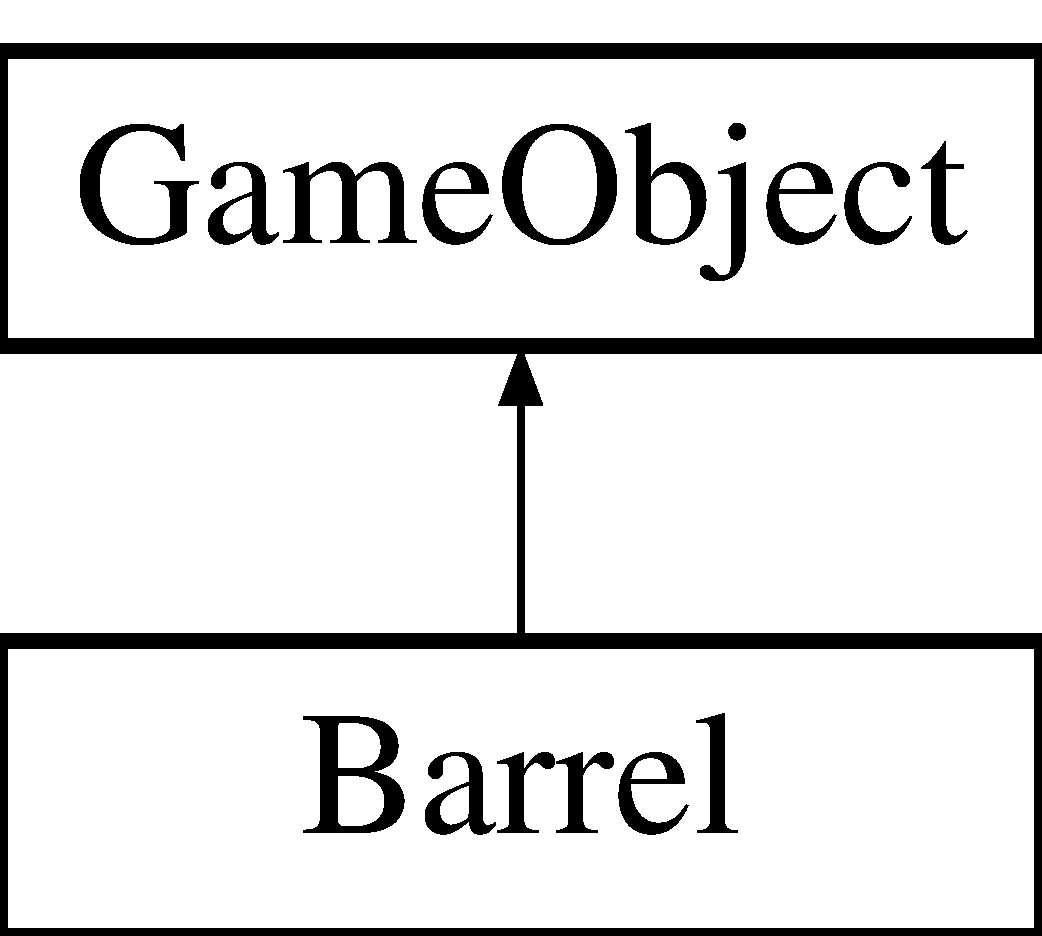
\includegraphics[height=2.000000cm]{classBarrel}
\end{center}
\end{figure}
\subsection*{Public Member Functions}
\begin{DoxyCompactItemize}
\item 
\hyperlink{classBarrel_a05e3566dcce94d44261ba799cea1966c}{Barrel} (double \hyperlink{classGameObject_a77ae10ff022a6cfe7419d4acdcffe2a4}{x}, double \hyperlink{classGameObject_af3f4a42c92fa6f6ac04d57bf4b11d43f}{y})
\item 
void \hyperlink{classBarrel_a8bfe8eeb51338bca08e3a18cb2e21460}{update} ()
\end{DoxyCompactItemize}
\subsection*{Additional Inherited Members}


\subsection{Constructor \& Destructor Documentation}
\hypertarget{classBarrel_a05e3566dcce94d44261ba799cea1966c}{\index{Barrel@{Barrel}!Barrel@{Barrel}}
\index{Barrel@{Barrel}!Barrel@{Barrel}}
\subsubsection[{Barrel}]{\setlength{\rightskip}{0pt plus 5cm}Barrel\-::\-Barrel (
\begin{DoxyParamCaption}
\item[{double}]{x, }
\item[{double}]{y}
\end{DoxyParamCaption}
)}}\label{classBarrel_a05e3566dcce94d44261ba799cea1966c}


\subsection{Member Function Documentation}
\hypertarget{classBarrel_a8bfe8eeb51338bca08e3a18cb2e21460}{\index{Barrel@{Barrel}!update@{update}}
\index{update@{update}!Barrel@{Barrel}}
\subsubsection[{update}]{\setlength{\rightskip}{0pt plus 5cm}void Barrel\-::update (
\begin{DoxyParamCaption}
{}
\end{DoxyParamCaption}
)\hspace{0.3cm}{\ttfamily [virtual]}}}\label{classBarrel_a8bfe8eeb51338bca08e3a18cb2e21460}


Implements \hyperlink{classGameObject_ae83128d0e0efef691417779605ee037c}{Game\-Object}.



The documentation for this class was generated from the following files\-:\begin{DoxyCompactItemize}
\item 
Classes/\hyperlink{Barrel_8h}{Barrel.\-h}\item 
Classes/\hyperlink{Barrel_8cpp}{Barrel.\-cpp}\end{DoxyCompactItemize}

\hypertarget{classCamera}{\section{Camera Class Reference}
\label{classCamera}\index{Camera@{Camera}}
}


{\ttfamily \#include $<$Camera.\-h$>$}

\subsection*{Public Member Functions}
\begin{DoxyCompactItemize}
\item 
\hyperlink{classCamera_ac907efd0aa3a7ff3d923299d3e8898fb}{Camera} (double \-\_\-x, double \-\_\-y, double \-\_\-dx, double \-\_\-dy)
\item 
void \hyperlink{classCamera_a1caf4aca0168afce3b3a59fd95988402}{render} (const std\-::vector$<$ std\-::vector$<$ int $>$$>$ \&world\-Map, std\-::vector$<$ \hyperlink{classGameObject}{Game\-Object} $\ast$ $>$ sprites)
\item 
void \hyperlink{classCamera_ad6694e787b4726baa6d02514e1942b31}{draw\-Mini\-Map} (const std\-::vector$<$ std\-::vector$<$ int $>$$>$ \&world\-Map)
\item 
void \hyperlink{classCamera_a815fc02ea2954af7ee50a54515a1a7a6}{clear\-Screen} ()
\item 
void \hyperlink{classCamera_abc9e8ccef4d50a39e82d7f8308416ee8}{update\-Screen} ()
\end{DoxyCompactItemize}
\subsection*{Public Attributes}
\begin{DoxyCompactItemize}
\item 
double \hyperlink{classCamera_abe152acfd445ee3ab8ab54bc4053a4b3}{p\-X}
\item 
double \hyperlink{classCamera_ab6307d4358b77bf4200c6eb6643fed75}{p\-Y}
\item 
double \hyperlink{classCamera_a3d9d9b2077ddfcd90eb887f0fa472986}{d\-X}
\item 
double \hyperlink{classCamera_a21a394585a8f656fbe39c06575afa62e}{d\-Y}
\item 
double \hyperlink{classCamera_a724db0b967f04e90c0c17c8fd9301d43}{pl\-X}
\item 
double \hyperlink{classCamera_a34e29ef2ecb4a278a91aec6db4e9f412}{pl\-Y}
\end{DoxyCompactItemize}


\subsection{Constructor \& Destructor Documentation}
\hypertarget{classCamera_ac907efd0aa3a7ff3d923299d3e8898fb}{\index{Camera@{Camera}!Camera@{Camera}}
\index{Camera@{Camera}!Camera@{Camera}}
\subsubsection[{Camera}]{\setlength{\rightskip}{0pt plus 5cm}Camera\-::\-Camera (
\begin{DoxyParamCaption}
\item[{double}]{\-\_\-x, }
\item[{double}]{\-\_\-y, }
\item[{double}]{\-\_\-dx, }
\item[{double}]{\-\_\-dy}
\end{DoxyParamCaption}
)}}\label{classCamera_ac907efd0aa3a7ff3d923299d3e8898fb}


\subsection{Member Function Documentation}
\hypertarget{classCamera_a815fc02ea2954af7ee50a54515a1a7a6}{\index{Camera@{Camera}!clear\-Screen@{clear\-Screen}}
\index{clear\-Screen@{clear\-Screen}!Camera@{Camera}}
\subsubsection[{clear\-Screen}]{\setlength{\rightskip}{0pt plus 5cm}void Camera\-::clear\-Screen (
\begin{DoxyParamCaption}
{}
\end{DoxyParamCaption}
)}}\label{classCamera_a815fc02ea2954af7ee50a54515a1a7a6}
\hypertarget{classCamera_ad6694e787b4726baa6d02514e1942b31}{\index{Camera@{Camera}!draw\-Mini\-Map@{draw\-Mini\-Map}}
\index{draw\-Mini\-Map@{draw\-Mini\-Map}!Camera@{Camera}}
\subsubsection[{draw\-Mini\-Map}]{\setlength{\rightskip}{0pt plus 5cm}void Camera\-::draw\-Mini\-Map (
\begin{DoxyParamCaption}
\item[{const std\-::vector$<$ std\-::vector$<$ int $>$$>$ \&}]{world\-Map}
\end{DoxyParamCaption}
)}}\label{classCamera_ad6694e787b4726baa6d02514e1942b31}
\hypertarget{classCamera_a1caf4aca0168afce3b3a59fd95988402}{\index{Camera@{Camera}!render@{render}}
\index{render@{render}!Camera@{Camera}}
\subsubsection[{render}]{\setlength{\rightskip}{0pt plus 5cm}void Camera\-::render (
\begin{DoxyParamCaption}
\item[{const std\-::vector$<$ std\-::vector$<$ int $>$$>$ \&}]{world\-Map, }
\item[{std\-::vector$<$ {\bf Game\-Object} $\ast$ $>$}]{sprites}
\end{DoxyParamCaption}
)}}\label{classCamera_a1caf4aca0168afce3b3a59fd95988402}
\hypertarget{classCamera_abc9e8ccef4d50a39e82d7f8308416ee8}{\index{Camera@{Camera}!update\-Screen@{update\-Screen}}
\index{update\-Screen@{update\-Screen}!Camera@{Camera}}
\subsubsection[{update\-Screen}]{\setlength{\rightskip}{0pt plus 5cm}void Camera\-::update\-Screen (
\begin{DoxyParamCaption}
{}
\end{DoxyParamCaption}
)}}\label{classCamera_abc9e8ccef4d50a39e82d7f8308416ee8}


\subsection{Member Data Documentation}
\hypertarget{classCamera_a3d9d9b2077ddfcd90eb887f0fa472986}{\index{Camera@{Camera}!d\-X@{d\-X}}
\index{d\-X@{d\-X}!Camera@{Camera}}
\subsubsection[{d\-X}]{\setlength{\rightskip}{0pt plus 5cm}double Camera\-::d\-X}}\label{classCamera_a3d9d9b2077ddfcd90eb887f0fa472986}
\hypertarget{classCamera_a21a394585a8f656fbe39c06575afa62e}{\index{Camera@{Camera}!d\-Y@{d\-Y}}
\index{d\-Y@{d\-Y}!Camera@{Camera}}
\subsubsection[{d\-Y}]{\setlength{\rightskip}{0pt plus 5cm}double Camera\-::d\-Y}}\label{classCamera_a21a394585a8f656fbe39c06575afa62e}
\hypertarget{classCamera_a724db0b967f04e90c0c17c8fd9301d43}{\index{Camera@{Camera}!pl\-X@{pl\-X}}
\index{pl\-X@{pl\-X}!Camera@{Camera}}
\subsubsection[{pl\-X}]{\setlength{\rightskip}{0pt plus 5cm}double Camera\-::pl\-X}}\label{classCamera_a724db0b967f04e90c0c17c8fd9301d43}
\hypertarget{classCamera_a34e29ef2ecb4a278a91aec6db4e9f412}{\index{Camera@{Camera}!pl\-Y@{pl\-Y}}
\index{pl\-Y@{pl\-Y}!Camera@{Camera}}
\subsubsection[{pl\-Y}]{\setlength{\rightskip}{0pt plus 5cm}double Camera\-::pl\-Y}}\label{classCamera_a34e29ef2ecb4a278a91aec6db4e9f412}
\hypertarget{classCamera_abe152acfd445ee3ab8ab54bc4053a4b3}{\index{Camera@{Camera}!p\-X@{p\-X}}
\index{p\-X@{p\-X}!Camera@{Camera}}
\subsubsection[{p\-X}]{\setlength{\rightskip}{0pt plus 5cm}double Camera\-::p\-X}}\label{classCamera_abe152acfd445ee3ab8ab54bc4053a4b3}
\hypertarget{classCamera_ab6307d4358b77bf4200c6eb6643fed75}{\index{Camera@{Camera}!p\-Y@{p\-Y}}
\index{p\-Y@{p\-Y}!Camera@{Camera}}
\subsubsection[{p\-Y}]{\setlength{\rightskip}{0pt plus 5cm}double Camera\-::p\-Y}}\label{classCamera_ab6307d4358b77bf4200c6eb6643fed75}


The documentation for this class was generated from the following files\-:\begin{DoxyCompactItemize}
\item 
Utils/\hyperlink{Camera_8h}{Camera.\-h}\item 
Utils/\hyperlink{Camera_8cpp}{Camera.\-cpp}\end{DoxyCompactItemize}

\hypertarget{structQuickCG_1_1ColorHSL}{\section{Quick\-C\-G\-:\-:Color\-H\-S\-L Struct Reference}
\label{structQuickCG_1_1ColorHSL}\index{Quick\-C\-G\-::\-Color\-H\-S\-L@{Quick\-C\-G\-::\-Color\-H\-S\-L}}
}


{\ttfamily \#include $<$quickcg.\-h$>$}

\subsection*{Public Member Functions}
\begin{DoxyCompactItemize}
\item 
\hyperlink{structQuickCG_1_1ColorHSL_af38324de505ec8bb6b0db73c8e87179c}{Color\-H\-S\-L} (Uint8 \hyperlink{structQuickCG_1_1ColorHSL_a22460cd9b83f6cfc658dfd4c6acb9dc1}{h}, Uint8 \hyperlink{structQuickCG_1_1ColorHSL_abf20406550a927b4afe96ddec60de577}{s}, Uint8 \hyperlink{structQuickCG_1_1ColorHSL_ab67c594a335b19305eee199fb64a5d61}{l})
\item 
\hyperlink{structQuickCG_1_1ColorHSL_a1517aa2b85f37af7e38429340cb9ef43}{Color\-H\-S\-L} ()
\end{DoxyCompactItemize}
\subsection*{Public Attributes}
\begin{DoxyCompactItemize}
\item 
int \hyperlink{structQuickCG_1_1ColorHSL_a22460cd9b83f6cfc658dfd4c6acb9dc1}{h}
\item 
int \hyperlink{structQuickCG_1_1ColorHSL_abf20406550a927b4afe96ddec60de577}{s}
\item 
int \hyperlink{structQuickCG_1_1ColorHSL_ab67c594a335b19305eee199fb64a5d61}{l}
\end{DoxyCompactItemize}


\subsection{Constructor \& Destructor Documentation}
\hypertarget{structQuickCG_1_1ColorHSL_af38324de505ec8bb6b0db73c8e87179c}{\index{Quick\-C\-G\-::\-Color\-H\-S\-L@{Quick\-C\-G\-::\-Color\-H\-S\-L}!Color\-H\-S\-L@{Color\-H\-S\-L}}
\index{Color\-H\-S\-L@{Color\-H\-S\-L}!QuickCG::ColorHSL@{Quick\-C\-G\-::\-Color\-H\-S\-L}}
\subsubsection[{Color\-H\-S\-L}]{\setlength{\rightskip}{0pt plus 5cm}Quick\-C\-G\-::\-Color\-H\-S\-L\-::\-Color\-H\-S\-L (
\begin{DoxyParamCaption}
\item[{Uint8}]{h, }
\item[{Uint8}]{s, }
\item[{Uint8}]{l}
\end{DoxyParamCaption}
)}}\label{structQuickCG_1_1ColorHSL_af38324de505ec8bb6b0db73c8e87179c}
\hypertarget{structQuickCG_1_1ColorHSL_a1517aa2b85f37af7e38429340cb9ef43}{\index{Quick\-C\-G\-::\-Color\-H\-S\-L@{Quick\-C\-G\-::\-Color\-H\-S\-L}!Color\-H\-S\-L@{Color\-H\-S\-L}}
\index{Color\-H\-S\-L@{Color\-H\-S\-L}!QuickCG::ColorHSL@{Quick\-C\-G\-::\-Color\-H\-S\-L}}
\subsubsection[{Color\-H\-S\-L}]{\setlength{\rightskip}{0pt plus 5cm}Quick\-C\-G\-::\-Color\-H\-S\-L\-::\-Color\-H\-S\-L (
\begin{DoxyParamCaption}
{}
\end{DoxyParamCaption}
)}}\label{structQuickCG_1_1ColorHSL_a1517aa2b85f37af7e38429340cb9ef43}


\subsection{Member Data Documentation}
\hypertarget{structQuickCG_1_1ColorHSL_a22460cd9b83f6cfc658dfd4c6acb9dc1}{\index{Quick\-C\-G\-::\-Color\-H\-S\-L@{Quick\-C\-G\-::\-Color\-H\-S\-L}!h@{h}}
\index{h@{h}!QuickCG::ColorHSL@{Quick\-C\-G\-::\-Color\-H\-S\-L}}
\subsubsection[{h}]{\setlength{\rightskip}{0pt plus 5cm}int Quick\-C\-G\-::\-Color\-H\-S\-L\-::h}}\label{structQuickCG_1_1ColorHSL_a22460cd9b83f6cfc658dfd4c6acb9dc1}
\hypertarget{structQuickCG_1_1ColorHSL_ab67c594a335b19305eee199fb64a5d61}{\index{Quick\-C\-G\-::\-Color\-H\-S\-L@{Quick\-C\-G\-::\-Color\-H\-S\-L}!l@{l}}
\index{l@{l}!QuickCG::ColorHSL@{Quick\-C\-G\-::\-Color\-H\-S\-L}}
\subsubsection[{l}]{\setlength{\rightskip}{0pt plus 5cm}int Quick\-C\-G\-::\-Color\-H\-S\-L\-::l}}\label{structQuickCG_1_1ColorHSL_ab67c594a335b19305eee199fb64a5d61}
\hypertarget{structQuickCG_1_1ColorHSL_abf20406550a927b4afe96ddec60de577}{\index{Quick\-C\-G\-::\-Color\-H\-S\-L@{Quick\-C\-G\-::\-Color\-H\-S\-L}!s@{s}}
\index{s@{s}!QuickCG::ColorHSL@{Quick\-C\-G\-::\-Color\-H\-S\-L}}
\subsubsection[{s}]{\setlength{\rightskip}{0pt plus 5cm}int Quick\-C\-G\-::\-Color\-H\-S\-L\-::s}}\label{structQuickCG_1_1ColorHSL_abf20406550a927b4afe96ddec60de577}


The documentation for this struct was generated from the following files\-:\begin{DoxyCompactItemize}
\item 
Utils/\hyperlink{quickcg_8h}{quickcg.\-h}\item 
Utils/\hyperlink{quickcg_8cpp}{quickcg.\-cpp}\end{DoxyCompactItemize}

\hypertarget{structQuickCG_1_1ColorHSV}{\section{Quick\-C\-G\-:\-:Color\-H\-S\-V Struct Reference}
\label{structQuickCG_1_1ColorHSV}\index{Quick\-C\-G\-::\-Color\-H\-S\-V@{Quick\-C\-G\-::\-Color\-H\-S\-V}}
}


{\ttfamily \#include $<$quickcg.\-h$>$}

\subsection*{Public Member Functions}
\begin{DoxyCompactItemize}
\item 
\hyperlink{structQuickCG_1_1ColorHSV_a0b545ef3534166ba240de07f83722ea8}{Color\-H\-S\-V} (Uint8 \hyperlink{structQuickCG_1_1ColorHSV_acbf27d11c4aab9e11e140c0b2e3cab72}{h}, Uint8 \hyperlink{structQuickCG_1_1ColorHSV_a458b4a97b9351221f01245e11460d4db}{s}, Uint8 \hyperlink{structQuickCG_1_1ColorHSV_ab7c052e520eb5bdaa196568da3f015a1}{v})
\item 
\hyperlink{structQuickCG_1_1ColorHSV_aa8d81269f4bc7261260c0e56c94c3ab2}{Color\-H\-S\-V} ()
\end{DoxyCompactItemize}
\subsection*{Public Attributes}
\begin{DoxyCompactItemize}
\item 
int \hyperlink{structQuickCG_1_1ColorHSV_acbf27d11c4aab9e11e140c0b2e3cab72}{h}
\item 
int \hyperlink{structQuickCG_1_1ColorHSV_a458b4a97b9351221f01245e11460d4db}{s}
\item 
int \hyperlink{structQuickCG_1_1ColorHSV_ab7c052e520eb5bdaa196568da3f015a1}{v}
\end{DoxyCompactItemize}


\subsection{Constructor \& Destructor Documentation}
\hypertarget{structQuickCG_1_1ColorHSV_a0b545ef3534166ba240de07f83722ea8}{\index{Quick\-C\-G\-::\-Color\-H\-S\-V@{Quick\-C\-G\-::\-Color\-H\-S\-V}!Color\-H\-S\-V@{Color\-H\-S\-V}}
\index{Color\-H\-S\-V@{Color\-H\-S\-V}!QuickCG::ColorHSV@{Quick\-C\-G\-::\-Color\-H\-S\-V}}
\subsubsection[{Color\-H\-S\-V}]{\setlength{\rightskip}{0pt plus 5cm}Quick\-C\-G\-::\-Color\-H\-S\-V\-::\-Color\-H\-S\-V (
\begin{DoxyParamCaption}
\item[{Uint8}]{h, }
\item[{Uint8}]{s, }
\item[{Uint8}]{v}
\end{DoxyParamCaption}
)}}\label{structQuickCG_1_1ColorHSV_a0b545ef3534166ba240de07f83722ea8}
\hypertarget{structQuickCG_1_1ColorHSV_aa8d81269f4bc7261260c0e56c94c3ab2}{\index{Quick\-C\-G\-::\-Color\-H\-S\-V@{Quick\-C\-G\-::\-Color\-H\-S\-V}!Color\-H\-S\-V@{Color\-H\-S\-V}}
\index{Color\-H\-S\-V@{Color\-H\-S\-V}!QuickCG::ColorHSV@{Quick\-C\-G\-::\-Color\-H\-S\-V}}
\subsubsection[{Color\-H\-S\-V}]{\setlength{\rightskip}{0pt plus 5cm}Quick\-C\-G\-::\-Color\-H\-S\-V\-::\-Color\-H\-S\-V (
\begin{DoxyParamCaption}
{}
\end{DoxyParamCaption}
)}}\label{structQuickCG_1_1ColorHSV_aa8d81269f4bc7261260c0e56c94c3ab2}


\subsection{Member Data Documentation}
\hypertarget{structQuickCG_1_1ColorHSV_acbf27d11c4aab9e11e140c0b2e3cab72}{\index{Quick\-C\-G\-::\-Color\-H\-S\-V@{Quick\-C\-G\-::\-Color\-H\-S\-V}!h@{h}}
\index{h@{h}!QuickCG::ColorHSV@{Quick\-C\-G\-::\-Color\-H\-S\-V}}
\subsubsection[{h}]{\setlength{\rightskip}{0pt plus 5cm}int Quick\-C\-G\-::\-Color\-H\-S\-V\-::h}}\label{structQuickCG_1_1ColorHSV_acbf27d11c4aab9e11e140c0b2e3cab72}
\hypertarget{structQuickCG_1_1ColorHSV_a458b4a97b9351221f01245e11460d4db}{\index{Quick\-C\-G\-::\-Color\-H\-S\-V@{Quick\-C\-G\-::\-Color\-H\-S\-V}!s@{s}}
\index{s@{s}!QuickCG::ColorHSV@{Quick\-C\-G\-::\-Color\-H\-S\-V}}
\subsubsection[{s}]{\setlength{\rightskip}{0pt plus 5cm}int Quick\-C\-G\-::\-Color\-H\-S\-V\-::s}}\label{structQuickCG_1_1ColorHSV_a458b4a97b9351221f01245e11460d4db}
\hypertarget{structQuickCG_1_1ColorHSV_ab7c052e520eb5bdaa196568da3f015a1}{\index{Quick\-C\-G\-::\-Color\-H\-S\-V@{Quick\-C\-G\-::\-Color\-H\-S\-V}!v@{v}}
\index{v@{v}!QuickCG::ColorHSV@{Quick\-C\-G\-::\-Color\-H\-S\-V}}
\subsubsection[{v}]{\setlength{\rightskip}{0pt plus 5cm}int Quick\-C\-G\-::\-Color\-H\-S\-V\-::v}}\label{structQuickCG_1_1ColorHSV_ab7c052e520eb5bdaa196568da3f015a1}


The documentation for this struct was generated from the following files\-:\begin{DoxyCompactItemize}
\item 
Utils/\hyperlink{quickcg_8h}{quickcg.\-h}\item 
Utils/\hyperlink{quickcg_8cpp}{quickcg.\-cpp}\end{DoxyCompactItemize}

\hypertarget{structQuickCG_1_1ColorRGB}{\section{Quick\-C\-G\-:\-:Color\-R\-G\-B Struct Reference}
\label{structQuickCG_1_1ColorRGB}\index{Quick\-C\-G\-::\-Color\-R\-G\-B@{Quick\-C\-G\-::\-Color\-R\-G\-B}}
}


{\ttfamily \#include $<$quickcg.\-h$>$}

\subsection*{Public Member Functions}
\begin{DoxyCompactItemize}
\item 
\hyperlink{structQuickCG_1_1ColorRGB_a4f9b2654955a752589ba46f02ce64d57}{Color\-R\-G\-B} (Uint8 \hyperlink{structQuickCG_1_1ColorRGB_a3873210b09a441c02ec224cfc49b8385}{r}, Uint8 \hyperlink{structQuickCG_1_1ColorRGB_af9d258f0404f8dc39677ccc6a474e36a}{g}, Uint8 \hyperlink{structQuickCG_1_1ColorRGB_ae85c3461b4eaed0bf2ccdf07f4bbedb4}{b})
\item 
\hyperlink{structQuickCG_1_1ColorRGB_a35046c5329affabfae8d491fda700916}{Color\-R\-G\-B} (const \hyperlink{structQuickCG_1_1ColorRGB8bit}{Color\-R\-G\-B8bit} \&color)
\item 
\hyperlink{structQuickCG_1_1ColorRGB_a5b4b7e30ad5f4daf9189354751058986}{Color\-R\-G\-B} ()
\end{DoxyCompactItemize}
\subsection*{Public Attributes}
\begin{DoxyCompactItemize}
\item 
int \hyperlink{structQuickCG_1_1ColorRGB_a3873210b09a441c02ec224cfc49b8385}{r}
\item 
int \hyperlink{structQuickCG_1_1ColorRGB_af9d258f0404f8dc39677ccc6a474e36a}{g}
\item 
int \hyperlink{structQuickCG_1_1ColorRGB_ae85c3461b4eaed0bf2ccdf07f4bbedb4}{b}
\end{DoxyCompactItemize}


\subsection{Constructor \& Destructor Documentation}
\hypertarget{structQuickCG_1_1ColorRGB_a4f9b2654955a752589ba46f02ce64d57}{\index{Quick\-C\-G\-::\-Color\-R\-G\-B@{Quick\-C\-G\-::\-Color\-R\-G\-B}!Color\-R\-G\-B@{Color\-R\-G\-B}}
\index{Color\-R\-G\-B@{Color\-R\-G\-B}!QuickCG::ColorRGB@{Quick\-C\-G\-::\-Color\-R\-G\-B}}
\subsubsection[{Color\-R\-G\-B}]{\setlength{\rightskip}{0pt plus 5cm}Quick\-C\-G\-::\-Color\-R\-G\-B\-::\-Color\-R\-G\-B (
\begin{DoxyParamCaption}
\item[{Uint8}]{r, }
\item[{Uint8}]{g, }
\item[{Uint8}]{b}
\end{DoxyParamCaption}
)}}\label{structQuickCG_1_1ColorRGB_a4f9b2654955a752589ba46f02ce64d57}
\hypertarget{structQuickCG_1_1ColorRGB_a35046c5329affabfae8d491fda700916}{\index{Quick\-C\-G\-::\-Color\-R\-G\-B@{Quick\-C\-G\-::\-Color\-R\-G\-B}!Color\-R\-G\-B@{Color\-R\-G\-B}}
\index{Color\-R\-G\-B@{Color\-R\-G\-B}!QuickCG::ColorRGB@{Quick\-C\-G\-::\-Color\-R\-G\-B}}
\subsubsection[{Color\-R\-G\-B}]{\setlength{\rightskip}{0pt plus 5cm}Quick\-C\-G\-::\-Color\-R\-G\-B\-::\-Color\-R\-G\-B (
\begin{DoxyParamCaption}
\item[{const {\bf Color\-R\-G\-B8bit} \&}]{color}
\end{DoxyParamCaption}
)}}\label{structQuickCG_1_1ColorRGB_a35046c5329affabfae8d491fda700916}
\hypertarget{structQuickCG_1_1ColorRGB_a5b4b7e30ad5f4daf9189354751058986}{\index{Quick\-C\-G\-::\-Color\-R\-G\-B@{Quick\-C\-G\-::\-Color\-R\-G\-B}!Color\-R\-G\-B@{Color\-R\-G\-B}}
\index{Color\-R\-G\-B@{Color\-R\-G\-B}!QuickCG::ColorRGB@{Quick\-C\-G\-::\-Color\-R\-G\-B}}
\subsubsection[{Color\-R\-G\-B}]{\setlength{\rightskip}{0pt plus 5cm}Quick\-C\-G\-::\-Color\-R\-G\-B\-::\-Color\-R\-G\-B (
\begin{DoxyParamCaption}
{}
\end{DoxyParamCaption}
)}}\label{structQuickCG_1_1ColorRGB_a5b4b7e30ad5f4daf9189354751058986}


\subsection{Member Data Documentation}
\hypertarget{structQuickCG_1_1ColorRGB_ae85c3461b4eaed0bf2ccdf07f4bbedb4}{\index{Quick\-C\-G\-::\-Color\-R\-G\-B@{Quick\-C\-G\-::\-Color\-R\-G\-B}!b@{b}}
\index{b@{b}!QuickCG::ColorRGB@{Quick\-C\-G\-::\-Color\-R\-G\-B}}
\subsubsection[{b}]{\setlength{\rightskip}{0pt plus 5cm}int Quick\-C\-G\-::\-Color\-R\-G\-B\-::b}}\label{structQuickCG_1_1ColorRGB_ae85c3461b4eaed0bf2ccdf07f4bbedb4}
\hypertarget{structQuickCG_1_1ColorRGB_af9d258f0404f8dc39677ccc6a474e36a}{\index{Quick\-C\-G\-::\-Color\-R\-G\-B@{Quick\-C\-G\-::\-Color\-R\-G\-B}!g@{g}}
\index{g@{g}!QuickCG::ColorRGB@{Quick\-C\-G\-::\-Color\-R\-G\-B}}
\subsubsection[{g}]{\setlength{\rightskip}{0pt plus 5cm}int Quick\-C\-G\-::\-Color\-R\-G\-B\-::g}}\label{structQuickCG_1_1ColorRGB_af9d258f0404f8dc39677ccc6a474e36a}
\hypertarget{structQuickCG_1_1ColorRGB_a3873210b09a441c02ec224cfc49b8385}{\index{Quick\-C\-G\-::\-Color\-R\-G\-B@{Quick\-C\-G\-::\-Color\-R\-G\-B}!r@{r}}
\index{r@{r}!QuickCG::ColorRGB@{Quick\-C\-G\-::\-Color\-R\-G\-B}}
\subsubsection[{r}]{\setlength{\rightskip}{0pt plus 5cm}int Quick\-C\-G\-::\-Color\-R\-G\-B\-::r}}\label{structQuickCG_1_1ColorRGB_a3873210b09a441c02ec224cfc49b8385}


The documentation for this struct was generated from the following files\-:\begin{DoxyCompactItemize}
\item 
Utils/\hyperlink{quickcg_8h}{quickcg.\-h}\item 
Utils/\hyperlink{quickcg_8cpp}{quickcg.\-cpp}\end{DoxyCompactItemize}

\hypertarget{structQuickCG_1_1ColorRGB8bit}{\section{Quick\-C\-G\-:\-:Color\-R\-G\-B8bit Struct Reference}
\label{structQuickCG_1_1ColorRGB8bit}\index{Quick\-C\-G\-::\-Color\-R\-G\-B8bit@{Quick\-C\-G\-::\-Color\-R\-G\-B8bit}}
}


{\ttfamily \#include $<$quickcg.\-h$>$}

\subsection*{Public Member Functions}
\begin{DoxyCompactItemize}
\item 
\hyperlink{structQuickCG_1_1ColorRGB8bit_a6aad15726fbe6fabf1b2ffa477bc3202}{Color\-R\-G\-B8bit} (Uint8 \hyperlink{structQuickCG_1_1ColorRGB8bit_adbcc046ebfa38ac05446b51f341363f9}{r}, Uint8 \hyperlink{structQuickCG_1_1ColorRGB8bit_a04249198bd045324503af50b82ddf923}{g}, Uint8 \hyperlink{structQuickCG_1_1ColorRGB8bit_a6f74056a1bc52437a5e9c4c0af4177b7}{b})
\item 
\hyperlink{structQuickCG_1_1ColorRGB8bit_a2ad9498e869fb61d884b482baf247087}{Color\-R\-G\-B8bit} (const \hyperlink{structQuickCG_1_1ColorRGB}{Color\-R\-G\-B} \&color)
\item 
\hyperlink{structQuickCG_1_1ColorRGB8bit_a53d8d2b7e6935909928c18a62554f087}{Color\-R\-G\-B8bit} ()
\end{DoxyCompactItemize}
\subsection*{Public Attributes}
\begin{DoxyCompactItemize}
\item 
Uint8 \hyperlink{structQuickCG_1_1ColorRGB8bit_adbcc046ebfa38ac05446b51f341363f9}{r}
\item 
Uint8 \hyperlink{structQuickCG_1_1ColorRGB8bit_a04249198bd045324503af50b82ddf923}{g}
\item 
Uint8 \hyperlink{structQuickCG_1_1ColorRGB8bit_a6f74056a1bc52437a5e9c4c0af4177b7}{b}
\end{DoxyCompactItemize}


\subsection{Constructor \& Destructor Documentation}
\hypertarget{structQuickCG_1_1ColorRGB8bit_a6aad15726fbe6fabf1b2ffa477bc3202}{\index{Quick\-C\-G\-::\-Color\-R\-G\-B8bit@{Quick\-C\-G\-::\-Color\-R\-G\-B8bit}!Color\-R\-G\-B8bit@{Color\-R\-G\-B8bit}}
\index{Color\-R\-G\-B8bit@{Color\-R\-G\-B8bit}!QuickCG::ColorRGB8bit@{Quick\-C\-G\-::\-Color\-R\-G\-B8bit}}
\subsubsection[{Color\-R\-G\-B8bit}]{\setlength{\rightskip}{0pt plus 5cm}Quick\-C\-G\-::\-Color\-R\-G\-B8bit\-::\-Color\-R\-G\-B8bit (
\begin{DoxyParamCaption}
\item[{Uint8}]{r, }
\item[{Uint8}]{g, }
\item[{Uint8}]{b}
\end{DoxyParamCaption}
)}}\label{structQuickCG_1_1ColorRGB8bit_a6aad15726fbe6fabf1b2ffa477bc3202}
\hypertarget{structQuickCG_1_1ColorRGB8bit_a2ad9498e869fb61d884b482baf247087}{\index{Quick\-C\-G\-::\-Color\-R\-G\-B8bit@{Quick\-C\-G\-::\-Color\-R\-G\-B8bit}!Color\-R\-G\-B8bit@{Color\-R\-G\-B8bit}}
\index{Color\-R\-G\-B8bit@{Color\-R\-G\-B8bit}!QuickCG::ColorRGB8bit@{Quick\-C\-G\-::\-Color\-R\-G\-B8bit}}
\subsubsection[{Color\-R\-G\-B8bit}]{\setlength{\rightskip}{0pt plus 5cm}Quick\-C\-G\-::\-Color\-R\-G\-B8bit\-::\-Color\-R\-G\-B8bit (
\begin{DoxyParamCaption}
\item[{const {\bf Color\-R\-G\-B} \&}]{color}
\end{DoxyParamCaption}
)}}\label{structQuickCG_1_1ColorRGB8bit_a2ad9498e869fb61d884b482baf247087}
\hypertarget{structQuickCG_1_1ColorRGB8bit_a53d8d2b7e6935909928c18a62554f087}{\index{Quick\-C\-G\-::\-Color\-R\-G\-B8bit@{Quick\-C\-G\-::\-Color\-R\-G\-B8bit}!Color\-R\-G\-B8bit@{Color\-R\-G\-B8bit}}
\index{Color\-R\-G\-B8bit@{Color\-R\-G\-B8bit}!QuickCG::ColorRGB8bit@{Quick\-C\-G\-::\-Color\-R\-G\-B8bit}}
\subsubsection[{Color\-R\-G\-B8bit}]{\setlength{\rightskip}{0pt plus 5cm}Quick\-C\-G\-::\-Color\-R\-G\-B8bit\-::\-Color\-R\-G\-B8bit (
\begin{DoxyParamCaption}
{}
\end{DoxyParamCaption}
)}}\label{structQuickCG_1_1ColorRGB8bit_a53d8d2b7e6935909928c18a62554f087}


\subsection{Member Data Documentation}
\hypertarget{structQuickCG_1_1ColorRGB8bit_a6f74056a1bc52437a5e9c4c0af4177b7}{\index{Quick\-C\-G\-::\-Color\-R\-G\-B8bit@{Quick\-C\-G\-::\-Color\-R\-G\-B8bit}!b@{b}}
\index{b@{b}!QuickCG::ColorRGB8bit@{Quick\-C\-G\-::\-Color\-R\-G\-B8bit}}
\subsubsection[{b}]{\setlength{\rightskip}{0pt plus 5cm}Uint8 Quick\-C\-G\-::\-Color\-R\-G\-B8bit\-::b}}\label{structQuickCG_1_1ColorRGB8bit_a6f74056a1bc52437a5e9c4c0af4177b7}
\hypertarget{structQuickCG_1_1ColorRGB8bit_a04249198bd045324503af50b82ddf923}{\index{Quick\-C\-G\-::\-Color\-R\-G\-B8bit@{Quick\-C\-G\-::\-Color\-R\-G\-B8bit}!g@{g}}
\index{g@{g}!QuickCG::ColorRGB8bit@{Quick\-C\-G\-::\-Color\-R\-G\-B8bit}}
\subsubsection[{g}]{\setlength{\rightskip}{0pt plus 5cm}Uint8 Quick\-C\-G\-::\-Color\-R\-G\-B8bit\-::g}}\label{structQuickCG_1_1ColorRGB8bit_a04249198bd045324503af50b82ddf923}
\hypertarget{structQuickCG_1_1ColorRGB8bit_adbcc046ebfa38ac05446b51f341363f9}{\index{Quick\-C\-G\-::\-Color\-R\-G\-B8bit@{Quick\-C\-G\-::\-Color\-R\-G\-B8bit}!r@{r}}
\index{r@{r}!QuickCG::ColorRGB8bit@{Quick\-C\-G\-::\-Color\-R\-G\-B8bit}}
\subsubsection[{r}]{\setlength{\rightskip}{0pt plus 5cm}Uint8 Quick\-C\-G\-::\-Color\-R\-G\-B8bit\-::r}}\label{structQuickCG_1_1ColorRGB8bit_adbcc046ebfa38ac05446b51f341363f9}


The documentation for this struct was generated from the following files\-:\begin{DoxyCompactItemize}
\item 
Utils/\hyperlink{quickcg_8h}{quickcg.\-h}\item 
Utils/\hyperlink{quickcg_8cpp}{quickcg.\-cpp}\end{DoxyCompactItemize}

\hypertarget{classComponent}{\section{Component Class Reference}
\label{classComponent}\index{Component@{Component}}
}


{\ttfamily \#include $<$Component.\-h$>$}



The documentation for this class was generated from the following file\-:\begin{DoxyCompactItemize}
\item 
Classes/\hyperlink{Component_8h}{Component.\-h}\end{DoxyCompactItemize}

\hypertarget{classConfigFileParser}{\section{Config\-File\-Parser Class Reference}
\label{classConfigFileParser}\index{Config\-File\-Parser@{Config\-File\-Parser}}
}


{\ttfamily \#include $<$Config\-File\-Parser.\-h$>$}

\subsection*{Public Member Functions}
\begin{DoxyCompactItemize}
\item 
\hyperlink{classConfigFileParser_ababdbb96452d3e39677e434b3439f6df}{Config\-File\-Parser} ()
\item 
Json\-::\-Value \hyperlink{classConfigFileParser_a367a634885b1877e5d50fcafcf36cc82}{load\-File} (std\-::string filename)
\item 
Json\-::\-Value \hyperlink{classConfigFileParser_a274bffad1419f68e46b0122ee39073a0}{get} (std\-::string key)
\item 
Json\-::\-Value \hyperlink{classConfigFileParser_a5ed322c51117f33eb8e871374b26f065}{get} (std\-::string key, Json\-::\-Value notfound)
\end{DoxyCompactItemize}
\subsection*{Public Attributes}
\begin{DoxyCompactItemize}
\item 
Json\-::\-Value \hyperlink{classConfigFileParser_a61cfe04569f4b8864352068cf1a60475}{root}
\end{DoxyCompactItemize}
\subsection*{Static Public Attributes}
\begin{DoxyCompactItemize}
\item 
static const Json\-::\-Value \hyperlink{classConfigFileParser_a3f5b477413c70e4364d68345ebec52a1}{V\-A\-L\-U\-E\-\_\-\-N\-O\-T\-\_\-\-F\-O\-U\-N\-D} = Json\-::\-Value\-::null
\item 
static const std\-::string \hyperlink{classConfigFileParser_a03d130795beded6ace2b5d9b2e120216}{D\-A\-T\-A\-\_\-\-F\-O\-L\-D\-E\-R} = \char`\"{}./Data/\char`\"{}
\end{DoxyCompactItemize}


\subsection{Constructor \& Destructor Documentation}
\hypertarget{classConfigFileParser_ababdbb96452d3e39677e434b3439f6df}{\index{Config\-File\-Parser@{Config\-File\-Parser}!Config\-File\-Parser@{Config\-File\-Parser}}
\index{Config\-File\-Parser@{Config\-File\-Parser}!ConfigFileParser@{Config\-File\-Parser}}
\subsubsection[{Config\-File\-Parser}]{\setlength{\rightskip}{0pt plus 5cm}Config\-File\-Parser\-::\-Config\-File\-Parser (
\begin{DoxyParamCaption}
{}
\end{DoxyParamCaption}
)}}\label{classConfigFileParser_ababdbb96452d3e39677e434b3439f6df}


\subsection{Member Function Documentation}
\hypertarget{classConfigFileParser_a274bffad1419f68e46b0122ee39073a0}{\index{Config\-File\-Parser@{Config\-File\-Parser}!get@{get}}
\index{get@{get}!ConfigFileParser@{Config\-File\-Parser}}
\subsubsection[{get}]{\setlength{\rightskip}{0pt plus 5cm}Json\-::\-Value Config\-File\-Parser\-::get (
\begin{DoxyParamCaption}
\item[{std\-::string}]{key}
\end{DoxyParamCaption}
)}}\label{classConfigFileParser_a274bffad1419f68e46b0122ee39073a0}
\hypertarget{classConfigFileParser_a5ed322c51117f33eb8e871374b26f065}{\index{Config\-File\-Parser@{Config\-File\-Parser}!get@{get}}
\index{get@{get}!ConfigFileParser@{Config\-File\-Parser}}
\subsubsection[{get}]{\setlength{\rightskip}{0pt plus 5cm}Json\-::\-Value Config\-File\-Parser\-::get (
\begin{DoxyParamCaption}
\item[{std\-::string}]{key, }
\item[{Json\-::\-Value}]{notfound}
\end{DoxyParamCaption}
)}}\label{classConfigFileParser_a5ed322c51117f33eb8e871374b26f065}
\hypertarget{classConfigFileParser_a367a634885b1877e5d50fcafcf36cc82}{\index{Config\-File\-Parser@{Config\-File\-Parser}!load\-File@{load\-File}}
\index{load\-File@{load\-File}!ConfigFileParser@{Config\-File\-Parser}}
\subsubsection[{load\-File}]{\setlength{\rightskip}{0pt plus 5cm}Json\-::\-Value Config\-File\-Parser\-::load\-File (
\begin{DoxyParamCaption}
\item[{std\-::string}]{filename}
\end{DoxyParamCaption}
)}}\label{classConfigFileParser_a367a634885b1877e5d50fcafcf36cc82}


\subsection{Member Data Documentation}
\hypertarget{classConfigFileParser_a03d130795beded6ace2b5d9b2e120216}{\index{Config\-File\-Parser@{Config\-File\-Parser}!D\-A\-T\-A\-\_\-\-F\-O\-L\-D\-E\-R@{D\-A\-T\-A\-\_\-\-F\-O\-L\-D\-E\-R}}
\index{D\-A\-T\-A\-\_\-\-F\-O\-L\-D\-E\-R@{D\-A\-T\-A\-\_\-\-F\-O\-L\-D\-E\-R}!ConfigFileParser@{Config\-File\-Parser}}
\subsubsection[{D\-A\-T\-A\-\_\-\-F\-O\-L\-D\-E\-R}]{\setlength{\rightskip}{0pt plus 5cm}const std\-::string Config\-File\-Parser\-::\-D\-A\-T\-A\-\_\-\-F\-O\-L\-D\-E\-R = \char`\"{}./Data/\char`\"{}\hspace{0.3cm}{\ttfamily [static]}}}\label{classConfigFileParser_a03d130795beded6ace2b5d9b2e120216}
\hypertarget{classConfigFileParser_a61cfe04569f4b8864352068cf1a60475}{\index{Config\-File\-Parser@{Config\-File\-Parser}!root@{root}}
\index{root@{root}!ConfigFileParser@{Config\-File\-Parser}}
\subsubsection[{root}]{\setlength{\rightskip}{0pt plus 5cm}Json\-::\-Value Config\-File\-Parser\-::root}}\label{classConfigFileParser_a61cfe04569f4b8864352068cf1a60475}
\hypertarget{classConfigFileParser_a3f5b477413c70e4364d68345ebec52a1}{\index{Config\-File\-Parser@{Config\-File\-Parser}!V\-A\-L\-U\-E\-\_\-\-N\-O\-T\-\_\-\-F\-O\-U\-N\-D@{V\-A\-L\-U\-E\-\_\-\-N\-O\-T\-\_\-\-F\-O\-U\-N\-D}}
\index{V\-A\-L\-U\-E\-\_\-\-N\-O\-T\-\_\-\-F\-O\-U\-N\-D@{V\-A\-L\-U\-E\-\_\-\-N\-O\-T\-\_\-\-F\-O\-U\-N\-D}!ConfigFileParser@{Config\-File\-Parser}}
\subsubsection[{V\-A\-L\-U\-E\-\_\-\-N\-O\-T\-\_\-\-F\-O\-U\-N\-D}]{\setlength{\rightskip}{0pt plus 5cm}const Json\-::\-Value Config\-File\-Parser\-::\-V\-A\-L\-U\-E\-\_\-\-N\-O\-T\-\_\-\-F\-O\-U\-N\-D = Json\-::\-Value\-::null\hspace{0.3cm}{\ttfamily [static]}}}\label{classConfigFileParser_a3f5b477413c70e4364d68345ebec52a1}


The documentation for this class was generated from the following files\-:\begin{DoxyCompactItemize}
\item 
Utils/\hyperlink{ConfigFileParser_8h}{Config\-File\-Parser.\-h}\item 
Utils/\hyperlink{ConfigFileParser_8cpp}{Config\-File\-Parser.\-cpp}\end{DoxyCompactItemize}

\hypertarget{classEnemy}{\section{Enemy Class Reference}
\label{classEnemy}\index{Enemy@{Enemy}}
}


{\ttfamily \#include $<$Enemy.\-h$>$}

Inheritance diagram for Enemy\-:\begin{figure}[H]
\begin{center}
\leavevmode
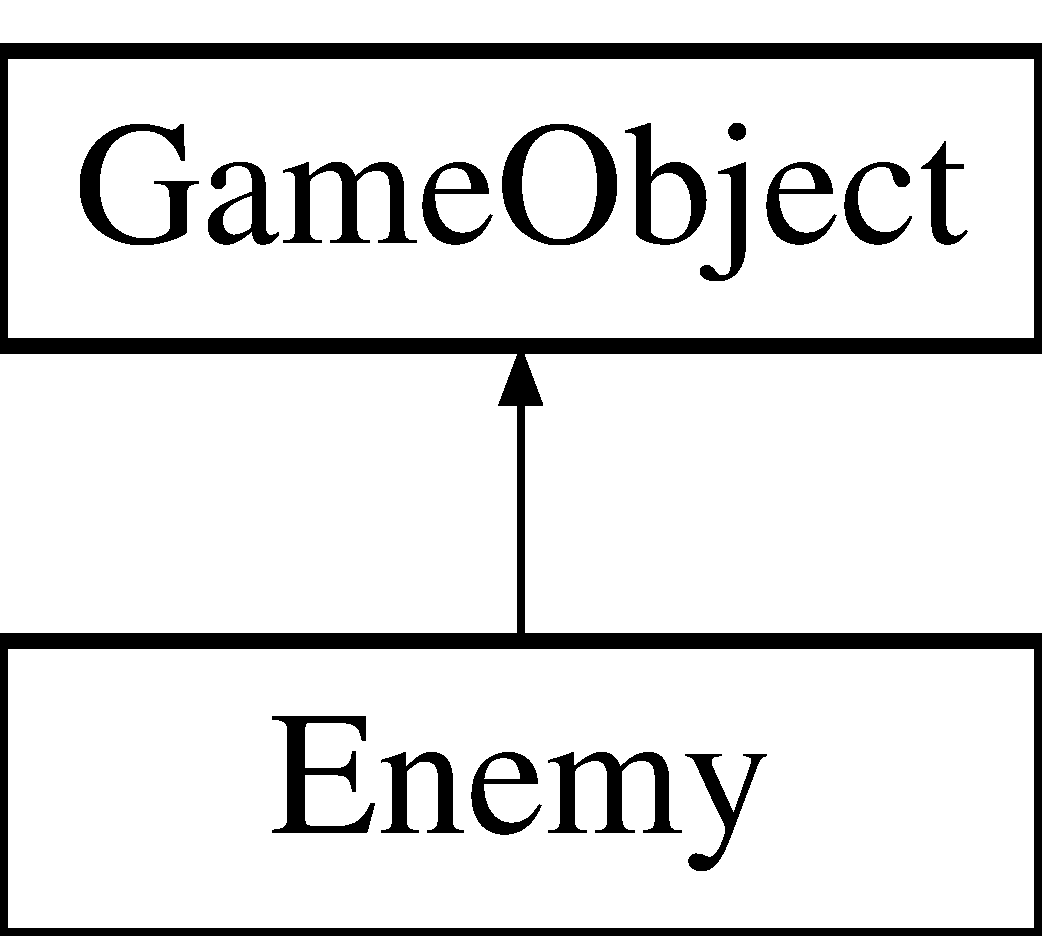
\includegraphics[height=2.000000cm]{classEnemy}
\end{center}
\end{figure}
\subsection*{Public Member Functions}
\begin{DoxyCompactItemize}
\item 
\hyperlink{classEnemy_a4d7753c9758849a2d37b4086f052d73a}{Enemy} (double \hyperlink{classGameObject_a77ae10ff022a6cfe7419d4acdcffe2a4}{x}, double \hyperlink{classGameObject_af3f4a42c92fa6f6ac04d57bf4b11d43f}{y})
\item 
void \hyperlink{classEnemy_ad55ee71b5a8c23fbd00b3c368b90cc64}{update} ()
\end{DoxyCompactItemize}
\subsection*{Additional Inherited Members}


\subsection{Constructor \& Destructor Documentation}
\hypertarget{classEnemy_a4d7753c9758849a2d37b4086f052d73a}{\index{Enemy@{Enemy}!Enemy@{Enemy}}
\index{Enemy@{Enemy}!Enemy@{Enemy}}
\subsubsection[{Enemy}]{\setlength{\rightskip}{0pt plus 5cm}Enemy\-::\-Enemy (
\begin{DoxyParamCaption}
\item[{double}]{x, }
\item[{double}]{y}
\end{DoxyParamCaption}
)}}\label{classEnemy_a4d7753c9758849a2d37b4086f052d73a}


\subsection{Member Function Documentation}
\hypertarget{classEnemy_ad55ee71b5a8c23fbd00b3c368b90cc64}{\index{Enemy@{Enemy}!update@{update}}
\index{update@{update}!Enemy@{Enemy}}
\subsubsection[{update}]{\setlength{\rightskip}{0pt plus 5cm}void Enemy\-::update (
\begin{DoxyParamCaption}
{}
\end{DoxyParamCaption}
)\hspace{0.3cm}{\ttfamily [virtual]}}}\label{classEnemy_ad55ee71b5a8c23fbd00b3c368b90cc64}


Implements \hyperlink{classGameObject_ae83128d0e0efef691417779605ee037c}{Game\-Object}.



The documentation for this class was generated from the following files\-:\begin{DoxyCompactItemize}
\item 
Classes/\hyperlink{Enemy_8h}{Enemy.\-h}\item 
Classes/\hyperlink{Enemy_8cpp}{Enemy.\-cpp}\end{DoxyCompactItemize}

\hypertarget{classGame}{\section{Game Class Reference}
\label{classGame}\index{Game@{Game}}
}


{\ttfamily \#include $<$Ruby\-Ray.\-h$>$}

\subsection*{Public Member Functions}
\begin{DoxyCompactItemize}
\item 
\hyperlink{classGame_ad59df6562a58a614fda24622d3715b65}{Game} ()
\item 
void \hyperlink{classGame_a90e2bfe9daf6de5ff1fee58a69b8fca2}{Main\-Loop} ()
\end{DoxyCompactItemize}
\subsection*{Public Attributes}
\begin{DoxyCompactItemize}
\item 
\hyperlink{classPlayer}{Player} $\ast$ \hyperlink{classGame_abec70aa1c0269a9a7e171af4d79e08bf}{player}
\item 
\hyperlink{classLevel}{Level} $\ast$ \hyperlink{classGame_a32a97a8e3bd409686e5a7a4a34b73b80}{cur\-Level}
\end{DoxyCompactItemize}


\subsection{Constructor \& Destructor Documentation}
\hypertarget{classGame_ad59df6562a58a614fda24622d3715b65}{\index{Game@{Game}!Game@{Game}}
\index{Game@{Game}!Game@{Game}}
\subsubsection[{Game}]{\setlength{\rightskip}{0pt plus 5cm}Game\-::\-Game (
\begin{DoxyParamCaption}
{}
\end{DoxyParamCaption}
)}}\label{classGame_ad59df6562a58a614fda24622d3715b65}


\subsection{Member Function Documentation}
\hypertarget{classGame_a90e2bfe9daf6de5ff1fee58a69b8fca2}{\index{Game@{Game}!Main\-Loop@{Main\-Loop}}
\index{Main\-Loop@{Main\-Loop}!Game@{Game}}
\subsubsection[{Main\-Loop}]{\setlength{\rightskip}{0pt plus 5cm}void Game\-::\-Main\-Loop (
\begin{DoxyParamCaption}
{}
\end{DoxyParamCaption}
)}}\label{classGame_a90e2bfe9daf6de5ff1fee58a69b8fca2}


\subsection{Member Data Documentation}
\hypertarget{classGame_a32a97a8e3bd409686e5a7a4a34b73b80}{\index{Game@{Game}!cur\-Level@{cur\-Level}}
\index{cur\-Level@{cur\-Level}!Game@{Game}}
\subsubsection[{cur\-Level}]{\setlength{\rightskip}{0pt plus 5cm}{\bf Level}$\ast$ Game\-::cur\-Level}}\label{classGame_a32a97a8e3bd409686e5a7a4a34b73b80}
\hypertarget{classGame_abec70aa1c0269a9a7e171af4d79e08bf}{\index{Game@{Game}!player@{player}}
\index{player@{player}!Game@{Game}}
\subsubsection[{player}]{\setlength{\rightskip}{0pt plus 5cm}{\bf Player}$\ast$ Game\-::player}}\label{classGame_abec70aa1c0269a9a7e171af4d79e08bf}


The documentation for this class was generated from the following files\-:\begin{DoxyCompactItemize}
\item 
Classes/\hyperlink{RubyRay_8h}{Ruby\-Ray.\-h}\item 
Classes/\hyperlink{RubyRay_8cpp}{Ruby\-Ray.\-cpp}\end{DoxyCompactItemize}

\hypertarget{classGameObject}{\section{Game\-Object Class Reference}
\label{classGameObject}\index{Game\-Object@{Game\-Object}}
}


This is the base class for any interactable object in the game.  




{\ttfamily \#include $<$Game\-Object.\-h$>$}

Inheritance diagram for Game\-Object\-:\begin{figure}[H]
\begin{center}
\leavevmode
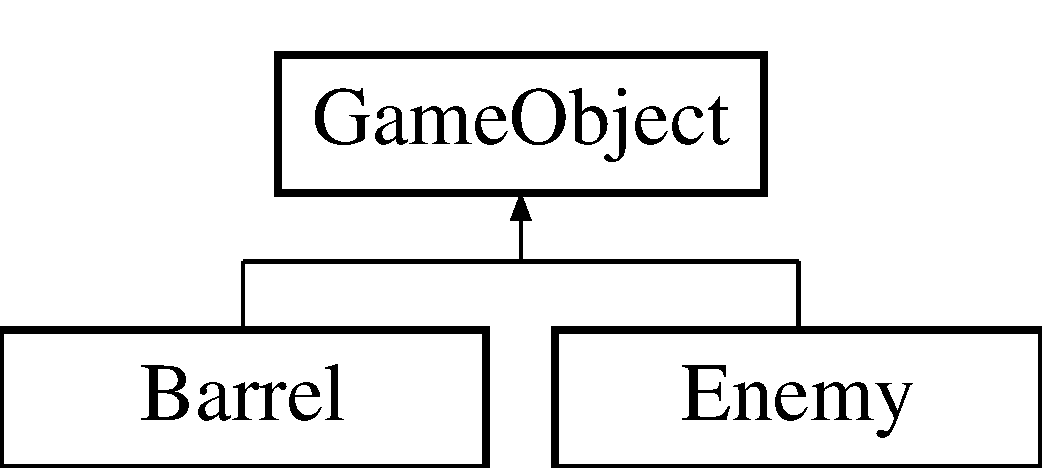
\includegraphics[height=2.000000cm]{classGameObject}
\end{center}
\end{figure}
\subsection*{Public Member Functions}
\begin{DoxyCompactItemize}
\item 
\hyperlink{classGameObject_a0348e3ee2e83d56eafca7a3547f432c4}{Game\-Object} ()
\item 
void \hyperlink{classGameObject_aec6d8e80fc3b484b5664630f2c33a19c}{add\-Component} (std\-::type\-\_\-index, \hyperlink{classComponent}{Component} $\ast$c)
\item 
virtual void \hyperlink{classGameObject_ae83128d0e0efef691417779605ee037c}{update} ()=0
\item 
{\footnotesize template$<$typename T $>$ }\\T $\ast$ \hyperlink{classGameObject_ac9ae1908800a5bb242a999ee76dd96b5}{get} ()
\end{DoxyCompactItemize}
\subsection*{Public Attributes}
\begin{DoxyCompactItemize}
\item 
double \hyperlink{classGameObject_a77ae10ff022a6cfe7419d4acdcffe2a4}{x}
\item 
double \hyperlink{classGameObject_af3f4a42c92fa6f6ac04d57bf4b11d43f}{y}
\item 
int \hyperlink{classGameObject_a1d4d998891f953e4a4f15d7372a0d9e3}{texture}
\item 
int \hyperlink{classGameObject_a98291c60da12d9036e1ad24cfebcf6b3}{id}
\item 
std\-::map$<$ std\-::type\-\_\-index, \\*
\hyperlink{classComponent}{Component} $\ast$ $>$ \hyperlink{classGameObject_a665551395d1403714708bedd897cc9a3}{components}
\end{DoxyCompactItemize}


\subsection{Detailed Description}
This is the base class for any interactable object in the game. 

\subsection{Constructor \& Destructor Documentation}
\hypertarget{classGameObject_a0348e3ee2e83d56eafca7a3547f432c4}{\index{Game\-Object@{Game\-Object}!Game\-Object@{Game\-Object}}
\index{Game\-Object@{Game\-Object}!GameObject@{Game\-Object}}
\subsubsection[{Game\-Object}]{\setlength{\rightskip}{0pt plus 5cm}Game\-Object\-::\-Game\-Object (
\begin{DoxyParamCaption}
{}
\end{DoxyParamCaption}
)}}\label{classGameObject_a0348e3ee2e83d56eafca7a3547f432c4}


\subsection{Member Function Documentation}
\hypertarget{classGameObject_aec6d8e80fc3b484b5664630f2c33a19c}{\index{Game\-Object@{Game\-Object}!add\-Component@{add\-Component}}
\index{add\-Component@{add\-Component}!GameObject@{Game\-Object}}
\subsubsection[{add\-Component}]{\setlength{\rightskip}{0pt plus 5cm}void Game\-Object\-::add\-Component (
\begin{DoxyParamCaption}
\item[{std\-::type\-\_\-index}]{, }
\item[{{\bf Component} $\ast$}]{c}
\end{DoxyParamCaption}
)}}\label{classGameObject_aec6d8e80fc3b484b5664630f2c33a19c}
\hypertarget{classGameObject_ac9ae1908800a5bb242a999ee76dd96b5}{\index{Game\-Object@{Game\-Object}!get@{get}}
\index{get@{get}!GameObject@{Game\-Object}}
\subsubsection[{get}]{\setlength{\rightskip}{0pt plus 5cm}template$<$typename T $>$ T$\ast$ Game\-Object\-::get (
\begin{DoxyParamCaption}
{}
\end{DoxyParamCaption}
)\hspace{0.3cm}{\ttfamily [inline]}}}\label{classGameObject_ac9ae1908800a5bb242a999ee76dd96b5}
\hypertarget{classGameObject_ae83128d0e0efef691417779605ee037c}{\index{Game\-Object@{Game\-Object}!update@{update}}
\index{update@{update}!GameObject@{Game\-Object}}
\subsubsection[{update}]{\setlength{\rightskip}{0pt plus 5cm}virtual void Game\-Object\-::update (
\begin{DoxyParamCaption}
{}
\end{DoxyParamCaption}
)\hspace{0.3cm}{\ttfamily [pure virtual]}}}\label{classGameObject_ae83128d0e0efef691417779605ee037c}


Implemented in \hyperlink{classBarrel_a8bfe8eeb51338bca08e3a18cb2e21460}{Barrel}, and \hyperlink{classEnemy_ad55ee71b5a8c23fbd00b3c368b90cc64}{Enemy}.



\subsection{Member Data Documentation}
\hypertarget{classGameObject_a665551395d1403714708bedd897cc9a3}{\index{Game\-Object@{Game\-Object}!components@{components}}
\index{components@{components}!GameObject@{Game\-Object}}
\subsubsection[{components}]{\setlength{\rightskip}{0pt plus 5cm}std\-::map$<$std\-::type\-\_\-index, {\bf Component}$\ast$$>$ Game\-Object\-::components}}\label{classGameObject_a665551395d1403714708bedd897cc9a3}
\hypertarget{classGameObject_a98291c60da12d9036e1ad24cfebcf6b3}{\index{Game\-Object@{Game\-Object}!id@{id}}
\index{id@{id}!GameObject@{Game\-Object}}
\subsubsection[{id}]{\setlength{\rightskip}{0pt plus 5cm}int Game\-Object\-::id}}\label{classGameObject_a98291c60da12d9036e1ad24cfebcf6b3}
\hypertarget{classGameObject_a1d4d998891f953e4a4f15d7372a0d9e3}{\index{Game\-Object@{Game\-Object}!texture@{texture}}
\index{texture@{texture}!GameObject@{Game\-Object}}
\subsubsection[{texture}]{\setlength{\rightskip}{0pt plus 5cm}int Game\-Object\-::texture}}\label{classGameObject_a1d4d998891f953e4a4f15d7372a0d9e3}
\hypertarget{classGameObject_a77ae10ff022a6cfe7419d4acdcffe2a4}{\index{Game\-Object@{Game\-Object}!x@{x}}
\index{x@{x}!GameObject@{Game\-Object}}
\subsubsection[{x}]{\setlength{\rightskip}{0pt plus 5cm}double Game\-Object\-::x}}\label{classGameObject_a77ae10ff022a6cfe7419d4acdcffe2a4}
\hypertarget{classGameObject_af3f4a42c92fa6f6ac04d57bf4b11d43f}{\index{Game\-Object@{Game\-Object}!y@{y}}
\index{y@{y}!GameObject@{Game\-Object}}
\subsubsection[{y}]{\setlength{\rightskip}{0pt plus 5cm}double Game\-Object\-::y}}\label{classGameObject_af3f4a42c92fa6f6ac04d57bf4b11d43f}


The documentation for this class was generated from the following files\-:\begin{DoxyCompactItemize}
\item 
Classes/\hyperlink{GameObject_8h}{Game\-Object.\-h}\item 
Classes/\hyperlink{GameObject_8cpp}{Game\-Object.\-cpp}\end{DoxyCompactItemize}

\hypertarget{structQuickCG_1_1GenerateFont}{\section{Quick\-C\-G\-:\-:Generate\-Font Struct Reference}
\label{structQuickCG_1_1GenerateFont}\index{Quick\-C\-G\-::\-Generate\-Font@{Quick\-C\-G\-::\-Generate\-Font}}
}
\subsection*{Public Member Functions}
\begin{DoxyCompactItemize}
\item 
\hyperlink{structQuickCG_1_1GenerateFont_a330d1d4342e25d93ec6ac819d7315dc5}{Generate\-Font} ()
\end{DoxyCompactItemize}


\subsection{Constructor \& Destructor Documentation}
\hypertarget{structQuickCG_1_1GenerateFont_a330d1d4342e25d93ec6ac819d7315dc5}{\index{Quick\-C\-G\-::\-Generate\-Font@{Quick\-C\-G\-::\-Generate\-Font}!Generate\-Font@{Generate\-Font}}
\index{Generate\-Font@{Generate\-Font}!QuickCG::GenerateFont@{Quick\-C\-G\-::\-Generate\-Font}}
\subsubsection[{Generate\-Font}]{\setlength{\rightskip}{0pt plus 5cm}Quick\-C\-G\-::\-Generate\-Font\-::\-Generate\-Font (
\begin{DoxyParamCaption}
{}
\end{DoxyParamCaption}
)\hspace{0.3cm}{\ttfamily [inline]}}}\label{structQuickCG_1_1GenerateFont_a330d1d4342e25d93ec6ac819d7315dc5}


The documentation for this struct was generated from the following file\-:\begin{DoxyCompactItemize}
\item 
Utils/\hyperlink{quickcg_8cpp}{quickcg.\-cpp}\end{DoxyCompactItemize}

\hypertarget{classKeyBoardInputComponent}{\section{Key\-Board\-Input\-Component Class Reference}
\label{classKeyBoardInputComponent}\index{Key\-Board\-Input\-Component@{Key\-Board\-Input\-Component}}
}


{\ttfamily \#include $<$Key\-Board\-Input\-Component.\-h$>$}

\subsection*{Public Member Functions}
\begin{DoxyCompactItemize}
\item 
\hyperlink{classKeyBoardInputComponent_a1b6b6c2b8920a8b9fdf24670e9098530}{Key\-Board\-Input\-Component} ()
\item 
void \hyperlink{classKeyBoardInputComponent_ae14c9a49f3f7c054d42592b0b1244806}{update} (\hyperlink{classPlayer}{Player} $\ast$p, const std\-::vector$<$ std\-::vector$<$ int $>$$>$ \&map)
\end{DoxyCompactItemize}
\subsection*{Public Attributes}
\begin{DoxyCompactItemize}
\item 
Uint8 $\ast$ \hyperlink{classKeyBoardInputComponent_a6a7e7476c38b1a29ab97009f543d4ce0}{keyboard}
\end{DoxyCompactItemize}


\subsection{Constructor \& Destructor Documentation}
\hypertarget{classKeyBoardInputComponent_a1b6b6c2b8920a8b9fdf24670e9098530}{\index{Key\-Board\-Input\-Component@{Key\-Board\-Input\-Component}!Key\-Board\-Input\-Component@{Key\-Board\-Input\-Component}}
\index{Key\-Board\-Input\-Component@{Key\-Board\-Input\-Component}!KeyBoardInputComponent@{Key\-Board\-Input\-Component}}
\subsubsection[{Key\-Board\-Input\-Component}]{\setlength{\rightskip}{0pt plus 5cm}Key\-Board\-Input\-Component\-::\-Key\-Board\-Input\-Component (
\begin{DoxyParamCaption}
{}
\end{DoxyParamCaption}
)}}\label{classKeyBoardInputComponent_a1b6b6c2b8920a8b9fdf24670e9098530}


\subsection{Member Function Documentation}
\hypertarget{classKeyBoardInputComponent_ae14c9a49f3f7c054d42592b0b1244806}{\index{Key\-Board\-Input\-Component@{Key\-Board\-Input\-Component}!update@{update}}
\index{update@{update}!KeyBoardInputComponent@{Key\-Board\-Input\-Component}}
\subsubsection[{update}]{\setlength{\rightskip}{0pt plus 5cm}void Key\-Board\-Input\-Component\-::update (
\begin{DoxyParamCaption}
\item[{{\bf Player} $\ast$}]{p, }
\item[{const std\-::vector$<$ std\-::vector$<$ int $>$$>$ \&}]{map}
\end{DoxyParamCaption}
)}}\label{classKeyBoardInputComponent_ae14c9a49f3f7c054d42592b0b1244806}


\subsection{Member Data Documentation}
\hypertarget{classKeyBoardInputComponent_a6a7e7476c38b1a29ab97009f543d4ce0}{\index{Key\-Board\-Input\-Component@{Key\-Board\-Input\-Component}!keyboard@{keyboard}}
\index{keyboard@{keyboard}!KeyBoardInputComponent@{Key\-Board\-Input\-Component}}
\subsubsection[{keyboard}]{\setlength{\rightskip}{0pt plus 5cm}Uint8$\ast$ Key\-Board\-Input\-Component\-::keyboard}}\label{classKeyBoardInputComponent_a6a7e7476c38b1a29ab97009f543d4ce0}


The documentation for this class was generated from the following files\-:\begin{DoxyCompactItemize}
\item 
Components/\hyperlink{KeyBoardInputComponent_8h}{Key\-Board\-Input\-Component.\-h}\item 
Components/\hyperlink{KeyBoardInputComponent_8cpp}{Key\-Board\-Input\-Component.\-cpp}\end{DoxyCompactItemize}

\hypertarget{classLevel}{\section{Level Class Reference}
\label{classLevel}\index{Level@{Level}}
}


{\ttfamily \#include $<$Level.\-h$>$}

\subsection*{Public Member Functions}
\begin{DoxyCompactItemize}
\item 
\hyperlink{classLevel_a6e3f2f4474af172af5003088ff61e34e}{Level} (std\-::vector$<$ \hyperlink{classGameObject}{Game\-Object} $\ast$ $>$ s, std\-::vector$<$ std\-::vector$<$ int $>$$>$ m)
\end{DoxyCompactItemize}
\subsection*{Public Attributes}
\begin{DoxyCompactItemize}
\item 
std\-::vector$<$ \hyperlink{classGameObject}{Game\-Object} $\ast$ $>$ \hyperlink{classLevel_a241c89cec38f89b1ea325fcad5a10184}{sprites}
\item 
std\-::vector$<$ std\-::vector$<$ int $>$ $>$ \hyperlink{classLevel_a3f00360834114363d32e0859b3c1aa6b}{world\-Map} \{\}
\end{DoxyCompactItemize}


\subsection{Constructor \& Destructor Documentation}
\hypertarget{classLevel_a6e3f2f4474af172af5003088ff61e34e}{\index{Level@{Level}!Level@{Level}}
\index{Level@{Level}!Level@{Level}}
\subsubsection[{Level}]{\setlength{\rightskip}{0pt plus 5cm}Level\-::\-Level (
\begin{DoxyParamCaption}
\item[{std\-::vector$<$ {\bf Game\-Object} $\ast$ $>$}]{s, }
\item[{std\-::vector$<$ std\-::vector$<$ int $>$$>$}]{m}
\end{DoxyParamCaption}
)\hspace{0.3cm}{\ttfamily [inline]}}}\label{classLevel_a6e3f2f4474af172af5003088ff61e34e}


\subsection{Member Data Documentation}
\hypertarget{classLevel_a241c89cec38f89b1ea325fcad5a10184}{\index{Level@{Level}!sprites@{sprites}}
\index{sprites@{sprites}!Level@{Level}}
\subsubsection[{sprites}]{\setlength{\rightskip}{0pt plus 5cm}std\-::vector$<${\bf Game\-Object}$\ast$$>$ Level\-::sprites}}\label{classLevel_a241c89cec38f89b1ea325fcad5a10184}
\hypertarget{classLevel_a3f00360834114363d32e0859b3c1aa6b}{\index{Level@{Level}!world\-Map@{world\-Map}}
\index{world\-Map@{world\-Map}!Level@{Level}}
\subsubsection[{world\-Map}]{\setlength{\rightskip}{0pt plus 5cm}std\-::vector$<$std\-::vector$<$int$>$ $>$ Level\-::world\-Map \{\}}}\label{classLevel_a3f00360834114363d32e0859b3c1aa6b}


The documentation for this class was generated from the following file\-:\begin{DoxyCompactItemize}
\item 
Utils/\hyperlink{Level_8h}{Level.\-h}\end{DoxyCompactItemize}

\hypertarget{structQuickCG_1_1Mutex}{\section{Quick\-C\-G\-:\-:Mutex Struct Reference}
\label{structQuickCG_1_1Mutex}\index{Quick\-C\-G\-::\-Mutex@{Quick\-C\-G\-::\-Mutex}}
}
\subsection*{Public Member Functions}
\begin{DoxyCompactItemize}
\item 
\hyperlink{structQuickCG_1_1Mutex_a24e1168434db7497c2ab84bb53b1d2be}{Mutex} (S\-D\-L\-\_\-mutex $\ast$\&mutex)
\item 
\hyperlink{structQuickCG_1_1Mutex_a51a81d7f0ec550e28b3ae3287e7b17cb}{$\sim$\-Mutex} ()
\end{DoxyCompactItemize}
\subsection*{Public Attributes}
\begin{DoxyCompactItemize}
\item 
S\-D\-L\-\_\-mutex $\ast$$\ast$ \hyperlink{structQuickCG_1_1Mutex_a8736e2354b97bb3e754f6376e3d5a001}{m}
\end{DoxyCompactItemize}


\subsection{Constructor \& Destructor Documentation}
\hypertarget{structQuickCG_1_1Mutex_a24e1168434db7497c2ab84bb53b1d2be}{\index{Quick\-C\-G\-::\-Mutex@{Quick\-C\-G\-::\-Mutex}!Mutex@{Mutex}}
\index{Mutex@{Mutex}!QuickCG::Mutex@{Quick\-C\-G\-::\-Mutex}}
\subsubsection[{Mutex}]{\setlength{\rightskip}{0pt plus 5cm}Quick\-C\-G\-::\-Mutex\-::\-Mutex (
\begin{DoxyParamCaption}
\item[{S\-D\-L\-\_\-mutex $\ast$\&}]{mutex}
\end{DoxyParamCaption}
)\hspace{0.3cm}{\ttfamily [inline]}}}\label{structQuickCG_1_1Mutex_a24e1168434db7497c2ab84bb53b1d2be}
\hypertarget{structQuickCG_1_1Mutex_a51a81d7f0ec550e28b3ae3287e7b17cb}{\index{Quick\-C\-G\-::\-Mutex@{Quick\-C\-G\-::\-Mutex}!$\sim$\-Mutex@{$\sim$\-Mutex}}
\index{$\sim$\-Mutex@{$\sim$\-Mutex}!QuickCG::Mutex@{Quick\-C\-G\-::\-Mutex}}
\subsubsection[{$\sim$\-Mutex}]{\setlength{\rightskip}{0pt plus 5cm}Quick\-C\-G\-::\-Mutex\-::$\sim$\-Mutex (
\begin{DoxyParamCaption}
{}
\end{DoxyParamCaption}
)\hspace{0.3cm}{\ttfamily [inline]}}}\label{structQuickCG_1_1Mutex_a51a81d7f0ec550e28b3ae3287e7b17cb}


\subsection{Member Data Documentation}
\hypertarget{structQuickCG_1_1Mutex_a8736e2354b97bb3e754f6376e3d5a001}{\index{Quick\-C\-G\-::\-Mutex@{Quick\-C\-G\-::\-Mutex}!m@{m}}
\index{m@{m}!QuickCG::Mutex@{Quick\-C\-G\-::\-Mutex}}
\subsubsection[{m}]{\setlength{\rightskip}{0pt plus 5cm}S\-D\-L\-\_\-mutex$\ast$$\ast$ Quick\-C\-G\-::\-Mutex\-::m}}\label{structQuickCG_1_1Mutex_a8736e2354b97bb3e754f6376e3d5a001}


The documentation for this struct was generated from the following file\-:\begin{DoxyCompactItemize}
\item 
Utils/\hyperlink{quickcg_8cpp}{quickcg.\-cpp}\end{DoxyCompactItemize}

\hypertarget{structQuickCG_1_1MutexFactory}{\section{Quick\-C\-G\-:\-:Mutex\-Factory Struct Reference}
\label{structQuickCG_1_1MutexFactory}\index{Quick\-C\-G\-::\-Mutex\-Factory@{Quick\-C\-G\-::\-Mutex\-Factory}}
}
\subsection*{Public Member Functions}
\begin{DoxyCompactItemize}
\item 
S\-D\-L\-\_\-mutex $\ast$ \hyperlink{structQuickCG_1_1MutexFactory_ac4bb04e0d04ab50e7b8b222ead954dba}{create\-Mutex} ()
\item 
\hyperlink{structQuickCG_1_1MutexFactory_a9ced03300c8eea1bfcfa378825561c8e}{$\sim$\-Mutex\-Factory} ()
\end{DoxyCompactItemize}


\subsection{Constructor \& Destructor Documentation}
\hypertarget{structQuickCG_1_1MutexFactory_a9ced03300c8eea1bfcfa378825561c8e}{\index{Quick\-C\-G\-::\-Mutex\-Factory@{Quick\-C\-G\-::\-Mutex\-Factory}!$\sim$\-Mutex\-Factory@{$\sim$\-Mutex\-Factory}}
\index{$\sim$\-Mutex\-Factory@{$\sim$\-Mutex\-Factory}!QuickCG::MutexFactory@{Quick\-C\-G\-::\-Mutex\-Factory}}
\subsubsection[{$\sim$\-Mutex\-Factory}]{\setlength{\rightskip}{0pt plus 5cm}Quick\-C\-G\-::\-Mutex\-Factory\-::$\sim$\-Mutex\-Factory (
\begin{DoxyParamCaption}
{}
\end{DoxyParamCaption}
)\hspace{0.3cm}{\ttfamily [inline]}}}\label{structQuickCG_1_1MutexFactory_a9ced03300c8eea1bfcfa378825561c8e}


\subsection{Member Function Documentation}
\hypertarget{structQuickCG_1_1MutexFactory_ac4bb04e0d04ab50e7b8b222ead954dba}{\index{Quick\-C\-G\-::\-Mutex\-Factory@{Quick\-C\-G\-::\-Mutex\-Factory}!create\-Mutex@{create\-Mutex}}
\index{create\-Mutex@{create\-Mutex}!QuickCG::MutexFactory@{Quick\-C\-G\-::\-Mutex\-Factory}}
\subsubsection[{create\-Mutex}]{\setlength{\rightskip}{0pt plus 5cm}S\-D\-L\-\_\-mutex$\ast$ Quick\-C\-G\-::\-Mutex\-Factory\-::create\-Mutex (
\begin{DoxyParamCaption}
{}
\end{DoxyParamCaption}
)\hspace{0.3cm}{\ttfamily [inline]}}}\label{structQuickCG_1_1MutexFactory_ac4bb04e0d04ab50e7b8b222ead954dba}


The documentation for this struct was generated from the following file\-:\begin{DoxyCompactItemize}
\item 
Utils/\hyperlink{quickcg_8cpp}{quickcg.\-cpp}\end{DoxyCompactItemize}

\hypertarget{classPlayer}{\section{Player Class Reference}
\label{classPlayer}\index{Player@{Player}}
}


{\ttfamily \#include $<$Player.\-h$>$}

\subsection*{Public Member Functions}
\begin{DoxyCompactItemize}
\item 
\hyperlink{classPlayer_a67d77586ab601669393cf4d396a731cf}{Player} (double px, double py, double dx, double dy, double plan\-X, double plan\-Y)
\item 
void \hyperlink{classPlayer_af6ff6eddbeef407883242dd18c96291b}{update} (const std\-::vector$<$ std\-::vector$<$ int $>$$>$ \&map)
\end{DoxyCompactItemize}
\subsection*{Public Attributes}
\begin{DoxyCompactItemize}
\item 
double \hyperlink{classPlayer_aa380cf130324054d55184b777dc4cdfa}{rot\-Speed}
\item 
double \hyperlink{classPlayer_ad05e8e79181516d5edf65eca5d52d4df}{move\-Speed}
\item 
double \hyperlink{classPlayer_a1c39a22c1f41f7bcc351fcfb5598d823}{pos\-X}
\item 
double \hyperlink{classPlayer_a683e60e3b76893cc5f1c0d54396cc201}{pos\-Y}
\item 
double \hyperlink{classPlayer_a70c1e9d775acdb0de11c2d03a4d3bdf2}{dir\-X}
\item 
double \hyperlink{classPlayer_a20d72dcab9c6d4380fab2f1f5df549ae}{dir\-Y}
\item 
\hyperlink{classCamera}{Camera} $\ast$ \hyperlink{classPlayer_a91d4e9d955f3df0600c2f1504771f5be}{camera}
\item 
bool \hyperlink{classPlayer_aaf48c4184bee665e1f7f625dedc25adf}{moving} = true
\item 
bool \hyperlink{classPlayer_a598f2ce22ba8f9b61bd3f38a61183bc6}{shoot} = false
\end{DoxyCompactItemize}


\subsection{Constructor \& Destructor Documentation}
\hypertarget{classPlayer_a67d77586ab601669393cf4d396a731cf}{\index{Player@{Player}!Player@{Player}}
\index{Player@{Player}!Player@{Player}}
\subsubsection[{Player}]{\setlength{\rightskip}{0pt plus 5cm}Player\-::\-Player (
\begin{DoxyParamCaption}
\item[{double}]{px, }
\item[{double}]{py, }
\item[{double}]{dx, }
\item[{double}]{dy, }
\item[{double}]{plan\-X, }
\item[{double}]{plan\-Y}
\end{DoxyParamCaption}
)}}\label{classPlayer_a67d77586ab601669393cf4d396a731cf}


\subsection{Member Function Documentation}
\hypertarget{classPlayer_af6ff6eddbeef407883242dd18c96291b}{\index{Player@{Player}!update@{update}}
\index{update@{update}!Player@{Player}}
\subsubsection[{update}]{\setlength{\rightskip}{0pt plus 5cm}void Player\-::update (
\begin{DoxyParamCaption}
\item[{const std\-::vector$<$ std\-::vector$<$ int $>$$>$ \&}]{map}
\end{DoxyParamCaption}
)}}\label{classPlayer_af6ff6eddbeef407883242dd18c96291b}


\subsection{Member Data Documentation}
\hypertarget{classPlayer_a91d4e9d955f3df0600c2f1504771f5be}{\index{Player@{Player}!camera@{camera}}
\index{camera@{camera}!Player@{Player}}
\subsubsection[{camera}]{\setlength{\rightskip}{0pt plus 5cm}{\bf Camera}$\ast$ Player\-::camera}}\label{classPlayer_a91d4e9d955f3df0600c2f1504771f5be}
\hypertarget{classPlayer_a70c1e9d775acdb0de11c2d03a4d3bdf2}{\index{Player@{Player}!dir\-X@{dir\-X}}
\index{dir\-X@{dir\-X}!Player@{Player}}
\subsubsection[{dir\-X}]{\setlength{\rightskip}{0pt plus 5cm}double Player\-::dir\-X}}\label{classPlayer_a70c1e9d775acdb0de11c2d03a4d3bdf2}
\hypertarget{classPlayer_a20d72dcab9c6d4380fab2f1f5df549ae}{\index{Player@{Player}!dir\-Y@{dir\-Y}}
\index{dir\-Y@{dir\-Y}!Player@{Player}}
\subsubsection[{dir\-Y}]{\setlength{\rightskip}{0pt plus 5cm}double Player\-::dir\-Y}}\label{classPlayer_a20d72dcab9c6d4380fab2f1f5df549ae}
\hypertarget{classPlayer_ad05e8e79181516d5edf65eca5d52d4df}{\index{Player@{Player}!move\-Speed@{move\-Speed}}
\index{move\-Speed@{move\-Speed}!Player@{Player}}
\subsubsection[{move\-Speed}]{\setlength{\rightskip}{0pt plus 5cm}double Player\-::move\-Speed}}\label{classPlayer_ad05e8e79181516d5edf65eca5d52d4df}
\hypertarget{classPlayer_aaf48c4184bee665e1f7f625dedc25adf}{\index{Player@{Player}!moving@{moving}}
\index{moving@{moving}!Player@{Player}}
\subsubsection[{moving}]{\setlength{\rightskip}{0pt plus 5cm}bool Player\-::moving = true}}\label{classPlayer_aaf48c4184bee665e1f7f625dedc25adf}
\hypertarget{classPlayer_a1c39a22c1f41f7bcc351fcfb5598d823}{\index{Player@{Player}!pos\-X@{pos\-X}}
\index{pos\-X@{pos\-X}!Player@{Player}}
\subsubsection[{pos\-X}]{\setlength{\rightskip}{0pt plus 5cm}double Player\-::pos\-X}}\label{classPlayer_a1c39a22c1f41f7bcc351fcfb5598d823}
\hypertarget{classPlayer_a683e60e3b76893cc5f1c0d54396cc201}{\index{Player@{Player}!pos\-Y@{pos\-Y}}
\index{pos\-Y@{pos\-Y}!Player@{Player}}
\subsubsection[{pos\-Y}]{\setlength{\rightskip}{0pt plus 5cm}double Player\-::pos\-Y}}\label{classPlayer_a683e60e3b76893cc5f1c0d54396cc201}
\hypertarget{classPlayer_aa380cf130324054d55184b777dc4cdfa}{\index{Player@{Player}!rot\-Speed@{rot\-Speed}}
\index{rot\-Speed@{rot\-Speed}!Player@{Player}}
\subsubsection[{rot\-Speed}]{\setlength{\rightskip}{0pt plus 5cm}double Player\-::rot\-Speed}}\label{classPlayer_aa380cf130324054d55184b777dc4cdfa}
\hypertarget{classPlayer_a598f2ce22ba8f9b61bd3f38a61183bc6}{\index{Player@{Player}!shoot@{shoot}}
\index{shoot@{shoot}!Player@{Player}}
\subsubsection[{shoot}]{\setlength{\rightskip}{0pt plus 5cm}bool Player\-::shoot = false}}\label{classPlayer_a598f2ce22ba8f9b61bd3f38a61183bc6}


The documentation for this class was generated from the following files\-:\begin{DoxyCompactItemize}
\item 
Classes/\hyperlink{Player_8h}{Player.\-h}\item 
Classes/\hyperlink{Player_8cpp}{Player.\-cpp}\end{DoxyCompactItemize}

\chapter{File Documentation}
\hypertarget{Barrel_8cpp}{\section{Classes/\-Barrel.cpp File Reference}
\label{Barrel_8cpp}\index{Classes/\-Barrel.\-cpp@{Classes/\-Barrel.\-cpp}}
}
{\ttfamily \#include \char`\"{}../\-Classes/\-Barrel.\-h\char`\"{}}\\*

\hypertarget{Barrel_8h}{\section{Classes/\-Barrel.h File Reference}
\label{Barrel_8h}\index{Classes/\-Barrel.\-h@{Classes/\-Barrel.\-h}}
}
{\ttfamily \#include \char`\"{}../\-Classes/\-Game\-Object.\-h\char`\"{}}\\*
\subsection*{Classes}
\begin{DoxyCompactItemize}
\item 
class \hyperlink{classBarrel}{Barrel}
\end{DoxyCompactItemize}

\hypertarget{Component_8h}{\section{Classes/\-Component.h File Reference}
\label{Component_8h}\index{Classes/\-Component.\-h@{Classes/\-Component.\-h}}
}
\subsection*{Classes}
\begin{DoxyCompactItemize}
\item 
class \hyperlink{classComponent}{Component}
\end{DoxyCompactItemize}

\hypertarget{Enemy_8cpp}{\section{Classes/\-Enemy.cpp File Reference}
\label{Enemy_8cpp}\index{Classes/\-Enemy.\-cpp@{Classes/\-Enemy.\-cpp}}
}
{\ttfamily \#include \char`\"{}../\-Classes/\-Enemy.\-h\char`\"{}}\\*

\hypertarget{Enemy_8h}{\section{Classes/\-Enemy.h File Reference}
\label{Enemy_8h}\index{Classes/\-Enemy.\-h@{Classes/\-Enemy.\-h}}
}
{\ttfamily \#include \char`\"{}../\-Classes/\-Game\-Object.\-h\char`\"{}}\\*
\subsection*{Classes}
\begin{DoxyCompactItemize}
\item 
class \hyperlink{classEnemy}{Enemy}
\end{DoxyCompactItemize}

\hypertarget{GameObject_8cpp}{\section{Classes/\-Game\-Object.cpp File Reference}
\label{GameObject_8cpp}\index{Classes/\-Game\-Object.\-cpp@{Classes/\-Game\-Object.\-cpp}}
}
{\ttfamily \#include \char`\"{}../\-Classes/\-Game\-Object.\-h\char`\"{}}\\*

\hypertarget{GameObject_8h}{\section{Classes/\-Game\-Object.h File Reference}
\label{GameObject_8h}\index{Classes/\-Game\-Object.\-h@{Classes/\-Game\-Object.\-h}}
}
{\ttfamily \#include $<$map$>$}\\*
{\ttfamily \#include $<$typeindex$>$}\\*
{\ttfamily \#include \char`\"{}../\-Classes/\-Component.\-h\char`\"{}}\\*
\subsection*{Classes}
\begin{DoxyCompactItemize}
\item 
class \hyperlink{classGameObject}{Game\-Object}
\begin{DoxyCompactList}\small\item\em This is the base class for any interactable object in the game. \end{DoxyCompactList}\end{DoxyCompactItemize}

\hypertarget{Player_8cpp}{\section{Classes/\-Player.cpp File Reference}
\label{Player_8cpp}\index{Classes/\-Player.\-cpp@{Classes/\-Player.\-cpp}}
}
{\ttfamily \#include \char`\"{}../\-Classes/\-Player.\-h\char`\"{}}\\*

\hypertarget{Player_8h}{\section{Classes/\-Player.h File Reference}
\label{Player_8h}\index{Classes/\-Player.\-h@{Classes/\-Player.\-h}}
}
{\ttfamily \#include $<$vector$>$}\\*
{\ttfamily \#include \char`\"{}../\-Components/\-Key\-Board\-Input\-Component.\-h\char`\"{}}\\*
{\ttfamily \#include \char`\"{}../\-Utils/\-Camera.\-h\char`\"{}}\\*
\subsection*{Classes}
\begin{DoxyCompactItemize}
\item 
class \hyperlink{classPlayer}{Player}
\end{DoxyCompactItemize}

\hypertarget{RubyRay_8cpp}{\section{Classes/\-Ruby\-Ray.cpp File Reference}
\label{RubyRay_8cpp}\index{Classes/\-Ruby\-Ray.\-cpp@{Classes/\-Ruby\-Ray.\-cpp}}
}
{\ttfamily \#include $<$vector$>$}\\*
{\ttfamily \#include $<$iostream$>$}\\*
{\ttfamily \#include \char`\"{}./\-Ruby\-Ray.\-h\char`\"{}}\\*
{\ttfamily \#include \char`\"{}../\-Classes/\-Game\-Object.\-h\char`\"{}}\\*
{\ttfamily \#include \char`\"{}../\-Classes/\-Enemy.\-h\char`\"{}}\\*
{\ttfamily \#include \char`\"{}../\-Classes/\-Barrel.\-h\char`\"{}}\\*
{\ttfamily \#include \char`\"{}../\-Utils/json/json.\-h\char`\"{}}\\*
{\ttfamily \#include \char`\"{}../\-Utils/\-Config\-File\-Parser.\-h\char`\"{}}\\*
{\ttfamily \#include \char`\"{}../\-Utils/quickcg.\-h\char`\"{}}\\*

\hypertarget{RubyRay_8h}{\section{Classes/\-Ruby\-Ray.h File Reference}
\label{RubyRay_8h}\index{Classes/\-Ruby\-Ray.\-h@{Classes/\-Ruby\-Ray.\-h}}
}
{\ttfamily \#include \char`\"{}../\-Classes/\-Player.\-h\char`\"{}}\\*
{\ttfamily \#include \char`\"{}../\-Utils/\-Level.\-h\char`\"{}}\\*
\subsection*{Classes}
\begin{DoxyCompactItemize}
\item 
class \hyperlink{classGame}{Game}
\end{DoxyCompactItemize}

\hypertarget{KeyBoardInputComponent_8cpp}{\section{Components/\-Key\-Board\-Input\-Component.cpp File Reference}
\label{KeyBoardInputComponent_8cpp}\index{Components/\-Key\-Board\-Input\-Component.\-cpp@{Components/\-Key\-Board\-Input\-Component.\-cpp}}
}
{\ttfamily \#include \char`\"{}../\-Components/\-Key\-Board\-Input\-Component.\-h\char`\"{}}\\*

\hypertarget{KeyBoardInputComponent_8h}{\section{Components/\-Key\-Board\-Input\-Component.h File Reference}
\label{KeyBoardInputComponent_8h}\index{Components/\-Key\-Board\-Input\-Component.\-h@{Components/\-Key\-Board\-Input\-Component.\-h}}
}
{\ttfamily \#include $<$S\-D\-L/\-S\-D\-L.\-h$>$}\\*
{\ttfamily \#include \char`\"{}../\-Classes/\-Player.\-h\char`\"{}}\\*
{\ttfamily \#include \char`\"{}../\-Utils/quickcg.\-h\char`\"{}}\\*
\subsection*{Classes}
\begin{DoxyCompactItemize}
\item 
class \hyperlink{classKeyBoardInputComponent}{Key\-Board\-Input\-Component}
\end{DoxyCompactItemize}

\hypertarget{main_8cpp}{\section{main.\-cpp File Reference}
\label{main_8cpp}\index{main.\-cpp@{main.\-cpp}}
}
{\ttfamily \#include \char`\"{}Classes/\-Ruby\-Ray.\-h\char`\"{}}\\*
\subsection*{Functions}
\begin{DoxyCompactItemize}
\item 
int \hyperlink{main_8cpp_a3c04138a5bfe5d72780bb7e82a18e627}{main} (int argc, char $\ast$$\ast$argv)
\end{DoxyCompactItemize}


\subsection{Function Documentation}
\hypertarget{main_8cpp_a3c04138a5bfe5d72780bb7e82a18e627}{\index{main.\-cpp@{main.\-cpp}!main@{main}}
\index{main@{main}!main.cpp@{main.\-cpp}}
\subsubsection[{main}]{\setlength{\rightskip}{0pt plus 5cm}int main (
\begin{DoxyParamCaption}
\item[{int}]{argc, }
\item[{char $\ast$$\ast$}]{argv}
\end{DoxyParamCaption}
)}}\label{main_8cpp_a3c04138a5bfe5d72780bb7e82a18e627}

\hypertarget{Camera_8cpp}{\section{Utils/\-Camera.cpp File Reference}
\label{Camera_8cpp}\index{Utils/\-Camera.\-cpp@{Utils/\-Camera.\-cpp}}
}
{\ttfamily \#include $<$fstream$>$}\\*
{\ttfamily \#include $<$iostream$>$}\\*
{\ttfamily \#include \char`\"{}../\-Utils/quickcg.\-h\char`\"{}}\\*
{\ttfamily \#include \char`\"{}../\-Utils/json/json.\-h\char`\"{}}\\*
{\ttfamily \#include \char`\"{}../\-Utils/\-Camera.\-h\char`\"{}}\\*
\subsection*{Macros}
\begin{DoxyCompactItemize}
\item 
\#define \hyperlink{Camera_8cpp_aa16def9b5dea8ac0ce473408c35eb7cd}{tex\-Width}~64
\item 
\#define \hyperlink{Camera_8cpp_a8eef5e599d50505fe944054a9a33d6ff}{tex\-Height}~64
\item 
\#define \hyperlink{Camera_8cpp_a00905424c76befa148a04b272e96af5e}{u\-Div}~1
\item 
\#define \hyperlink{Camera_8cpp_a5c32d8c800061401f0023e4877667e12}{v\-Div}~1
\item 
\#define \hyperlink{Camera_8cpp_a427bff517fb3acc34ba222280ffad1a1}{v\-Move}~0.\-0
\end{DoxyCompactItemize}


\subsection{Macro Definition Documentation}
\hypertarget{Camera_8cpp_a8eef5e599d50505fe944054a9a33d6ff}{\index{Camera.\-cpp@{Camera.\-cpp}!tex\-Height@{tex\-Height}}
\index{tex\-Height@{tex\-Height}!Camera.cpp@{Camera.\-cpp}}
\subsubsection[{tex\-Height}]{\setlength{\rightskip}{0pt plus 5cm}\#define tex\-Height~64}}\label{Camera_8cpp_a8eef5e599d50505fe944054a9a33d6ff}
\hypertarget{Camera_8cpp_aa16def9b5dea8ac0ce473408c35eb7cd}{\index{Camera.\-cpp@{Camera.\-cpp}!tex\-Width@{tex\-Width}}
\index{tex\-Width@{tex\-Width}!Camera.cpp@{Camera.\-cpp}}
\subsubsection[{tex\-Width}]{\setlength{\rightskip}{0pt plus 5cm}\#define tex\-Width~64}}\label{Camera_8cpp_aa16def9b5dea8ac0ce473408c35eb7cd}
\hypertarget{Camera_8cpp_a00905424c76befa148a04b272e96af5e}{\index{Camera.\-cpp@{Camera.\-cpp}!u\-Div@{u\-Div}}
\index{u\-Div@{u\-Div}!Camera.cpp@{Camera.\-cpp}}
\subsubsection[{u\-Div}]{\setlength{\rightskip}{0pt plus 5cm}\#define u\-Div~1}}\label{Camera_8cpp_a00905424c76befa148a04b272e96af5e}
\hypertarget{Camera_8cpp_a5c32d8c800061401f0023e4877667e12}{\index{Camera.\-cpp@{Camera.\-cpp}!v\-Div@{v\-Div}}
\index{v\-Div@{v\-Div}!Camera.cpp@{Camera.\-cpp}}
\subsubsection[{v\-Div}]{\setlength{\rightskip}{0pt plus 5cm}\#define v\-Div~1}}\label{Camera_8cpp_a5c32d8c800061401f0023e4877667e12}
\hypertarget{Camera_8cpp_a427bff517fb3acc34ba222280ffad1a1}{\index{Camera.\-cpp@{Camera.\-cpp}!v\-Move@{v\-Move}}
\index{v\-Move@{v\-Move}!Camera.cpp@{Camera.\-cpp}}
\subsubsection[{v\-Move}]{\setlength{\rightskip}{0pt plus 5cm}\#define v\-Move~0.\-0}}\label{Camera_8cpp_a427bff517fb3acc34ba222280ffad1a1}

\hypertarget{Camera_8h}{\section{Utils/\-Camera.h File Reference}
\label{Camera_8h}\index{Utils/\-Camera.\-h@{Utils/\-Camera.\-h}}
}
{\ttfamily \#include $<$cmath$>$}\\*
{\ttfamily \#include \char`\"{}../\-Classes/\-Player.\-h\char`\"{}}\\*
{\ttfamily \#include \char`\"{}../\-Classes/\-Game\-Object.\-h\char`\"{}}\\*
{\ttfamily \#include \char`\"{}../\-Utils/quickcg.\-h\char`\"{}}\\*
\subsection*{Classes}
\begin{DoxyCompactItemize}
\item 
class \hyperlink{classCamera}{Camera}
\end{DoxyCompactItemize}
\subsection*{Macros}
\begin{DoxyCompactItemize}
\item 
\#define \hyperlink{Camera_8h_ac1e6a37af386c2f33534b3f9da758d64}{num\-Obstacles}~2
\item 
\#define \hyperlink{Camera_8h_a76da26d519b3a4158847daa8783a7a5b}{screen\-Width}~640
\item 
\#define \hyperlink{Camera_8h_a8c472bd07ea66dbb884992785271e1d1}{screen\-Height}~480
\end{DoxyCompactItemize}


\subsection{Macro Definition Documentation}
\hypertarget{Camera_8h_ac1e6a37af386c2f33534b3f9da758d64}{\index{Camera.\-h@{Camera.\-h}!num\-Obstacles@{num\-Obstacles}}
\index{num\-Obstacles@{num\-Obstacles}!Camera.h@{Camera.\-h}}
\subsubsection[{num\-Obstacles}]{\setlength{\rightskip}{0pt plus 5cm}\#define num\-Obstacles~2}}\label{Camera_8h_ac1e6a37af386c2f33534b3f9da758d64}
\hypertarget{Camera_8h_a8c472bd07ea66dbb884992785271e1d1}{\index{Camera.\-h@{Camera.\-h}!screen\-Height@{screen\-Height}}
\index{screen\-Height@{screen\-Height}!Camera.h@{Camera.\-h}}
\subsubsection[{screen\-Height}]{\setlength{\rightskip}{0pt plus 5cm}\#define screen\-Height~480}}\label{Camera_8h_a8c472bd07ea66dbb884992785271e1d1}
\hypertarget{Camera_8h_a76da26d519b3a4158847daa8783a7a5b}{\index{Camera.\-h@{Camera.\-h}!screen\-Width@{screen\-Width}}
\index{screen\-Width@{screen\-Width}!Camera.h@{Camera.\-h}}
\subsubsection[{screen\-Width}]{\setlength{\rightskip}{0pt plus 5cm}\#define screen\-Width~640}}\label{Camera_8h_a76da26d519b3a4158847daa8783a7a5b}

\hypertarget{ConfigFileParser_8cpp}{\section{Utils/\-Config\-File\-Parser.cpp File Reference}
\label{ConfigFileParser_8cpp}\index{Utils/\-Config\-File\-Parser.\-cpp@{Utils/\-Config\-File\-Parser.\-cpp}}
}
{\ttfamily \#include $<$fstream$>$}\\*
{\ttfamily \#include \char`\"{}../\-Utils/\-Config\-File\-Parser.\-h\char`\"{}}\\*

\hypertarget{ConfigFileParser_8h}{\section{Utils/\-Config\-File\-Parser.h File Reference}
\label{ConfigFileParser_8h}\index{Utils/\-Config\-File\-Parser.\-h@{Utils/\-Config\-File\-Parser.\-h}}
}
{\ttfamily \#include $<$map$>$}\\*
{\ttfamily \#include $<$string$>$}\\*
{\ttfamily \#include $<$typeindex$>$}\\*
{\ttfamily \#include \char`\"{}../\-Utils/json/json.\-h\char`\"{}}\\*
{\ttfamily \#include \char`\"{}../\-Classes/\-Enemy.\-h\char`\"{}}\\*
\subsection*{Classes}
\begin{DoxyCompactItemize}
\item 
class \hyperlink{classConfigFileParser}{Config\-File\-Parser}
\end{DoxyCompactItemize}

\hypertarget{Level_8h}{\section{Utils/\-Level.h File Reference}
\label{Level_8h}\index{Utils/\-Level.\-h@{Utils/\-Level.\-h}}
}
\subsection*{Classes}
\begin{DoxyCompactItemize}
\item 
class \hyperlink{classLevel}{Level}
\end{DoxyCompactItemize}

\hypertarget{quickcg_8cpp}{\section{Utils/quickcg.cpp File Reference}
\label{quickcg_8cpp}\index{Utils/quickcg.\-cpp@{Utils/quickcg.\-cpp}}
}
{\ttfamily \#include \char`\"{}quickcg.\-h\char`\"{}}\\*
{\ttfamily \#include $<$S\-D\-L/\-S\-D\-L.\-h$>$}\\*
{\ttfamily \#include $<$cstdlib$>$}\\*
{\ttfamily \#include $<$cmath$>$}\\*
{\ttfamily \#include $<$vector$>$}\\*
{\ttfamily \#include $<$map$>$}\\*
{\ttfamily \#include $<$iostream$>$}\\*
{\ttfamily \#include $<$fstream$>$}\\*
\subsection*{Classes}
\begin{DoxyCompactItemize}
\item 
struct \hyperlink{structQuickCG_1_1GenerateFont}{Quick\-C\-G\-::\-Generate\-Font}
\item 
struct \hyperlink{structQuickCG_1_1MutexFactory}{Quick\-C\-G\-::\-Mutex\-Factory}
\item 
struct \hyperlink{structQuickCG_1_1Mutex}{Quick\-C\-G\-::\-Mutex}
\end{DoxyCompactItemize}
\subsection*{Namespaces}
\begin{DoxyCompactItemize}
\item 
\hyperlink{namespaceQuickCG}{Quick\-C\-G}
\end{DoxyCompactItemize}
\subsection*{Functions}
\begin{DoxyCompactItemize}
\item 
bool \hyperlink{namespaceQuickCG_a3329a7af20dfe853cb5aa4476e12a6fc}{Quick\-C\-G\-::key\-Down} (int key)
\item 
bool \hyperlink{namespaceQuickCG_af364edceae6d91568589973b352f418e}{Quick\-C\-G\-::key\-Pressed} (int key)
\item 
void \hyperlink{namespaceQuickCG_ab709f7bbf43f41108128b0e82b88ac8e}{Quick\-C\-G\-::screen} (int width, int height, bool fullscreen, const std\-::string \&text)
\item 
void \hyperlink{namespaceQuickCG_a647150b9ad0e184c2db64880f02f9165}{Quick\-C\-G\-::lock} ()
\item 
void \hyperlink{namespaceQuickCG_ab9196e3f3753545b5bee982b4c589966}{Quick\-C\-G\-::unlock} ()
\item 
void \hyperlink{namespaceQuickCG_a5cb5ee8eac050ffb902ac96942cebc9f}{Quick\-C\-G\-::redraw} ()
\item 
void \hyperlink{namespaceQuickCG_aecc5906ca7d961e3a399af585c6573fc}{Quick\-C\-G\-::cls} (const Color\-R\-G\-B \&color)
\item 
void \hyperlink{namespaceQuickCG_a547bd88946eb65c1b9e1c8ddbd531e7f}{Quick\-C\-G\-::pset} (int x, int y, const Color\-R\-G\-B \&color)
\item 
Color\-R\-G\-B \hyperlink{namespaceQuickCG_ad609e260b8ddad24e1c4c5ac4d7b28b5}{Quick\-C\-G\-::pget} (int x, int y)
\item 
void \hyperlink{namespaceQuickCG_af12d4c92530c77cae9950bc293a6c605}{Quick\-C\-G\-::draw\-Buffer} (Uint32 $\ast$buffer)
\item 
void \hyperlink{namespaceQuickCG_a0e35a53fcdf7b29b3754645b84bc6df7}{Quick\-C\-G\-::get\-Screen\-Buffer} (std\-::vector$<$ Uint32 $>$ \&buffer)
\item 
bool \hyperlink{namespaceQuickCG_ac55d9505ff5750289d64a6986e8277a1}{Quick\-C\-G\-::on\-Screen} (int x, int y)
\item 
void \hyperlink{namespaceQuickCG_a5270b33c0975788752bf72ebbe72f812}{Quick\-C\-G\-::sleep} ()
\item 
void \hyperlink{namespaceQuickCG_a6d02c6302052c17f6edd76371d4ea56c}{Quick\-C\-G\-::sleep} (double seconds)
\item 
void \hyperlink{namespaceQuickCG_a414c0c6537c4f468aac581f513ff8773}{Quick\-C\-G\-::wait\-Frame} (double old\-Time, double frame\-Duration)
\item 
bool \hyperlink{namespaceQuickCG_aa67a7a5cf114a4cdd48b9d76645aedbb}{Quick\-C\-G\-::done} (bool quit\-\_\-if\-\_\-esc, bool delay)
\item 
void \hyperlink{namespaceQuickCG_a3f2f6f46ae7da8905177080c7a6697bb}{Quick\-C\-G\-::end} ()
\item 
void \hyperlink{namespaceQuickCG_a9c9bf2da1e2577f8143f828525be7de1}{Quick\-C\-G\-::read\-Keys} ()
\item 
void \hyperlink{namespaceQuickCG_a5ea3f31f493e54c0640735580000787f}{Quick\-C\-G\-::get\-Mouse\-State} (int \&mouse\-X, int \&mouse\-Y)
\item 
void \hyperlink{namespaceQuickCG_a5ebca8699dfd7a607931e4d648534a2b}{Quick\-C\-G\-::get\-Mouse\-State} (int \&mouse\-X, int \&mouse\-Y, bool \&L\-M\-B, bool \&R\-M\-B)
\item 
unsigned long \hyperlink{namespaceQuickCG_a83e125bfed1df906c2e65690780c02f9}{Quick\-C\-G\-::get\-Ticks} ()
\item 
bool \hyperlink{namespaceQuickCG_a49f1bead8769fec578f753ee9484a4a7}{Quick\-C\-G\-::hor\-Line} (int y, int x1, int x2, const Color\-R\-G\-B \&color)
\item 
bool \hyperlink{namespaceQuickCG_a90e37f3314b8241e48379258ddae7870}{Quick\-C\-G\-::ver\-Line} (int x, int y1, int y2, const Color\-R\-G\-B \&color)
\item 
bool \hyperlink{namespaceQuickCG_a1d0cad1b7d56d0e72be33e60f1ca35d3}{Quick\-C\-G\-::draw\-Line} (int x1, int y1, int x2, int y2, const Color\-R\-G\-B \&color)
\item 
bool \hyperlink{namespaceQuickCG_a208916a2a9a13b0ecd23d0d0056ceb90}{Quick\-C\-G\-::draw\-Circle} (int xc, int yc, int radius, const Color\-R\-G\-B \&color)
\item 
bool \hyperlink{namespaceQuickCG_a586900f2d3ea8ed8a6d7e96f53ecdb1d}{Quick\-C\-G\-::draw\-Disk} (int xc, int yc, int radius, const Color\-R\-G\-B \&color)
\item 
bool \hyperlink{namespaceQuickCG_ab38d4ebc9445ace135d23e70bedd84a0}{Quick\-C\-G\-::draw\-Rect} (int x1, int y1, int x2, int y2, const Color\-R\-G\-B \&color)
\item 
int \hyperlink{namespaceQuickCG_a746be355c06de9c0984428821c354c62}{Quick\-C\-G\-::find\-Region} (int x, int y)
\item 
bool \hyperlink{namespaceQuickCG_afe23902e64e75a0d1219145fb5d9b76c}{Quick\-C\-G\-::clip\-Line} (int x1, int y1, int x2, int y2, int \&x3, int \&y3, int \&x4, int \&y4)
\item 
Color\-R\-G\-B \hyperlink{namespaceQuickCG_a910a9f0a870972575c3627e141e01a68}{Quick\-C\-G\-::operator+} (const Color\-R\-G\-B \&color, const Color\-R\-G\-B \&color2)
\item 
Color\-R\-G\-B \hyperlink{namespaceQuickCG_ab46d60da5dd5ec38e88a2676cc5a2825}{Quick\-C\-G\-::operator-\/} (const Color\-R\-G\-B \&color, const Color\-R\-G\-B \&color2)
\item 
Color\-R\-G\-B \hyperlink{namespaceQuickCG_a5ae0f52520fe1606bb9c9de7adb321ed}{Quick\-C\-G\-::operator$\ast$} (const Color\-R\-G\-B \&color, int a)
\item 
Color\-R\-G\-B \hyperlink{namespaceQuickCG_a46f3904adc4c12e4e4586784e03c35cc}{Quick\-C\-G\-::operator$\ast$} (int a, const Color\-R\-G\-B \&color)
\item 
Color\-R\-G\-B \hyperlink{namespaceQuickCG_af6948c5888f2777b73f5e9af0adb0000}{Quick\-C\-G\-::operator/} (const Color\-R\-G\-B \&color, int a)
\item 
bool \hyperlink{namespaceQuickCG_a4d855b23bc84fe6621a224404843738d}{Quick\-C\-G\-::operator==} (const Color\-R\-G\-B \&color, const Color\-R\-G\-B \&color2)
\item 
bool \hyperlink{namespaceQuickCG_acda02e6695432056866eef615f73ee75}{Quick\-C\-G\-::operator!=} (const Color\-R\-G\-B \&color, const Color\-R\-G\-B \&color2)
\item 
Color\-H\-S\-L \hyperlink{namespaceQuickCG_a7f5e5aa8098d7678eef30a2c611b2059}{Quick\-C\-G\-::\-R\-G\-Bto\-H\-S\-L} (const Color\-R\-G\-B \&color\-R\-G\-B)
\item 
Color\-R\-G\-B \hyperlink{namespaceQuickCG_a0630eff24e04496bad465837297f6881}{Quick\-C\-G\-::\-H\-S\-Lto\-R\-G\-B} (const Color\-H\-S\-L \&color\-H\-S\-L)
\item 
Color\-H\-S\-V \hyperlink{namespaceQuickCG_a8c175a9cd1517065dffdf5e8def8ca5e}{Quick\-C\-G\-::\-R\-G\-Bto\-H\-S\-V} (const Color\-R\-G\-B \&color\-R\-G\-B)
\item 
Color\-R\-G\-B \hyperlink{namespaceQuickCG_ae04752d2d91945cedd08ed0819c7c601}{Quick\-C\-G\-::\-H\-S\-Vto\-R\-G\-B} (const Color\-H\-S\-V \&color\-H\-S\-V)
\item 
Uint32 \hyperlink{namespaceQuickCG_aed6c6f3c85a31c02ecc08a9c45a93b55}{Quick\-C\-G\-::\-R\-G\-Bto\-I\-N\-T} (const Color\-R\-G\-B \&color\-R\-G\-B)
\item 
Color\-R\-G\-B \hyperlink{namespaceQuickCG_aea7f7dab16942a019049d07b66bfadd5}{Quick\-C\-G\-::\-I\-N\-Tto\-R\-G\-B} (Uint32 color\-I\-N\-T)
\item 
void \hyperlink{namespaceQuickCG_a07d193f2bfde52cf679bb98281f2918c}{Quick\-C\-G\-::load\-File} (std\-::vector$<$ unsigned char $>$ \&buffer, const std\-::string \&filename)
\item 
void \hyperlink{namespaceQuickCG_a90d00feaf86f1886e3a4696851b88078}{Quick\-C\-G\-::save\-File} (const std\-::vector$<$ unsigned char $>$ \&buffer, const std\-::string \&filename)
\item 
int \hyperlink{namespaceQuickCG_a4631b7b1384ebab6765068ab1289e43d}{Quick\-C\-G\-::load\-Image} (std\-::vector$<$ Color\-R\-G\-B $>$ \&out, unsigned long \&w, unsigned long \&h, const std\-::string \&filename)
\item 
int \hyperlink{namespaceQuickCG_aeb1d2c3be8339130a5e3746bdc4650f4}{Quick\-C\-G\-::load\-Image} (std\-::vector$<$ Uint32 $>$ \&out, unsigned long \&w, unsigned long \&h, const std\-::string \&filename)
\item 
void \hyperlink{namespaceQuickCG_a60e0daa6a95f2a5766788557ff11ed34}{Quick\-C\-G\-::draw\-Letter} (unsigned char n, int x, int y, const Color\-R\-G\-B \&color, bool bg, const Color\-R\-G\-B \&color2)
\item 
int \hyperlink{namespaceQuickCG_a06e4ce5924754ec94c89be69ed2b8806}{Quick\-C\-G\-::print\-String} (const std\-::string \&text, int x, int y, const Color\-R\-G\-B \&color, bool bg, const Color\-R\-G\-B \&color2, int force\-Length)
\item 
Uint8 \hyperlink{namespaceQuickCG_ac6c5d61da454168eb90504f525e9c038}{Quick\-C\-G\-::get\-Input\-Character} ()
\item 
void \hyperlink{namespaceQuickCG_a48166a7d3d6279491fbc869928b50416}{Quick\-C\-G\-::get\-Input\-String} (std\-::string \&text, const std\-::string \&message, bool clear, int x, int y, const Color\-R\-G\-B \&color, bool bg, const Color\-R\-G\-B \&color2)
\item 
void \hyperlink{namespaceQuickCG_a47a098aae8382e561e2f41c3cab13aae}{Quick\-C\-G\-::encode\-Base64} (const std\-::vector$<$ unsigned char $>$ \&in, std\-::string \&out)
\item 
void \hyperlink{namespaceQuickCG_a92ab4bdbd0a3c996ec65424ed385710f}{Quick\-C\-G\-::decode\-Base64} (std\-::vector$<$ unsigned char $>$ \&out, const std\-::string \&in)
\item 
int \hyperlink{namespaceQuickCG_a5c2363e8d760153fd27022d870a2ac38}{Quick\-C\-G\-::decode\-P\-N\-G} (std\-::vector$<$ unsigned char $>$ \&out\-\_\-image, unsigned long \&image\-\_\-width, unsigned long \&image\-\_\-height, const unsigned char $\ast$in\-\_\-png, size\-\_\-t in\-\_\-size, bool convert\-\_\-to\-\_\-rgba32)
\item 
int \hyperlink{namespaceQuickCG_a04e7c604481711a0a3904607e4f82c9e}{Quick\-C\-G\-::decode\-P\-N\-G} (std\-::vector$<$ unsigned char $>$ \&out\-\_\-image\-\_\-32bit, unsigned long \&image\-\_\-width, unsigned long \&image\-\_\-height, const std\-::vector$<$ unsigned char $>$ \&in\-\_\-png)
\item 
void \hyperlink{namespaceQuickCG_af653bab27b0d113307c7bf0e0d9168ad}{Quick\-C\-G\-::audio\-Set\-Buffer\-Samples\-Range} (size\-\_\-t min\-\_\-samples, size\-\_\-t max\-\_\-samples)
\item 
void \hyperlink{namespaceQuickCG_a173f56daf3d8be71fea4164db2b49638}{Quick\-C\-G\-::audio\-Set\-Mode} (int mode)
\item 
void \hyperlink{namespaceQuickCG_a0c553a6b56b23a8c880f0e4717b4040c}{Quick\-C\-G\-::audio\-Set\-Volume} (double volume)
\item 
std\-::vector$<$ double $>$ \hyperlink{namespaceQuickCG_a77f091287a743507c7ed336fa1727361}{Quick\-C\-G\-::audio\-\_\-data} (audio\-\_\-min\-\_\-samples, 0)
\item 
size\-\_\-t \hyperlink{namespaceQuickCG_ab3f49f0d65cf44604dc58bdaf2142a37}{Quick\-C\-G\-::audio\-Samples\-Shortage} ()
\item 
size\-\_\-t \hyperlink{namespaceQuickCG_aa3009029d7a860f0b889ed6c11b9385b}{Quick\-C\-G\-::audio\-Samples\-Overflow} ()
\item 
void \hyperlink{namespaceQuickCG_a16f75e263e20fd38624e968afd791d19}{Quick\-C\-G\-::audio\-Callback} (void $\ast$, Uint8 $\ast$stream, int len)
\item 
int \hyperlink{namespaceQuickCG_ae5966f7415b22412d861e47958d4f5db}{Quick\-C\-G\-::audio\-Open} (int samplerate, int framesize)
\item 
void \hyperlink{namespaceQuickCG_a7553e7725f3705b87a391dbca2cfe236}{Quick\-C\-G\-::audio\-Close} ()
\item 
int \hyperlink{namespaceQuickCG_a201d151e8bc1ec58ba4378dc7cfdf5f2}{Quick\-C\-G\-::audio\-Re\-Open} ()
\item 
void \hyperlink{namespaceQuickCG_a90c3e59d89a886ab6603c2ca1a44dd29}{Quick\-C\-G\-::audio\-Push\-Samples} (const std\-::vector$<$ double $>$ \&samples, size\-\_\-t pos, size\-\_\-t end)
\item 
void \hyperlink{namespaceQuickCG_afa7b6514ece0f5f331ee8ff11f741d38}{Quick\-C\-G\-::audio\-Play} (const std\-::vector$<$ double $>$ \&samples)
\end{DoxyCompactItemize}
\subsection*{Variables}
\begin{DoxyCompactItemize}
\item 
int \hyperlink{namespaceQuickCG_aee0a81fa45305d0058f5270e1acd6356}{Quick\-C\-G\-::w}
\item 
int \hyperlink{namespaceQuickCG_ae460032287c9d51b4883aa9a6d7906ab}{Quick\-C\-G\-::h}
\item 
std\-::map$<$ int, bool $>$ \hyperlink{namespaceQuickCG_afeaf9bfd3381e8615f172e026420afee}{Quick\-C\-G\-::keypressed}
\item 
S\-D\-L\-\_\-\-Surface $\ast$ \hyperlink{namespaceQuickCG_a69ab27a13de5285d506fab8d5cf51f86}{Quick\-C\-G\-::scr}
\item 
Uint8 $\ast$ \hyperlink{namespaceQuickCG_ad8b8e937433a800f9bd0bf81faff4312}{Quick\-C\-G\-::inkeys}
\item 
S\-D\-L\-\_\-\-Event \hyperlink{namespaceQuickCG_a11407295e1307c55e0db667e09055365}{Quick\-C\-G\-::event} = \{0\}
\item 
const int \hyperlink{namespaceQuickCG_a653347727493ee70ad64734222449ab6}{Quick\-C\-G\-::\-A\-S\-C\-I\-I\-\_\-\-E\-N\-T\-E\-R} = 13
\item 
const int \hyperlink{namespaceQuickCG_a1471d38830e46d9549694c38f89f2a33}{Quick\-C\-G\-::\-A\-S\-C\-I\-I\-\_\-\-B\-A\-C\-K\-S\-P\-A\-C\-E} = 8
\item 
const int \hyperlink{namespaceQuickCG_ab7680b1029dfc3e65d17e184d26698c5}{Quick\-C\-G\-::\-A\-S\-C\-I\-I\-\_\-\-S\-P\-A\-C\-E} = 32
\item 
bool \hyperlink{namespaceQuickCG_a82a95aabb0ab79dafa6c2409d0718434}{Quick\-C\-G\-::font} \mbox{[}256\mbox{]}\mbox{[}8\mbox{]}\mbox{[}8\mbox{]}
\item 
Generate\-Font \hyperlink{namespaceQuickCG_a6d5d49731a3a613a4940d2f0b22a2c55}{Quick\-C\-G\-::generate\-Font}
\item 
Mutex\-Factory \hyperlink{namespaceQuickCG_aeaff2ca660279a53258f4868679c69f8}{Quick\-C\-G\-::mutex\-Factory}
\item 
size\-\_\-t \hyperlink{namespaceQuickCG_aff1dcb3d84732f1501f618bae7a211d3}{Quick\-C\-G\-::audio\-\_\-min\-\_\-samples} = 4096
\item 
size\-\_\-t \hyperlink{namespaceQuickCG_af934d17a78d6c65e321e148158f63421}{Quick\-C\-G\-::audio\-\_\-max\-\_\-samples} = 8192
\item 
double \hyperlink{namespaceQuickCG_ad6ea0eb1c2ae4140c72859770e194eba}{Quick\-C\-G\-::audio\-\_\-volume} = 1.\-0
\item 
int \hyperlink{namespaceQuickCG_a26db757b0d9a686d14c1f271d91d4d34}{Quick\-C\-G\-::audio\-\_\-mode} = 2
\item 
S\-D\-L\-\_\-mutex $\ast$ \hyperlink{namespaceQuickCG_aebfd1d5f928c98978dd58d6a640356b3}{Quick\-C\-G\-::audio\-\_\-lock} = mutex\-Factory.\-create\-Mutex()
\item 
S\-D\-L\-\_\-\-Audio\-Spec \hyperlink{namespaceQuickCG_a65b3a8aa3b5ceec9c5bbcee730765075}{Quick\-C\-G\-::audiospec\-\_\-wanted}
\item 
S\-D\-L\-\_\-\-Audio\-Spec \hyperlink{namespaceQuickCG_ab1c0f30c0e3fc0863cfb58d665c4bdd4}{Quick\-C\-G\-::audiospec\-\_\-obtained}
\end{DoxyCompactItemize}

\hypertarget{quickcg_8h}{\section{Utils/quickcg.h File Reference}
\label{quickcg_8h}\index{Utils/quickcg.\-h@{Utils/quickcg.\-h}}
}
{\ttfamily \#include $<$S\-D\-L/\-S\-D\-L.\-h$>$}\\*
{\ttfamily \#include $<$string$>$}\\*
{\ttfamily \#include $<$sstream$>$}\\*
{\ttfamily \#include $<$iomanip$>$}\\*
{\ttfamily \#include $<$vector$>$}\\*
{\ttfamily \#include $<$algorithm$>$}\\*
\subsection*{Classes}
\begin{DoxyCompactItemize}
\item 
struct \hyperlink{structQuickCG_1_1ColorRGB}{Quick\-C\-G\-::\-Color\-R\-G\-B}
\item 
struct \hyperlink{structQuickCG_1_1ColorRGB8bit}{Quick\-C\-G\-::\-Color\-R\-G\-B8bit}
\item 
struct \hyperlink{structQuickCG_1_1ColorHSL}{Quick\-C\-G\-::\-Color\-H\-S\-L}
\item 
struct \hyperlink{structQuickCG_1_1ColorHSV}{Quick\-C\-G\-::\-Color\-H\-S\-V}
\end{DoxyCompactItemize}
\subsection*{Namespaces}
\begin{DoxyCompactItemize}
\item 
\hyperlink{namespaceQuickCG}{Quick\-C\-G}
\end{DoxyCompactItemize}
\subsection*{Functions}
\begin{DoxyCompactItemize}
\item 
{\footnotesize template$<$typename T $>$ }\\const T \hyperlink{namespaceQuickCG_ac1a231e2857d21dae271a40e9832512a}{Quick\-C\-G\-::template\-\_\-abs} (const T \&a)
\item 
{\footnotesize template$<$typename T $>$ }\\std\-::string \hyperlink{namespaceQuickCG_a636cd1485648787aabf790a0f479bf4a}{Quick\-C\-G\-::valtostr} (const T \&val)
\item 
{\footnotesize template$<$typename T $>$ }\\T \hyperlink{namespaceQuickCG_aa5e87cb12327ca23aaa732a3aa8386aa}{Quick\-C\-G\-::strtoval} (const std\-::string \&s)
\item 
{\footnotesize template$<$typename T $>$ }\\std\-::string \hyperlink{namespaceQuickCG_a09e2d278caef33b316b15830f70ce1bd}{Quick\-C\-G\-::valtostr} (const T \&val, int length, bool fixed=true)
\item 
Color\-R\-G\-B \hyperlink{namespaceQuickCG_a910a9f0a870972575c3627e141e01a68}{Quick\-C\-G\-::operator+} (const Color\-R\-G\-B \&color, const Color\-R\-G\-B \&color2)
\item 
Color\-R\-G\-B \hyperlink{namespaceQuickCG_ab46d60da5dd5ec38e88a2676cc5a2825}{Quick\-C\-G\-::operator-\/} (const Color\-R\-G\-B \&color, const Color\-R\-G\-B \&color2)
\item 
Color\-R\-G\-B \hyperlink{namespaceQuickCG_a5ae0f52520fe1606bb9c9de7adb321ed}{Quick\-C\-G\-::operator$\ast$} (const Color\-R\-G\-B \&color, int a)
\item 
Color\-R\-G\-B \hyperlink{namespaceQuickCG_a46f3904adc4c12e4e4586784e03c35cc}{Quick\-C\-G\-::operator$\ast$} (int a, const Color\-R\-G\-B \&color)
\item 
Color\-R\-G\-B \hyperlink{namespaceQuickCG_af6948c5888f2777b73f5e9af0adb0000}{Quick\-C\-G\-::operator/} (const Color\-R\-G\-B \&color, int a)
\item 
bool \hyperlink{namespaceQuickCG_a4d855b23bc84fe6621a224404843738d}{Quick\-C\-G\-::operator==} (const Color\-R\-G\-B \&color, const Color\-R\-G\-B \&color2)
\item 
bool \hyperlink{namespaceQuickCG_acda02e6695432056866eef615f73ee75}{Quick\-C\-G\-::operator!=} (const Color\-R\-G\-B \&color, const Color\-R\-G\-B \&color2)
\item 
bool \hyperlink{namespaceQuickCG_a3329a7af20dfe853cb5aa4476e12a6fc}{Quick\-C\-G\-::key\-Down} (int key)
\item 
bool \hyperlink{namespaceQuickCG_af364edceae6d91568589973b352f418e}{Quick\-C\-G\-::key\-Pressed} (int key)
\item 
void \hyperlink{namespaceQuickCG_ab709f7bbf43f41108128b0e82b88ac8e}{Quick\-C\-G\-::screen} (int width, int height, bool fullscreen, const std\-::string \&text)
\item 
void \hyperlink{namespaceQuickCG_a647150b9ad0e184c2db64880f02f9165}{Quick\-C\-G\-::lock} ()
\item 
void \hyperlink{namespaceQuickCG_ab9196e3f3753545b5bee982b4c589966}{Quick\-C\-G\-::unlock} ()
\item 
void \hyperlink{namespaceQuickCG_a5cb5ee8eac050ffb902ac96942cebc9f}{Quick\-C\-G\-::redraw} ()
\item 
void \hyperlink{namespaceQuickCG_aecc5906ca7d961e3a399af585c6573fc}{Quick\-C\-G\-::cls} (const Color\-R\-G\-B \&color)
\item 
void \hyperlink{namespaceQuickCG_a547bd88946eb65c1b9e1c8ddbd531e7f}{Quick\-C\-G\-::pset} (int x, int y, const Color\-R\-G\-B \&color)
\item 
Color\-R\-G\-B \hyperlink{namespaceQuickCG_ad609e260b8ddad24e1c4c5ac4d7b28b5}{Quick\-C\-G\-::pget} (int x, int y)
\item 
void \hyperlink{namespaceQuickCG_af12d4c92530c77cae9950bc293a6c605}{Quick\-C\-G\-::draw\-Buffer} (Uint32 $\ast$buffer)
\item 
bool \hyperlink{namespaceQuickCG_ac55d9505ff5750289d64a6986e8277a1}{Quick\-C\-G\-::on\-Screen} (int x, int y)
\item 
void \hyperlink{namespaceQuickCG_a5270b33c0975788752bf72ebbe72f812}{Quick\-C\-G\-::sleep} ()
\item 
void \hyperlink{namespaceQuickCG_a6d02c6302052c17f6edd76371d4ea56c}{Quick\-C\-G\-::sleep} (double seconds)
\item 
void \hyperlink{namespaceQuickCG_a414c0c6537c4f468aac581f513ff8773}{Quick\-C\-G\-::wait\-Frame} (double old\-Time, double frame\-Duration)
\item 
bool \hyperlink{namespaceQuickCG_aa67a7a5cf114a4cdd48b9d76645aedbb}{Quick\-C\-G\-::done} (bool quit\-\_\-if\-\_\-esc, bool delay)
\item 
void \hyperlink{namespaceQuickCG_a3f2f6f46ae7da8905177080c7a6697bb}{Quick\-C\-G\-::end} ()
\item 
void \hyperlink{namespaceQuickCG_a9c9bf2da1e2577f8143f828525be7de1}{Quick\-C\-G\-::read\-Keys} ()
\item 
void \hyperlink{namespaceQuickCG_a5ea3f31f493e54c0640735580000787f}{Quick\-C\-G\-::get\-Mouse\-State} (int \&mouse\-X, int \&mouse\-Y)
\item 
void \hyperlink{namespaceQuickCG_a5ebca8699dfd7a607931e4d648534a2b}{Quick\-C\-G\-::get\-Mouse\-State} (int \&mouse\-X, int \&mouse\-Y, bool \&L\-M\-B, bool \&R\-M\-B)
\item 
unsigned long \hyperlink{namespaceQuickCG_a83e125bfed1df906c2e65690780c02f9}{Quick\-C\-G\-::get\-Ticks} ()
\item 
double \hyperlink{namespaceQuickCG_a484df0e7cbe743fcb4ef2ee2b663cd33}{Quick\-C\-G\-::get\-Time} ()
\item 
bool \hyperlink{namespaceQuickCG_a49f1bead8769fec578f753ee9484a4a7}{Quick\-C\-G\-::hor\-Line} (int y, int x1, int x2, const Color\-R\-G\-B \&color)
\item 
bool \hyperlink{namespaceQuickCG_a90e37f3314b8241e48379258ddae7870}{Quick\-C\-G\-::ver\-Line} (int x, int y1, int y2, const Color\-R\-G\-B \&color)
\item 
bool \hyperlink{namespaceQuickCG_a1d0cad1b7d56d0e72be33e60f1ca35d3}{Quick\-C\-G\-::draw\-Line} (int x1, int y1, int x2, int y2, const Color\-R\-G\-B \&color)
\item 
bool \hyperlink{namespaceQuickCG_a208916a2a9a13b0ecd23d0d0056ceb90}{Quick\-C\-G\-::draw\-Circle} (int xc, int yc, int radius, const Color\-R\-G\-B \&color)
\item 
bool \hyperlink{namespaceQuickCG_a586900f2d3ea8ed8a6d7e96f53ecdb1d}{Quick\-C\-G\-::draw\-Disk} (int xc, int yc, int radius, const Color\-R\-G\-B \&color)
\item 
bool \hyperlink{namespaceQuickCG_ab38d4ebc9445ace135d23e70bedd84a0}{Quick\-C\-G\-::draw\-Rect} (int x1, int y1, int x2, int y2, const Color\-R\-G\-B \&color)
\item 
bool \hyperlink{namespaceQuickCG_afe23902e64e75a0d1219145fb5d9b76c}{Quick\-C\-G\-::clip\-Line} (int x1, int y1, int x2, int y2, int \&x3, int \&y3, int \&x4, int \&y4)
\item 
Color\-H\-S\-L \hyperlink{namespaceQuickCG_a7f5e5aa8098d7678eef30a2c611b2059}{Quick\-C\-G\-::\-R\-G\-Bto\-H\-S\-L} (const Color\-R\-G\-B \&color\-R\-G\-B)
\item 
Color\-R\-G\-B \hyperlink{namespaceQuickCG_a0630eff24e04496bad465837297f6881}{Quick\-C\-G\-::\-H\-S\-Lto\-R\-G\-B} (const Color\-H\-S\-L \&color\-H\-S\-L)
\item 
Color\-H\-S\-V \hyperlink{namespaceQuickCG_a8c175a9cd1517065dffdf5e8def8ca5e}{Quick\-C\-G\-::\-R\-G\-Bto\-H\-S\-V} (const Color\-R\-G\-B \&color\-R\-G\-B)
\item 
Color\-R\-G\-B \hyperlink{namespaceQuickCG_ae04752d2d91945cedd08ed0819c7c601}{Quick\-C\-G\-::\-H\-S\-Vto\-R\-G\-B} (const Color\-H\-S\-V \&color\-H\-S\-V)
\item 
Uint32 \hyperlink{namespaceQuickCG_aed6c6f3c85a31c02ecc08a9c45a93b55}{Quick\-C\-G\-::\-R\-G\-Bto\-I\-N\-T} (const Color\-R\-G\-B \&color\-R\-G\-B)
\item 
Color\-R\-G\-B \hyperlink{namespaceQuickCG_aea7f7dab16942a019049d07b66bfadd5}{Quick\-C\-G\-::\-I\-N\-Tto\-R\-G\-B} (Uint32 color\-I\-N\-T)
\item 
void \hyperlink{namespaceQuickCG_a07d193f2bfde52cf679bb98281f2918c}{Quick\-C\-G\-::load\-File} (std\-::vector$<$ unsigned char $>$ \&buffer, const std\-::string \&filename)
\item 
void \hyperlink{namespaceQuickCG_a90d00feaf86f1886e3a4696851b88078}{Quick\-C\-G\-::save\-File} (const std\-::vector$<$ unsigned char $>$ \&buffer, const std\-::string \&filename)
\item 
int \hyperlink{namespaceQuickCG_a4631b7b1384ebab6765068ab1289e43d}{Quick\-C\-G\-::load\-Image} (std\-::vector$<$ Color\-R\-G\-B $>$ \&out, unsigned long \&w, unsigned long \&h, const std\-::string \&filename)
\item 
int \hyperlink{namespaceQuickCG_aeb1d2c3be8339130a5e3746bdc4650f4}{Quick\-C\-G\-::load\-Image} (std\-::vector$<$ Uint32 $>$ \&out, unsigned long \&w, unsigned long \&h, const std\-::string \&filename)
\item 
int \hyperlink{namespaceQuickCG_a5c2363e8d760153fd27022d870a2ac38}{Quick\-C\-G\-::decode\-P\-N\-G} (std\-::vector$<$ unsigned char $>$ \&out\-\_\-image, unsigned long \&image\-\_\-width, unsigned long \&image\-\_\-height, const unsigned char $\ast$in\-\_\-png, size\-\_\-t in\-\_\-size, bool convert\-\_\-to\-\_\-rgba32)
\item 
int \hyperlink{namespaceQuickCG_a04e7c604481711a0a3904607e4f82c9e}{Quick\-C\-G\-::decode\-P\-N\-G} (std\-::vector$<$ unsigned char $>$ \&out\-\_\-image\-\_\-32bit, unsigned long \&image\-\_\-width, unsigned long \&image\-\_\-height, const std\-::vector$<$ unsigned char $>$ \&in\-\_\-png)
\item 
void \hyperlink{namespaceQuickCG_a60e0daa6a95f2a5766788557ff11ed34}{Quick\-C\-G\-::draw\-Letter} (unsigned char n, int x, int y, const Color\-R\-G\-B \&color, bool bg, const Color\-R\-G\-B \&color2)
\item 
int \hyperlink{namespaceQuickCG_a06e4ce5924754ec94c89be69ed2b8806}{Quick\-C\-G\-::print\-String} (const std\-::string \&text, int x, int y, const Color\-R\-G\-B \&color, bool bg, const Color\-R\-G\-B \&color2, int force\-Length)
\item 
{\footnotesize template$<$typename T $>$ }\\int \hyperlink{namespaceQuickCG_a1712cf129e6bce7fa7b21edc32b49026}{Quick\-C\-G\-::print} (const T \&val, int x=0, int y=0, const Color\-R\-G\-B \&color=R\-G\-B\-\_\-\-White, bool bg=0, const Color\-R\-G\-B \&color2=R\-G\-B\-\_\-\-Black, int force\-Length=0)
\item 
{\footnotesize template$<$typename T $>$ }\\int \hyperlink{namespaceQuickCG_ad7d6143c1d4e0c1851290912bac33d69}{Quick\-C\-G\-::fprint} (const T \&val, int length, int x=0, int y=0, const Color\-R\-G\-B \&color=R\-G\-B\-\_\-\-White, bool bg=0, const Color\-R\-G\-B \&color2=R\-G\-B\-\_\-\-Black, int force\-Length=0)
\item 
Uint8 \hyperlink{namespaceQuickCG_ac6c5d61da454168eb90504f525e9c038}{Quick\-C\-G\-::get\-Input\-Character} ()
\item 
void \hyperlink{namespaceQuickCG_a48166a7d3d6279491fbc869928b50416}{Quick\-C\-G\-::get\-Input\-String} (std\-::string \&text, const std\-::string \&message, bool clear, int x, int y, const Color\-R\-G\-B \&color, bool bg, const Color\-R\-G\-B \&color2)
\item 
{\footnotesize template$<$typename T $>$ }\\T \hyperlink{namespaceQuickCG_a060284f149586fc828dc3b69b4ed192e}{Quick\-C\-G\-::get\-Input} (const std\-::string \&message=\char`\"{}\char`\"{}, bool clear=false, int x=0, int y=0, const Color\-R\-G\-B \&color=R\-G\-B\-\_\-\-White, bool bg=0, const Color\-R\-G\-B \&color2=R\-G\-B\-\_\-\-Black)
\item 
int \hyperlink{namespaceQuickCG_ae5966f7415b22412d861e47958d4f5db}{Quick\-C\-G\-::audio\-Open} (int samplerate, int framesize)
\item 
void \hyperlink{namespaceQuickCG_a7553e7725f3705b87a391dbca2cfe236}{Quick\-C\-G\-::audio\-Close} ()
\item 
int \hyperlink{namespaceQuickCG_a201d151e8bc1ec58ba4378dc7cfdf5f2}{Quick\-C\-G\-::audio\-Re\-Open} ()
\item 
void \hyperlink{namespaceQuickCG_a90c3e59d89a886ab6603c2ca1a44dd29}{Quick\-C\-G\-::audio\-Push\-Samples} (const std\-::vector$<$ double $>$ \&samples, size\-\_\-t pos, size\-\_\-t end)
\item 
size\-\_\-t \hyperlink{namespaceQuickCG_ab3f49f0d65cf44604dc58bdaf2142a37}{Quick\-C\-G\-::audio\-Samples\-Shortage} ()
\item 
size\-\_\-t \hyperlink{namespaceQuickCG_aa3009029d7a860f0b889ed6c11b9385b}{Quick\-C\-G\-::audio\-Samples\-Overflow} ()
\item 
void \hyperlink{namespaceQuickCG_af653bab27b0d113307c7bf0e0d9168ad}{Quick\-C\-G\-::audio\-Set\-Buffer\-Samples\-Range} (size\-\_\-t min\-\_\-samples, size\-\_\-t max\-\_\-samples)
\item 
void \hyperlink{namespaceQuickCG_afa7b6514ece0f5f331ee8ff11f741d38}{Quick\-C\-G\-::audio\-Play} (const std\-::vector$<$ double $>$ \&samples)
\item 
void \hyperlink{namespaceQuickCG_a173f56daf3d8be71fea4164db2b49638}{Quick\-C\-G\-::audio\-Set\-Mode} (int mode)
\item 
void \hyperlink{namespaceQuickCG_a0c553a6b56b23a8c880f0e4717b4040c}{Quick\-C\-G\-::audio\-Set\-Volume} (double volume)
\end{DoxyCompactItemize}

%--- End generated contents ---

% Index
\newpage
\phantomsection
\addcontentsline{toc}{chapter}{Index}
\printindex

\end{document}
